\section{Result: Selective edge pruning} \label{s:N_I:sel_pruning}

% The aim to integrate the TF
The project aims to integrate the transcription factor (TF) by prioritising over the standard genes as these genes up-regulated the expression of the other genes, thus having a higher biological importance. By allowing more connections for the TF, the minimum degree of the node increases as well as their role in the network, similar to the biology. The experiments, on selective edge pruning, aim to explore and find the appropriate minimum degree for TF genes and how varying it affects the network. The work in this section was presented as a poster at the \textit{\href{https://2023.complexnetworks.org/}{Complex Network Conference in 2023}}.

Through the experiments performed in this project and the analysis in the PGCNA paper \cite{Care2019-ij} it was noticed that if a node has too many edges, the network becomes very dense and more complicated to analyse. Conversely, if a node has a few edges ($<3$), then the community detection (Leiden \citet{Traag2019-ne}) finds disconnected community. \citet{Care2019-ij} (empirically) found that the appropriate number of edges for a node is 3, and it is the value used throughout the project for the non-transcription factor gene (or 'standard'). 

% The aim to find the better community detection
A second aim of this section is to compare the Leiden \citet{Traag2019-ne} community detection used in PGCNA with the degree corrected Stochastic Block Model (DC-SBM) from \cite{Karrer2011-si, Peixoto2017-gc}. As it was covered in \cref{s:lit:comm_detect} from Introduction, Leiden is faster and more popular, but it is prone to find patterns in noise, whereas the DC-SBM is slower but it is more error prone in find non-existent communities. The reason for comparing the two is that to decide on the next improvements to the network pipeline. Throughout the project the degree corrected (DC-SBM) \& hierarchical (hSBM) stochastic block models were preferred over the simple SBM \cite{Holland1983-eu} as it accounts for node's degree when it finds the communities, which is crucial for selective edge pruning; for convenience DC-SBM and SBM are used interchangeably.

% Exp Setup
\subsection{Experiments setup}


The experiments performed in this section are using the RNAseq gene expression from TCGA's MIBC cohort from TCGA and the transcription factor list was taken from \citet{Lambert2018-el}. As before, the Kallisto method was used to align the RNA-seq reads using genome version GRCh38 with Gencode annotation version 42. The gene selection strategy for the network is followed as in \ref{} where genes are expressed in at least 90\% of the samples and and the top 5000 most varied genes by the median/standard deviation are kept. Out of the 5000 genes used for the network 325 are Human Transcription Factors based on \citet{Lambert2018-el}.

%Leiden and SBM configuration
The same network pipeline as described in \cref{fig:N_I:network_pipeline} was applied. Both Leiden and DC-SBM are applied and compared in the following sections. Leiden was run using Modularity Maximisation cost function and iterate over 10 times at each run. The degree-corrected Stochastic Block Model was used, with 700 iterations ($n\_iter=700$), the entire graph was swept up to 10 times ($mc\_iter = 10 sweeps$) and the distribution of the data was set to real exponential\footnote{As in the \href{https://graph-tool.skewed.de/static/doc/demos/inference/inference.html}{Graph-tool documentation} the distribution of the edge covariance can be specified given the bounds of the data, as seen in the referenced guide.} ($distribution = real\_exponential$). The number of iterations and swept insured that a detailed search for the communities is performed while keeping the computational times low. The 'real-exponential' parameter it is used for edge weights that range from $[0, \infty]$.

% Metrics
The performance of the Leiden algorithm is measured by the Modularity Maximisation (described in \cref{s:lit:mod_max}), which measures the separation between the communities; higher values indicate better performance. SBM performance is measured by the Minimum Description Length (MDL), which measures the minimum information needed to describe the data; lower values indicate better performance. The number of communities found by the two community detection algorithms was also used as a heuristic to assess performance; it is generally thought that more communities indicate better performance \cite{Care2019-ij}. Unfortunately, at the time of running this experiment, there was no common metric used to compare the performance of the two methods. However, in the summer of 2023, \cite{Peixoto2023-mw}, Tiago Peixoto published research that adapted MDL to Modularity models (like Leiden).

%Choosing the Control TF
To account for the random effects of the TFs in the network, there are 10 control experiments with 325 non-TFs randomly selected and allowed a minimum degree from 3-15. The lower bound is given by the value used for the standard genes, while the higher limit was decided empirically as all the prioritised subsets are used for stratification (see \cref{fig:N_I:sel_tfs}); i.e. selected by ModCon based on their network importance. This set of experiments led to the identification of a subset of TFs with high biological significance, as discussed in \cref{s:N_I:sel_tfs}.


% Com detection comparison
\subsection{Community detection comparison}

% Comment the scores figure
\Cref{fig:N_I:com_det_met} shows the evolution of the metrics corresponding to the two community detection algorithm. \Cref{fig:N_I:sbm_com_det_met} looks at the evolution of the MDL (or entropy - lower the better) in the communities found with SBM, while \cref{fig:N_I:leid_com_det_met} presents the Modularity Maximisation score (higher the better). The lines/boxes in blue represents the Experiment which prioritises the biological TFs, while the traces in red represents the control with non-TF genes selected. The first to notice is that both algorithm, regardless of the selected genes, perform lower as the minimum degree of the node is increased, suggesting an inverse relationship. This effect was also noticed in the work of \citet{Care2019-ij}. With a large number of edges allowed for the selected genes, there is more information needed to 'describe' the network as see in \cref{fig:N_I:sbm_com_det_met}. The variance of the metric also grows with the increase minimum degree, which is easier to see in the control experiments in Leiden \cref{fig:N_I:leid_com_det_met}.


\begin{figure}[!h]
    \captionsetup[subfigure]{justification=Centering}
    \begin{subfigure}[!t]{0.5\textwidth}
        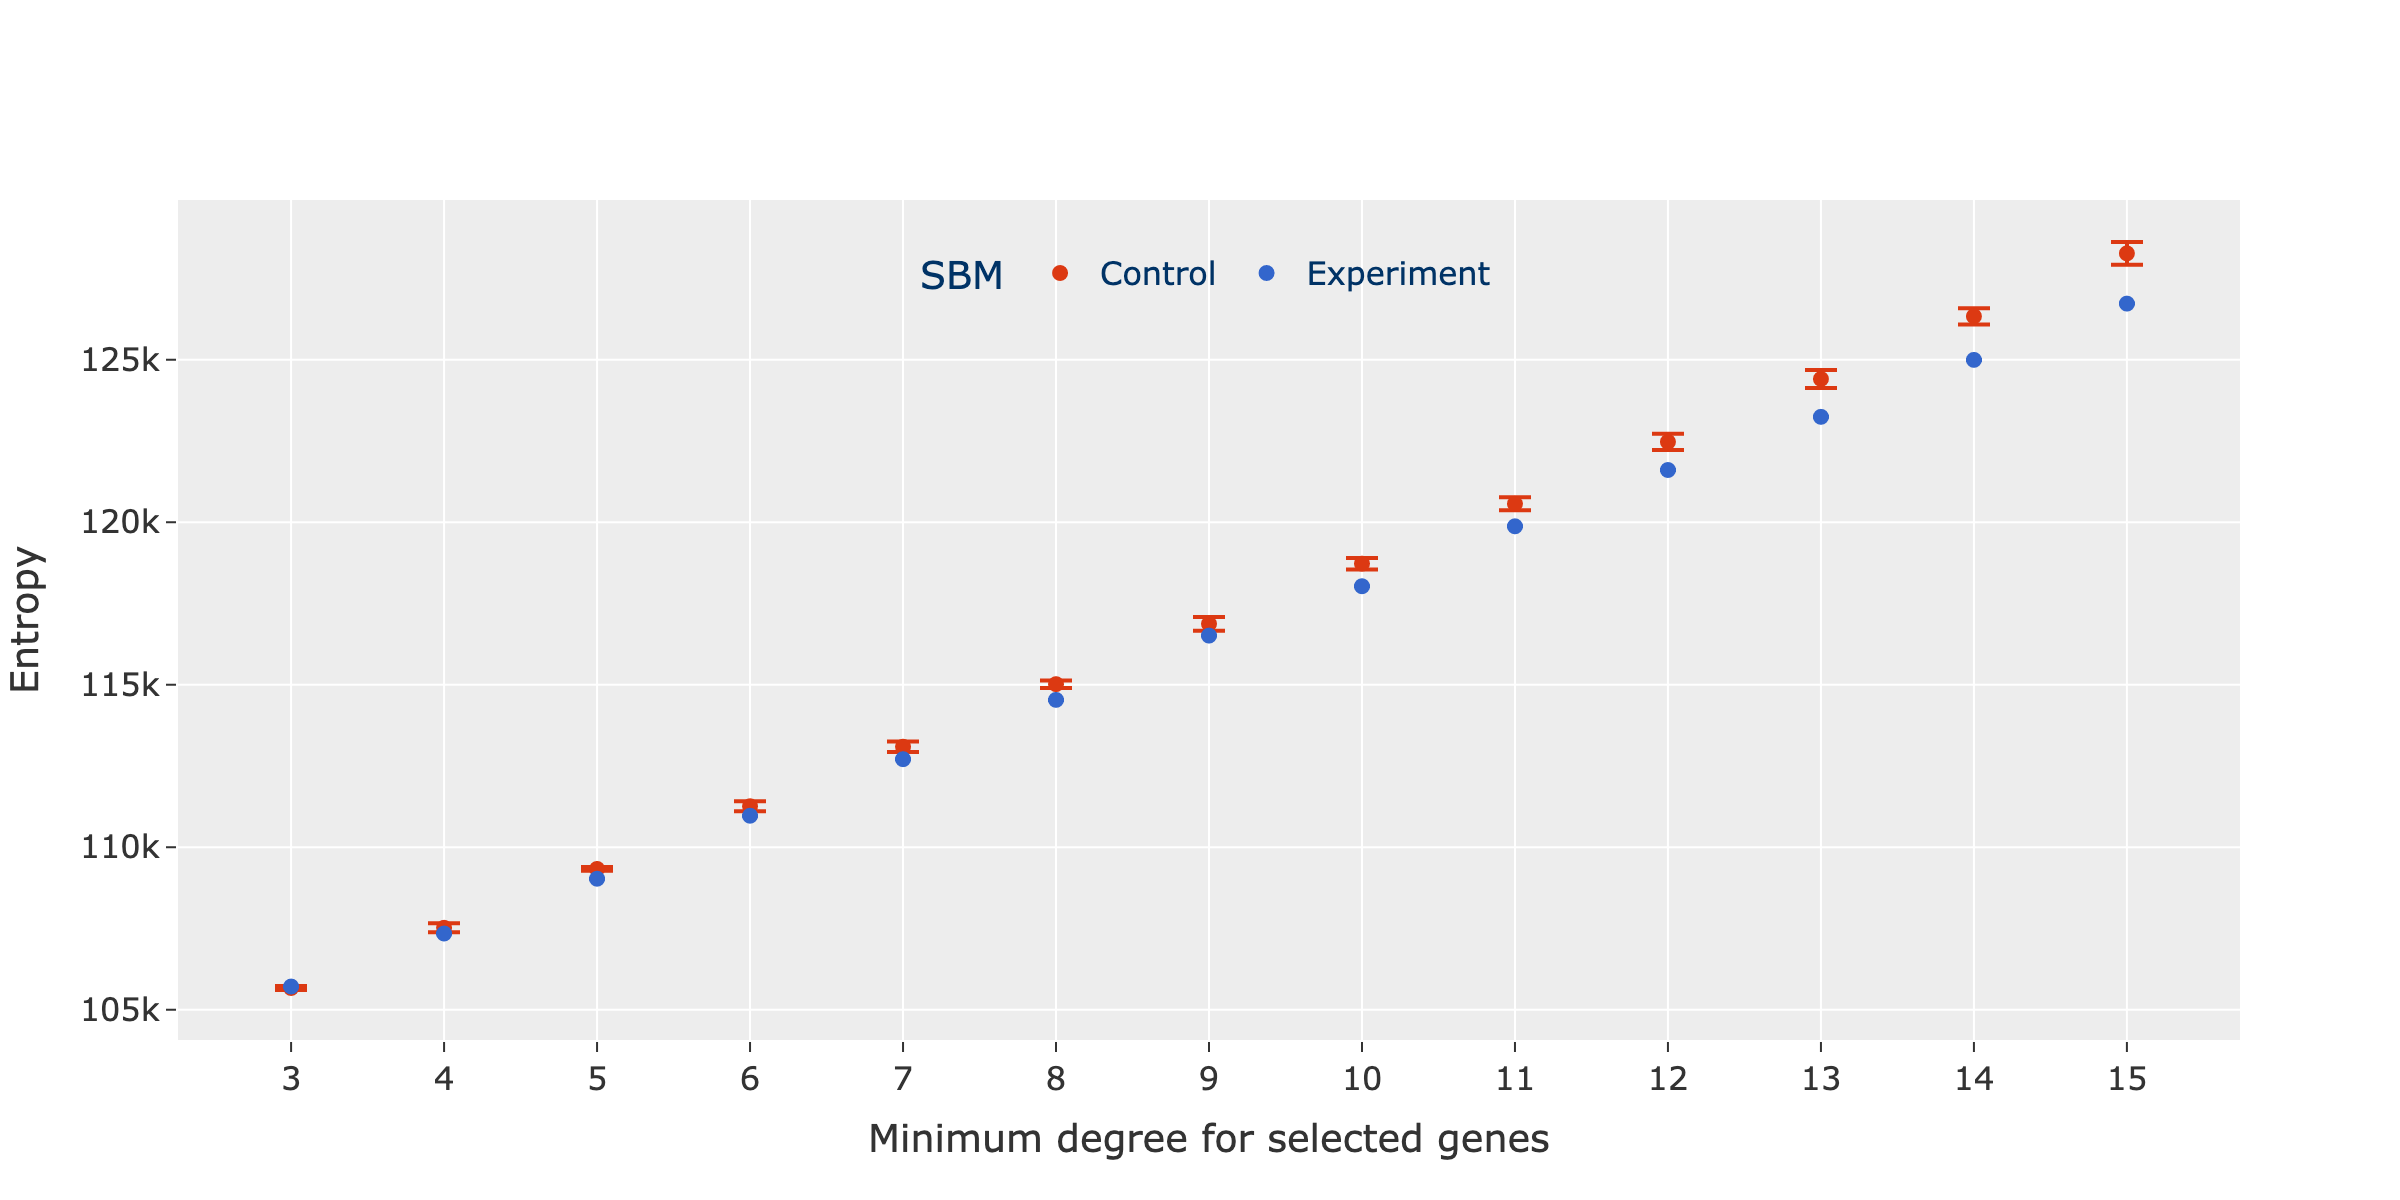
\includegraphics[width=\textwidth]{Sections/Network_I/Resources/selective_pruning/sbm_ent_sel_prun.png}
        \caption{SBM}
        \label{fig:N_I:sbm_com_det_met}
    \end{subfigure}\hspace{\fill} 
    \begin{subfigure}[!t]{0.5\textwidth}
        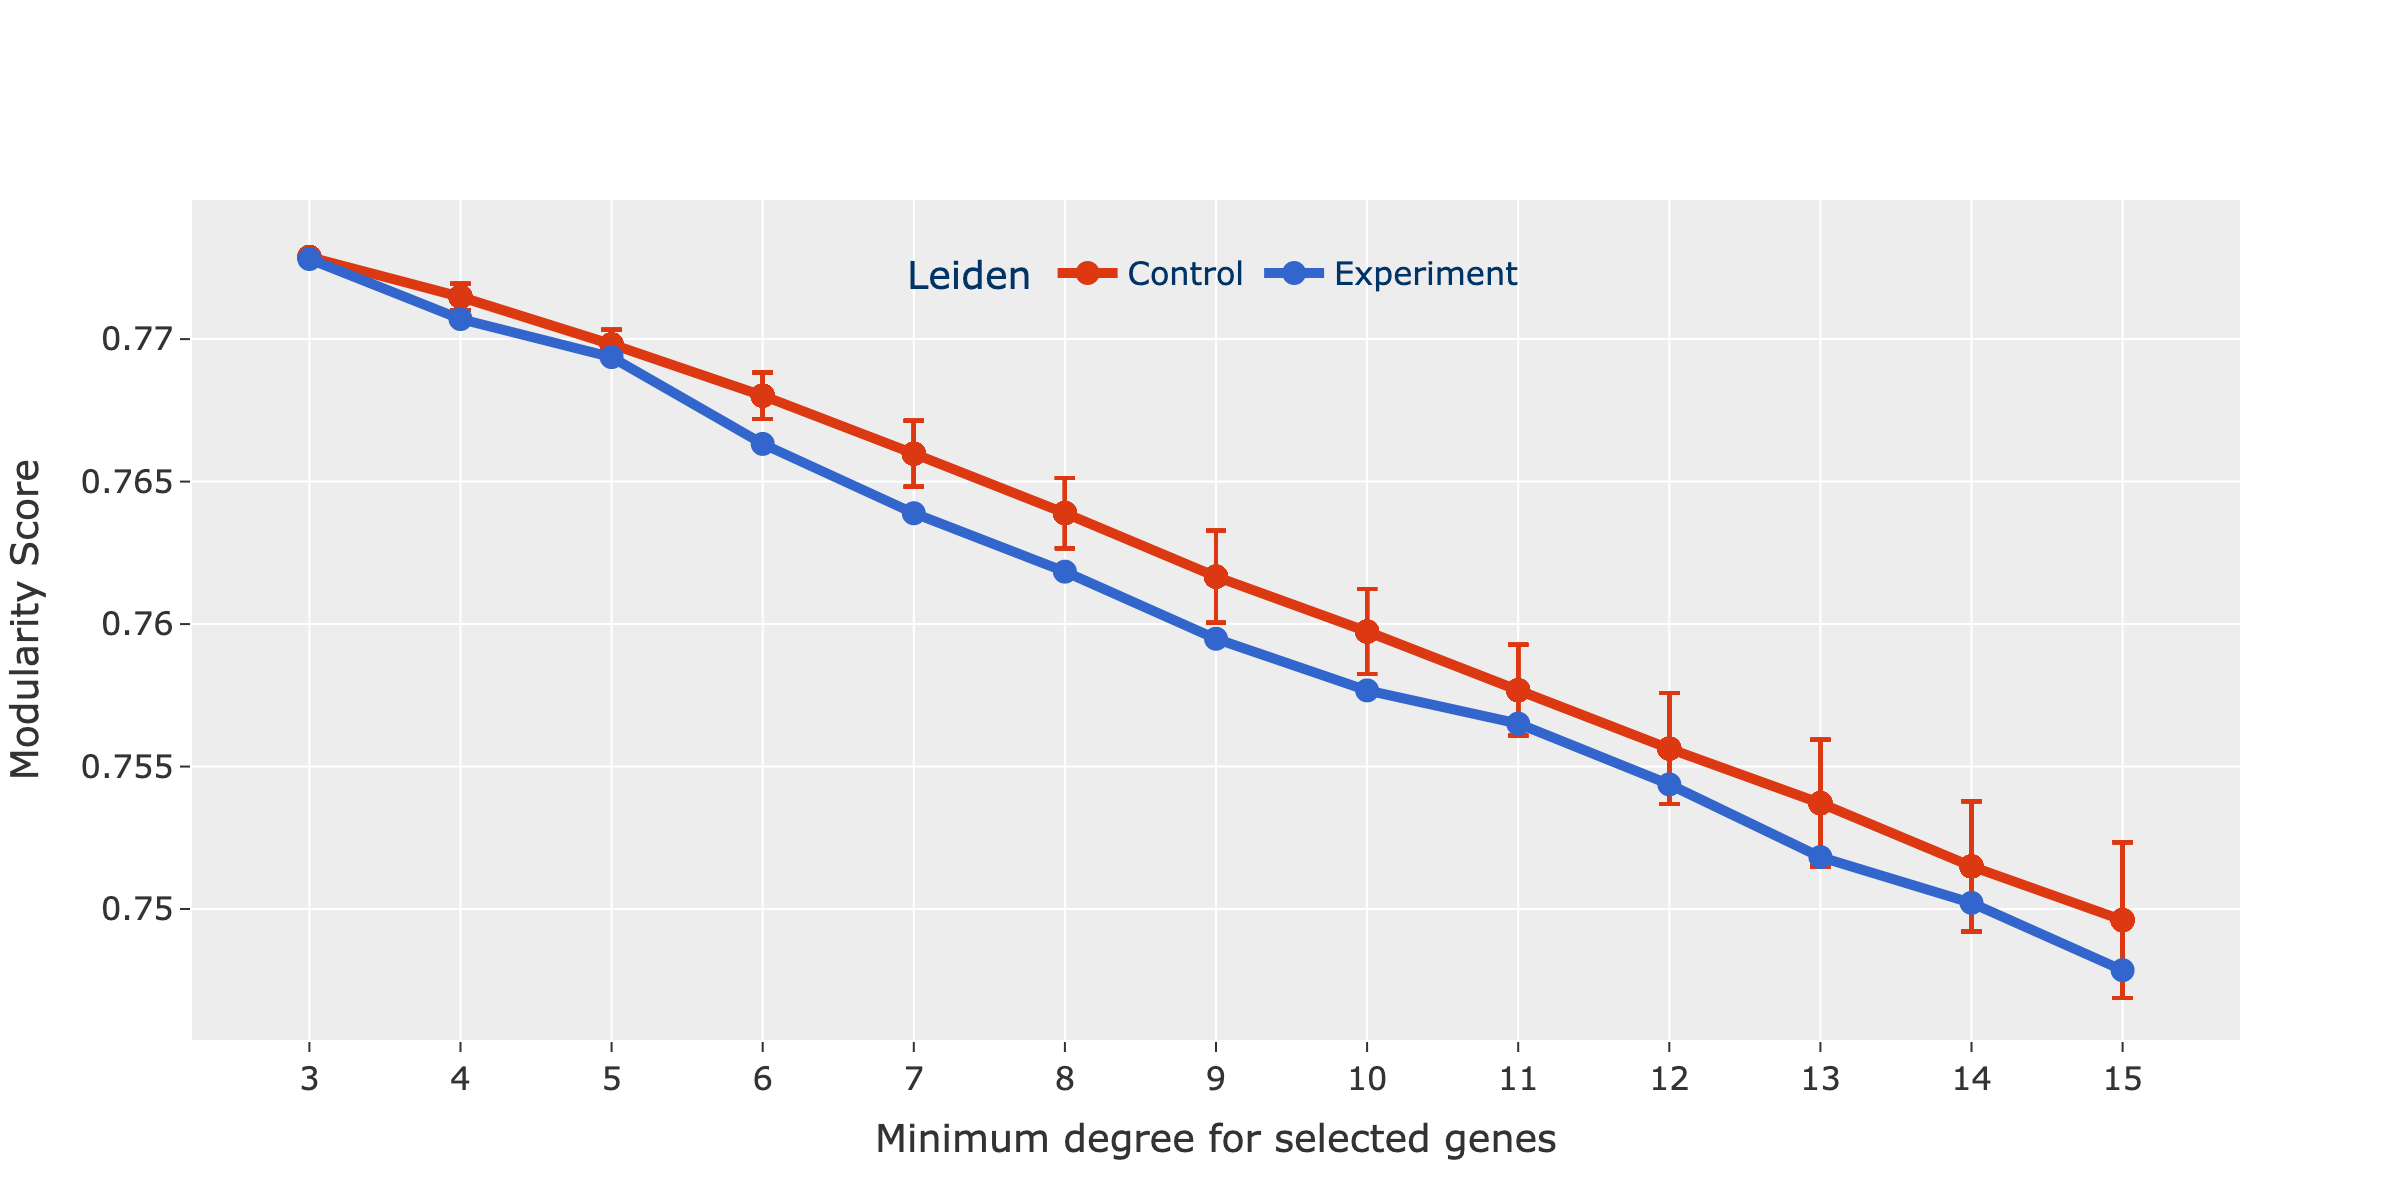
\includegraphics[width=\linewidth]{Sections/Network_I/Resources/selective_pruning/leid_mod_sel_prun.png}
        \caption{Leiden}
        \label{fig:N_I:leid_com_det_met}
    \end{subfigure}
    \caption{Metrics comparison between Minimum Description Length (MDL) - entropy- in SBM (lower the better) and Modularity Maximisation in Leiden (higher the better). As the minimum degree for the increases both community detection suffer a decrease in the performance. he error bars in the control is given by the standard deviations.}
    \label{fig:N_I:com_det_met}
\end{figure}

% Comment com_size figure
In \cref{fig:N_I:comp_size_com_det} it is presented the effect to the of increasing the minimum degree to the community sizes to the two community detection algorithms. The blue traces represent the Experiments performed while the red controls. The immediate difference between Leiden and SBM is that the former finds consistently considerably more communities than the latter. It can be noticed that SBM has an upward trend proportional with the minimum degree of the nodes, this highlighted by the control experiments. In \cref{fig:N_I:comp_size_com_det}, Leiden appears to find the same number of clusters, but in the \cref{fig:ap:leid_com_size} from Appendix, where the Leiden traces are plot separately, it can be notice that Leiden tends to finds less communities as the minimum degree it is increased. 

\begin{figure}[!htb]   
\centering
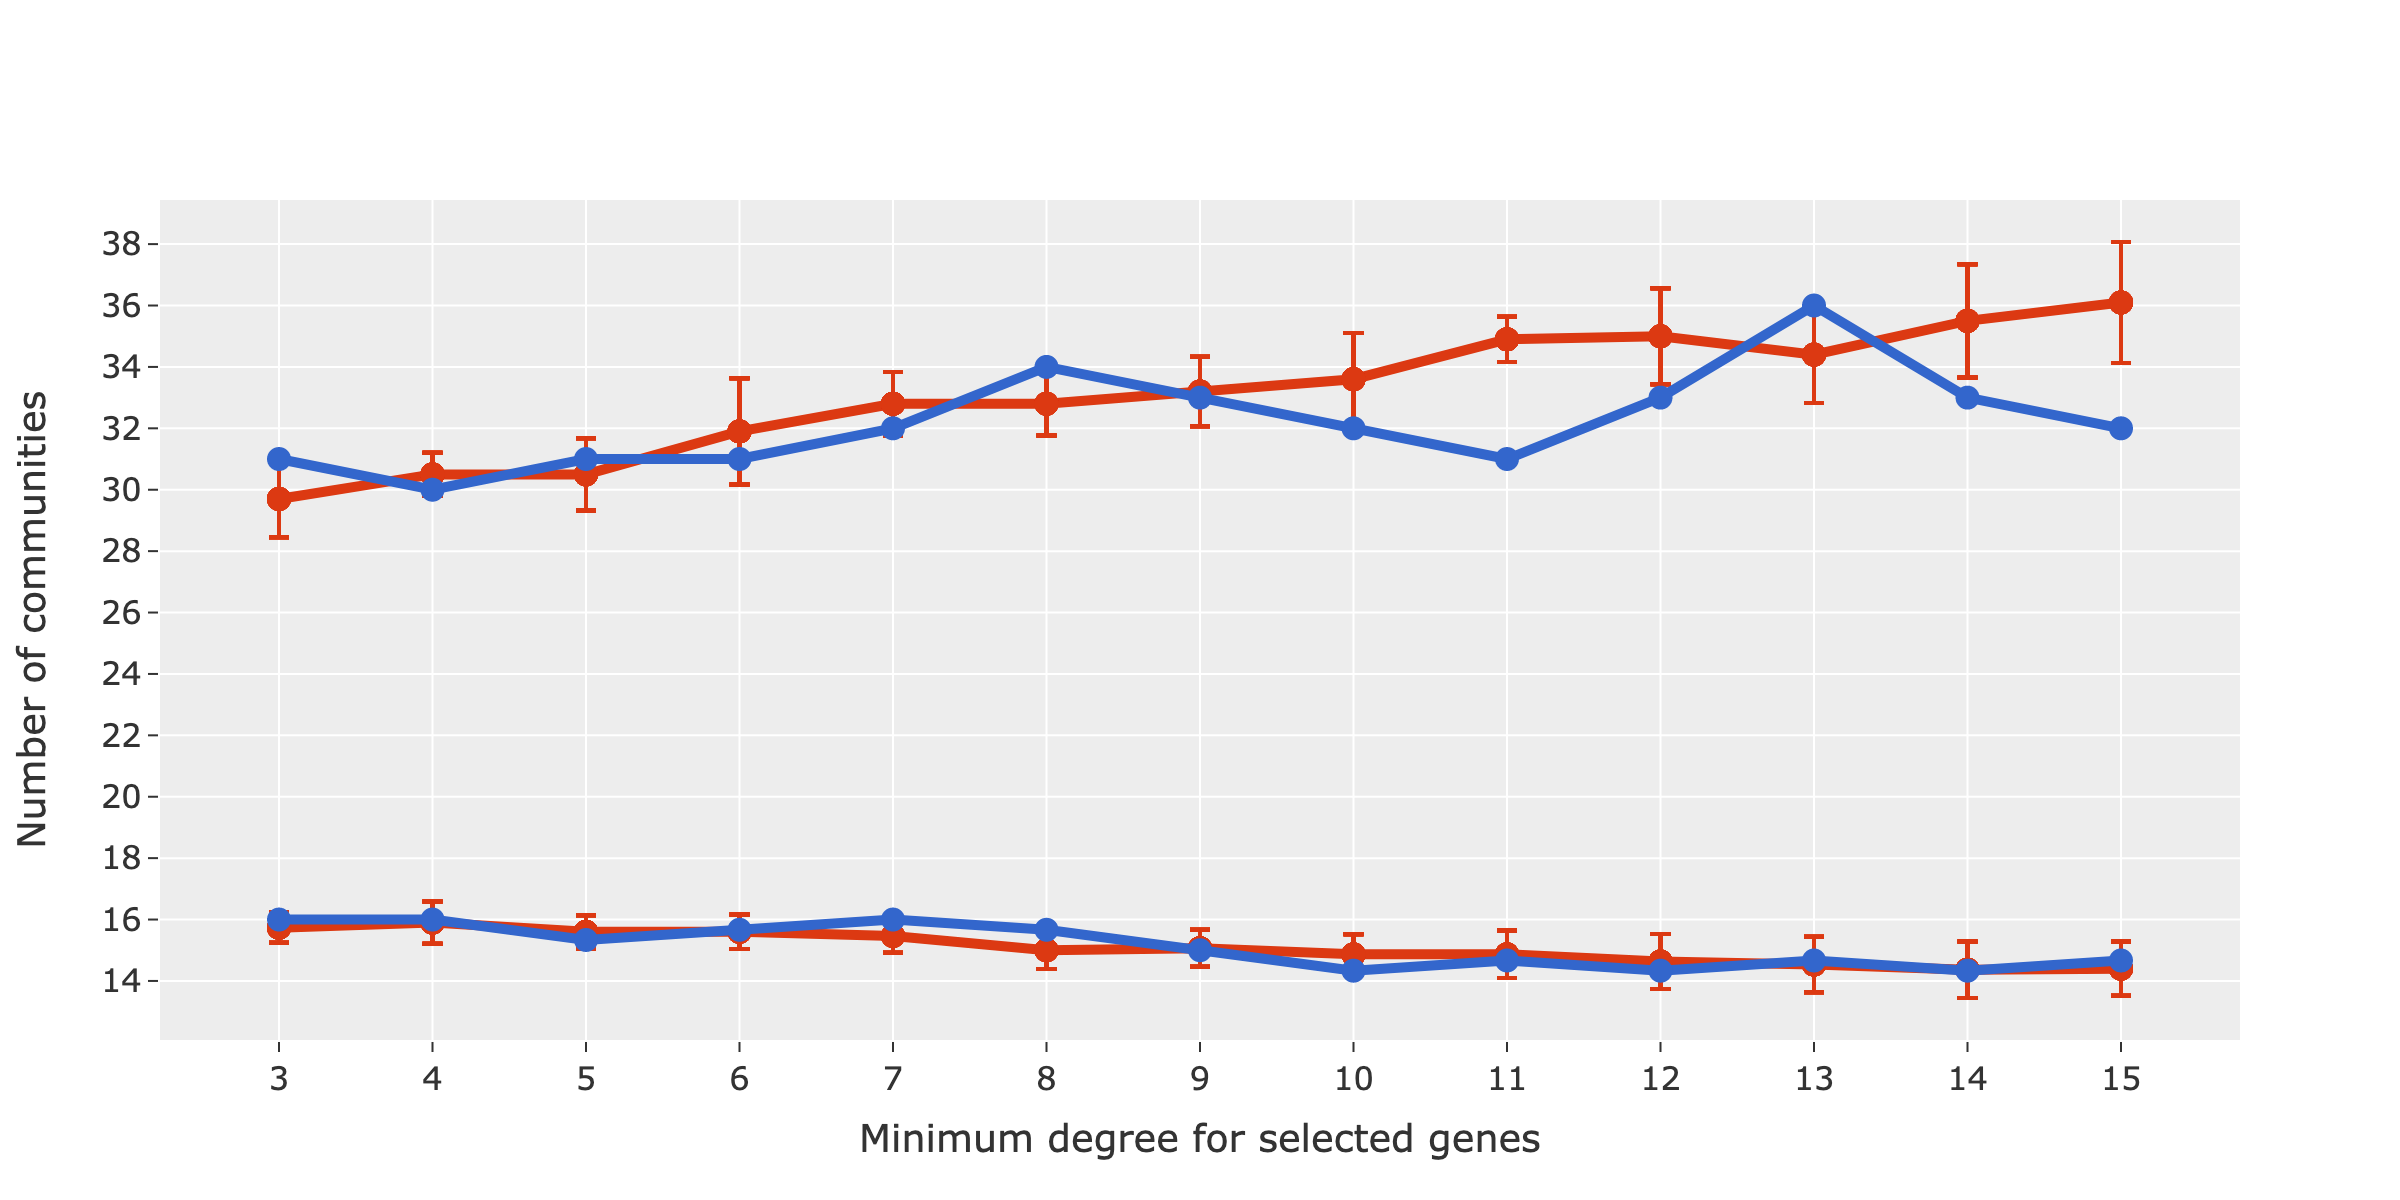
\includegraphics[width=1.0\textwidth,height=1.0\textheight,keepaspectratio]{Sections/Network_I/Resources/selective_pruning/sbm_Leiden_combNum.png}
  \caption{Community size for Leiden and Stochastic Block Model. Blue lines are represented by the experiments run with biological TFs while the red ones are the controls, with non-TF genes. The error bars in the control is given by the standard deviations.}
\label{fig:N_I:comp_size_com_det}
\end{figure}

% Variance and that SBM is probabilistic
Growing the number of nodes also increases the variance in the number of communities found by the two methods. This can be more clearly seen in \cref{fig:ap:com_size_comp}, which also shows that SBM has a higher variance compared to Leiden. However, due to the probabilistic nature of SBM and the fact that each set of communities is found after 700 iterations, it is possible to observe module oscillations as well as changes in gene memberships. This helps identify genes that change community membership as well as the 'stable' genes.

% Summary
In summary, by increasing the minimum degree, both algorithms perform worse regardless of whether the prioritised genes are selected at random or have biological significance (i.e., TFs). SBM finds more communities compared to Leiden but has a higher variance. Given the probabilistic nature of SBM, additional useful information can be extracted from the network like gene membership. For these reasons, and because SBM does not find patterns in noise, the stochastic model is the preferred method in this project.


% Analysing the TFs
\subsection{Emerging Transcription Factors} \label{s:N_I:sel_tfs}

% Introduce the motivation of using TFs
After comparing the two community detection algorithm and deciding on the SBM, it is worth diving in the analysis of the network output. The previous sub-section showed that by prioritising a certain subset of genes, to have a higher minimum degree, has some effects on the network. However, in the network pipeline, not all the genes employed to generate the graph are used for the cancer stratification, but the top 100 selected by ModCon (see \cref{fig:N_I:network_pipeline}). The ModCon score is a score which takes in account a node's number of edges and their weights, thus higher connected genes are selected.

% Presentin the Graph of sel TF-s. 
% -- all TF are included when minimum degree is set to 15 and there is no added benefit when TF = 6
\Cref{fig:N_I:sel_tfs} show the percentages of the TF genes (325 in total) that are selected by the ModCon score to stratify the disease. SBM community detection was used with both selected genes that are TF and non-TF 325 genes as control, the latter was run 10 times. It can be seen a clear difference between the Experiment and the Control traces, where the genes in the Experiment, with a real biological value, gradually increase with the minimum degree values. All the TF genes are included when the minimum degree of a TF reaches to 15 and the biggest percentage included after TF passes minimum degree of 6. Therefore, this value was chosen for selective edge pruning.


\begin{figure}[!ht]   
\centering
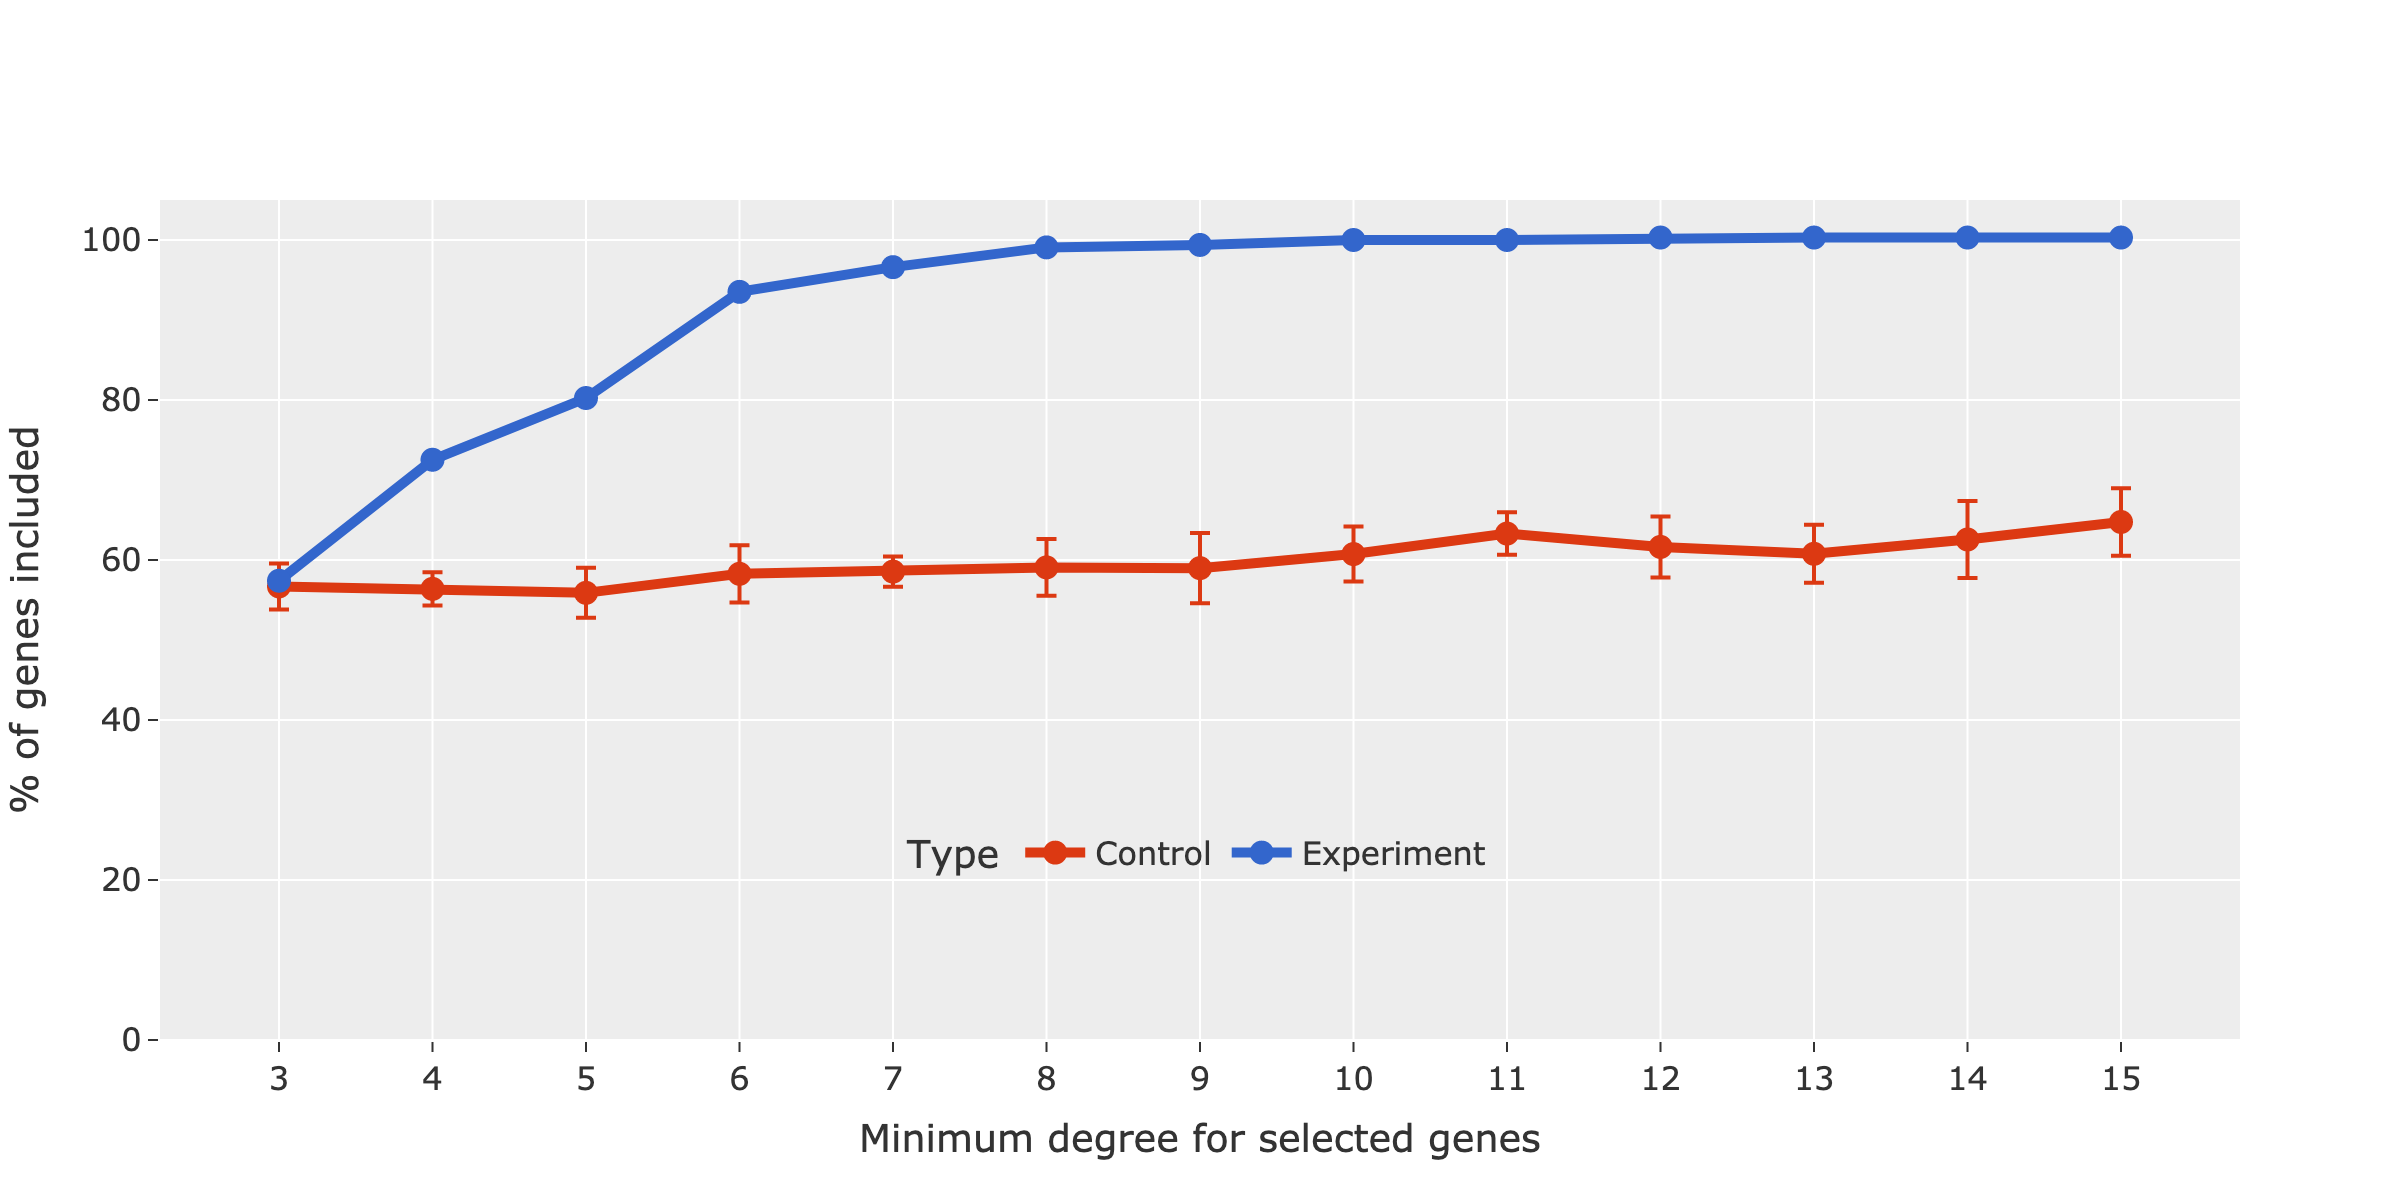
\includegraphics[width=1.0\textwidth,height=1.0\textheight,keepaspectratio]{Sections/Network_I/Resources/selective_pruning/ctrls_min_dig_mev.png}
  \caption{The percentages of the Transcription Factors selected by ModCon as the minimum degree increases.}
\label{fig:N_I:sel_tfs}
\end{figure}

% Biological relevance
% -- Because 50% of the TF naturally emerges and used for subtyping
On contrast to the Experiment trace, the Control appears to have a constant number of biological TFs selected by ModCon, of $\sim60\%$. This means that there are a subset of the TFs which are consistently picked by ModCon (i.e. with a high connectivity) despite other than 325 TFs were allowed a high number of connections. 

% Highlighting the importance
To explain this behaviour, it is worth re-surfacing the selective edge pruning process. For each gene in the correlation matrix only the 3 highest correlated genes are kept for standard genes or 6 for the selected genes to prioritise. Thus, a gene can have a starting degree either of 3 or 6. For a node $A$ to have higher a degree, it needs that other genes to have node A in their top correlation. For example, if node $A$ is a non-TF gene and it has a degree value of 10, it means that 7 other genes have node $A$ in their top correlations

% Biological significance
Taking in account the selective edge pruning and that $\sim60\%$ of the 325 TF genes are selected by ModCon, when the TF are \textbf{explicitly} not prioritised, it is remarkable to have a subset of genes that emerged as being highly connected. To further refine the list, the intersection of genes across the controls is taken and this leads to a list of 98 TF, that are constantly highly connected across the controls. The next section analysis this list of TF in depth. 

\begin{figure}[!ht]   
\centering
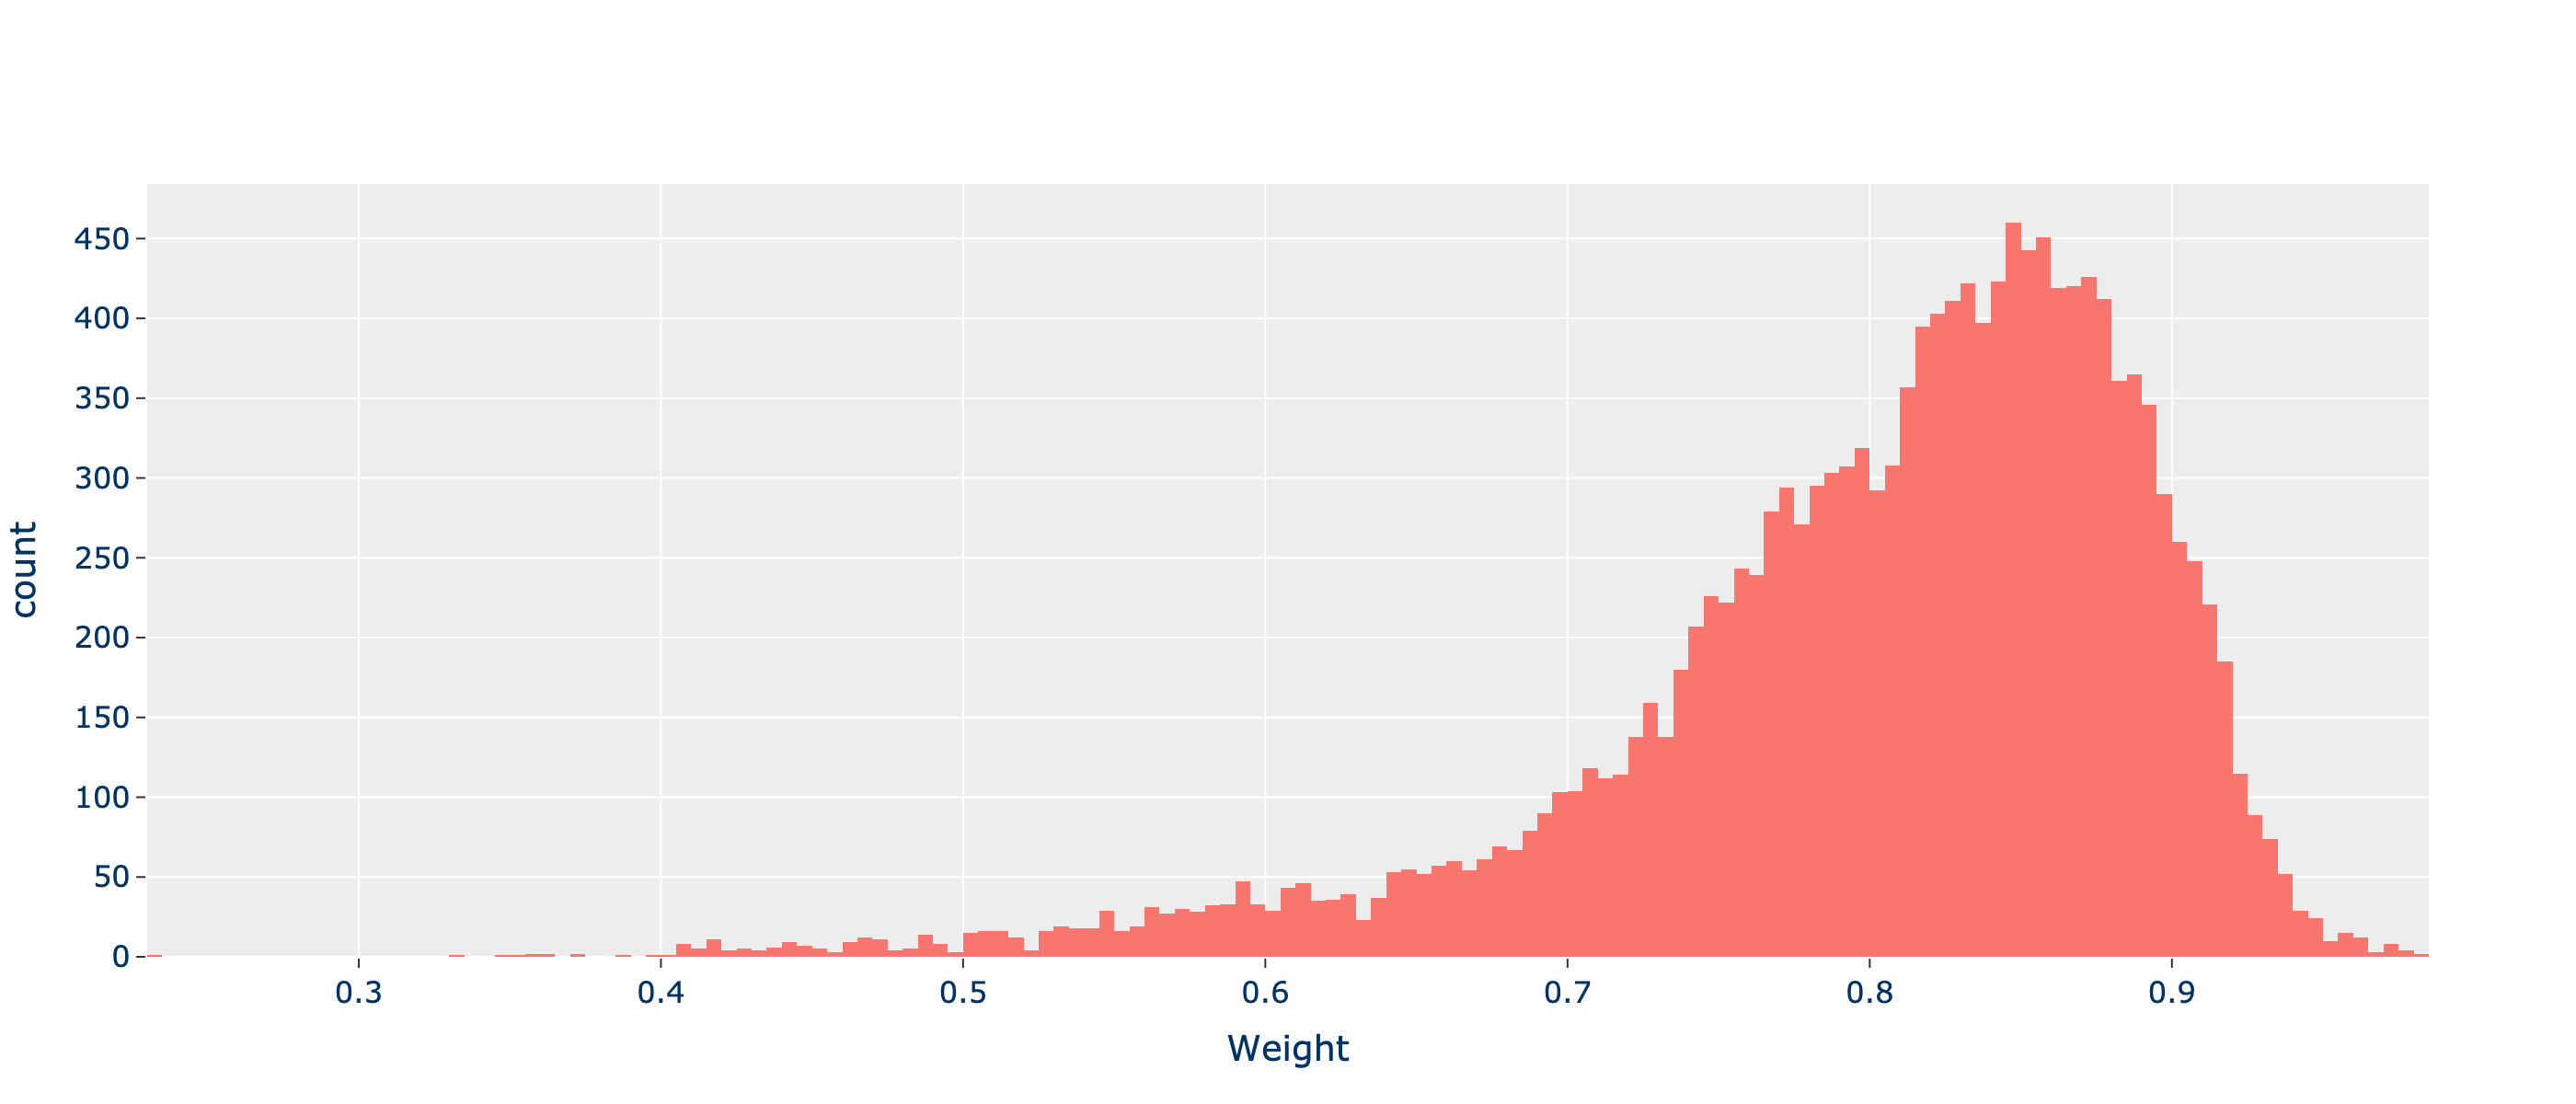
\includegraphics[width=1.0\textwidth,height=1.0\textheight,keepaspectratio]{Sections/Network_I/Resources/selective_pruning/weight_distrib.png}
  \caption{The weight distribution of the edges weights in a standard network (no weight modifier), with 3 edges for non-TF and 6 for TF genes.}
\label{fig:N_I:weight_distrib}
\end{figure}

% Shows that the selective edge pruning only selects the highly correlated genes
In the selective edge pruning strategy introduced by \citet{Care2019-ij} there is no threshold to ensure that the low correlated pair of genes are not cluttering the network and that the most co-expressed pairs are kept. To test this the weight distribution is plot in \cref{fig:N_I:weight_distrib} for a standard network with no weight modifiers, with a minimum 3 edges per standard gene and 6 per TF. It can be seen that the distribution is skewed right, ensuring that most of the genes are highly correlated.

% Clustering
\subsubsection*{Clustering}


% Talk about the clustering
Hierarchical clustering was applied to the tumour expression of the 98 TFs after 11 samples previously identified as outliers were removed\footnote{In this context, outliers are samples that cluster in 1-3 groups, making it hard to interpret the dendrogram from the hierarchical clustering}, leaving 392 samples for clustering. The tumour\footnote{TCGA's MIBC cohort} data was log2(TPM+1) transformed, normalised by the quantiles, and then agglomerative clustering with average linkage was applied on the 1-Pearson correlation distance\footnote{In this case, for both clustering and visualisation, Morpheus from the Broad Institute was used \cite{Broad-InstituteUnknown-kn}}. This method was preferred over those developed in the previous chapter because the number of genes was small and the heatmap from Morpheus is a useful tool for showing the gene expression specific to a group. The heatmap and the output are shown in \cref{fig:ap:morph_sel_tfs} in the Appendix.

% describe morpheus
A dendrogram cut of 15 was chosen as it split both the Luminal and Basal Groups and there are relatively small groups. From the heatmap \cref{fig:ap:morph_sel_tfs} it can be noticed that there is a large group of Luminal samples and a smaller one. The Basal group is split into three subgroups, a large one, a medium size which groups most of the Mes-like tumours from Lund classifier and a smaller ones which has a lower Infiltration/Stromal/Estimate scores compared to the other 2 Basal groups. Apart from these 2 groups, there are outliers samples that are grouped in 1 or 2 clusters, suggesting that they have particular molecular profiles.

\begin{figure}[!t]
\centering
    \captionsetup[subfigure]{justification=Centering}
% Sankey - consensus and K-means comparison
\begin{subfigure}[!t]{0.49\textwidth}
    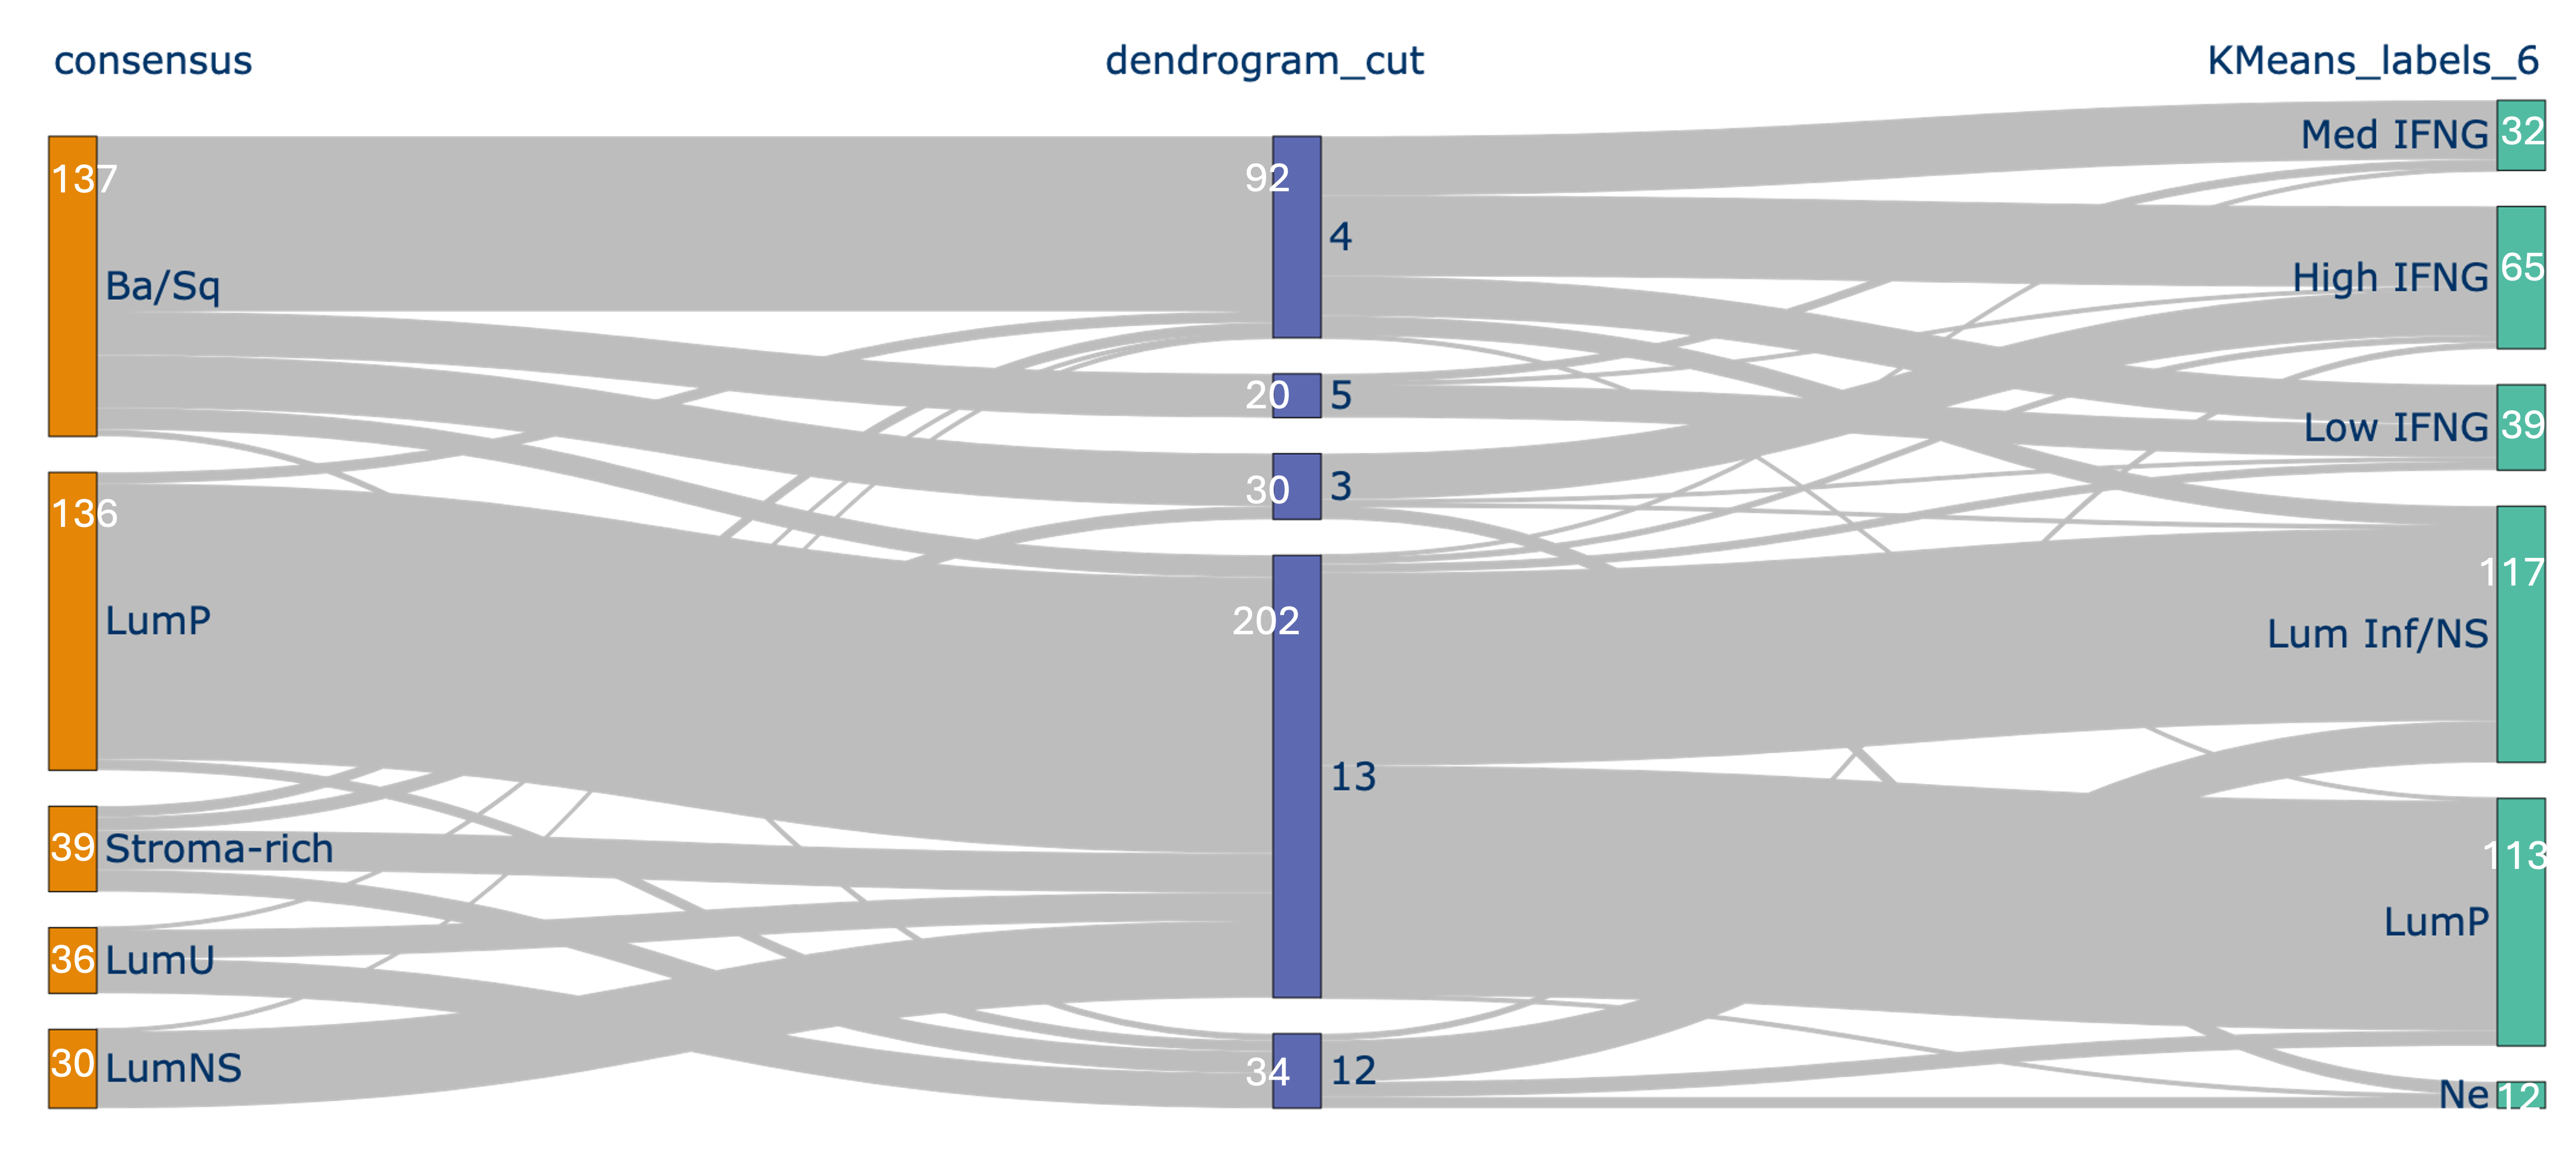
\includegraphics[width=1.0\textwidth,height=1.0\textheight,keepaspectratio]{Sections/Network_I/Resources/selective_pruning/sankey_sel_tfs_VU_CS.png}
    
    \caption{Sankey plot comparison between the hierarchical clustering from \cref{fig:ap:morph_sel_tfs}, consensus \cite{Kamoun2020-tj} and clustering performed in the earlier chapter \cref{s:lit:clustering}.}
    
    \label{fig:N_I:sankey_sel_tfs_vuCs}
\end{subfigure}
\hfil %necessary to have the two subpltos near each other
% Sankey - TCGA and Lun comparison  
\begin{subfigure}[!t]{0.49\textwidth}
    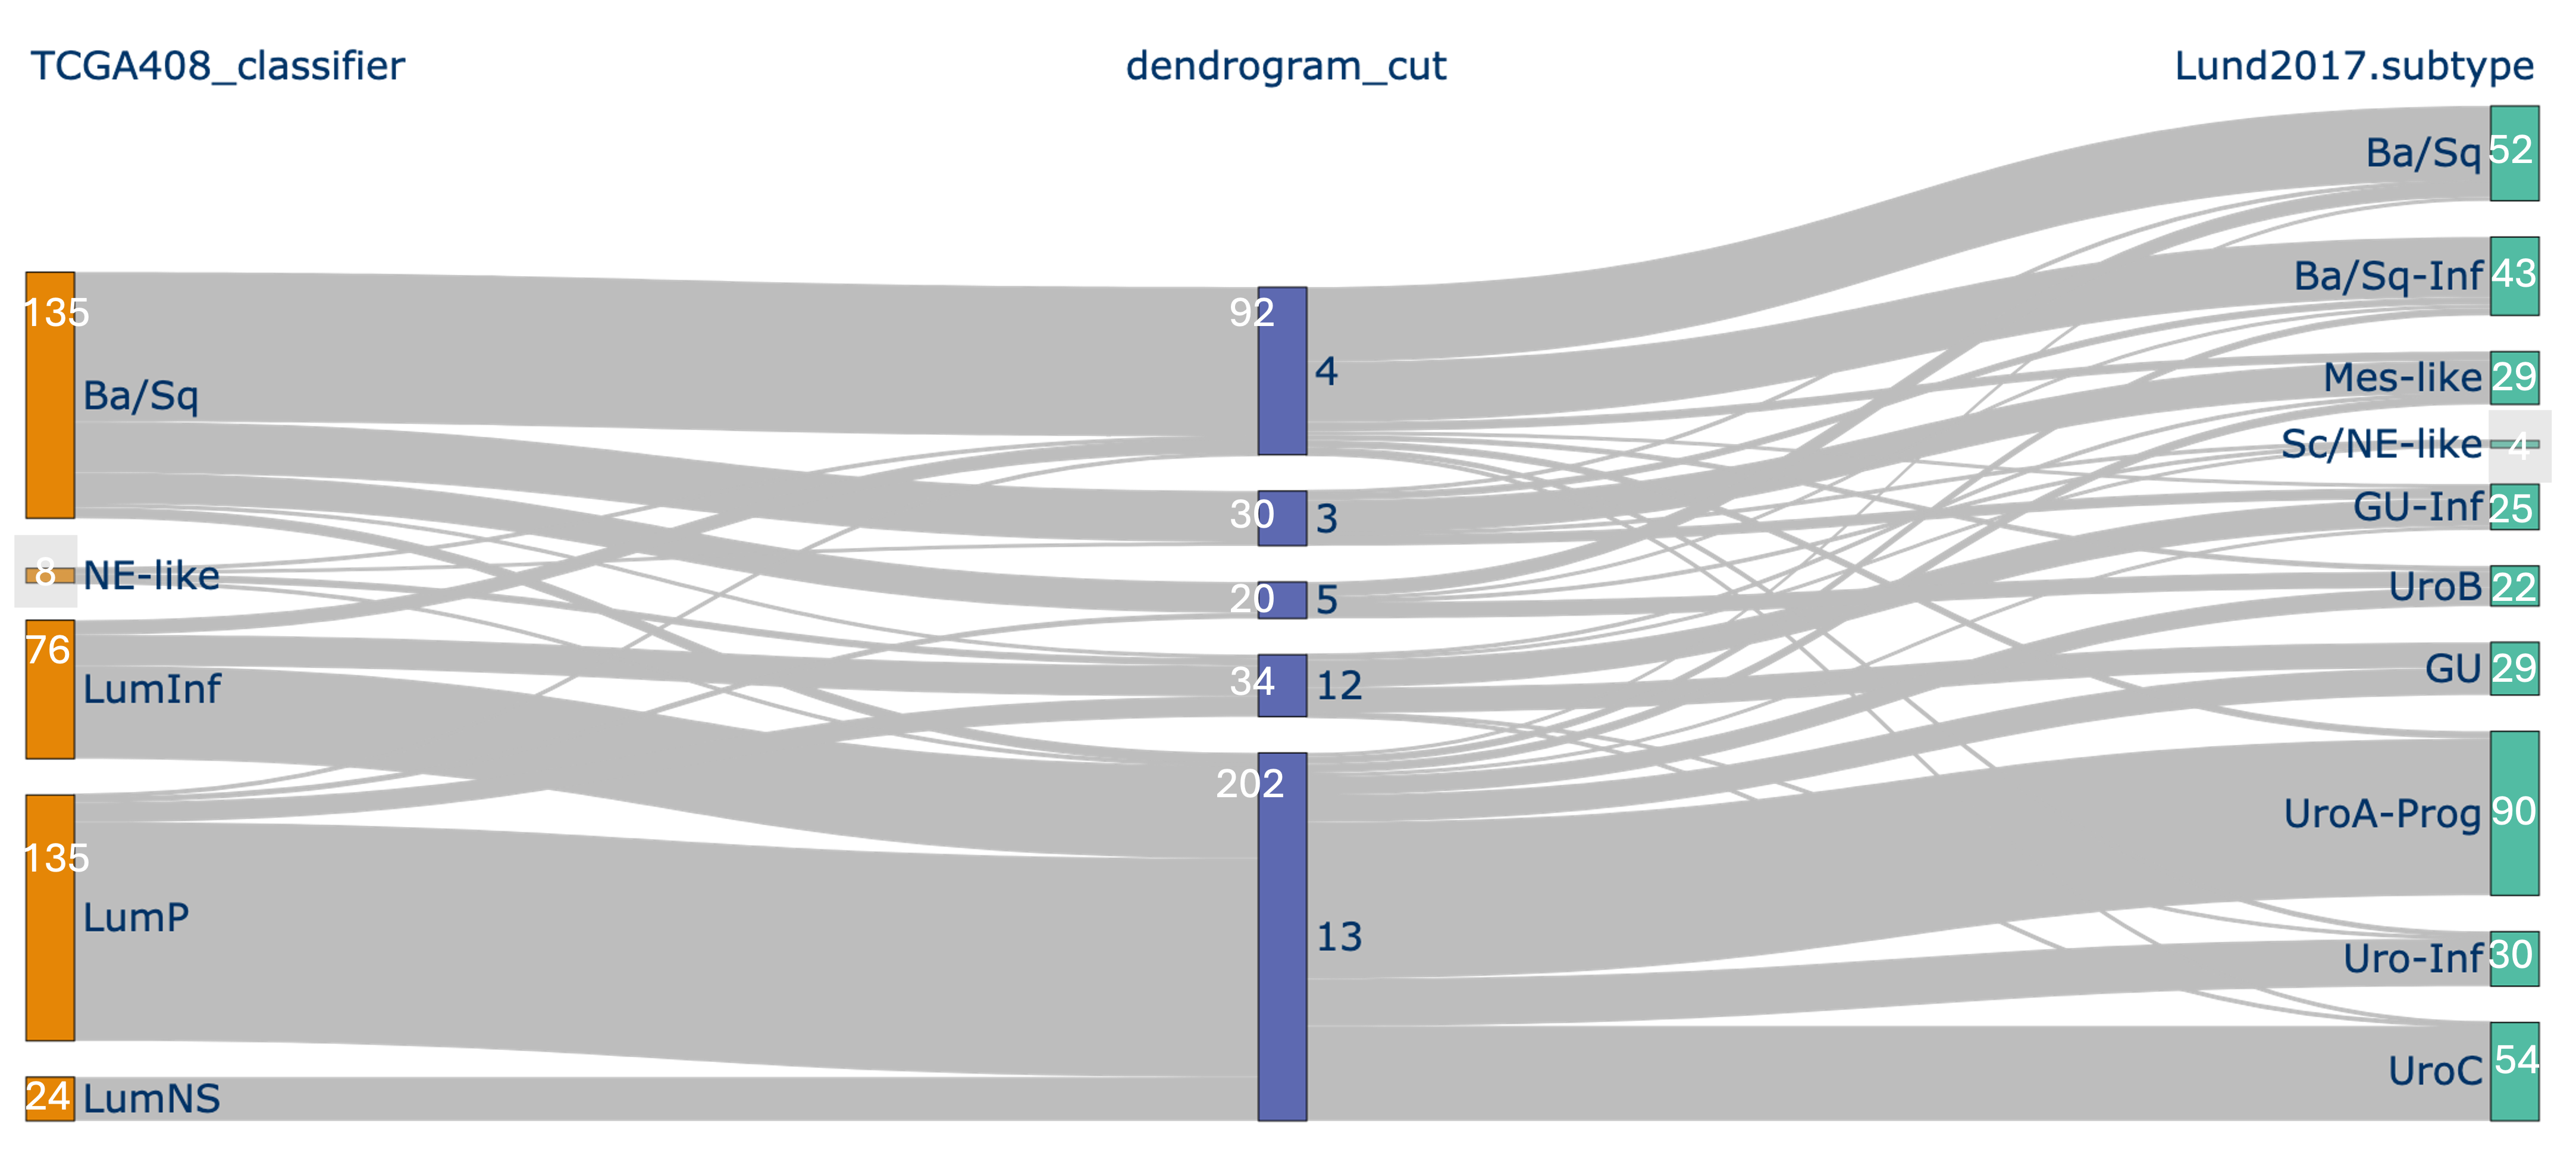
\includegraphics[width=1.0\textwidth,height=1.0\textheight,keepaspectratio]{Sections/Network_I/Resources/selective_pruning/sankey_sel_tfs.png}
    
    \caption{Sankey plot comparison between the hierarchical clustering from \cref{fig:ap:morph_sel_tfs}, TCGA \cite{Robertson2017-mg} and Lund \cite{Marzouka2018-ge}.}
    
    \label{fig:N_I:sankey_sel_tfs}
\end{subfigure}
% Survival
\centering
\begin{subfigure}[!t]{0.7\textwidth}
    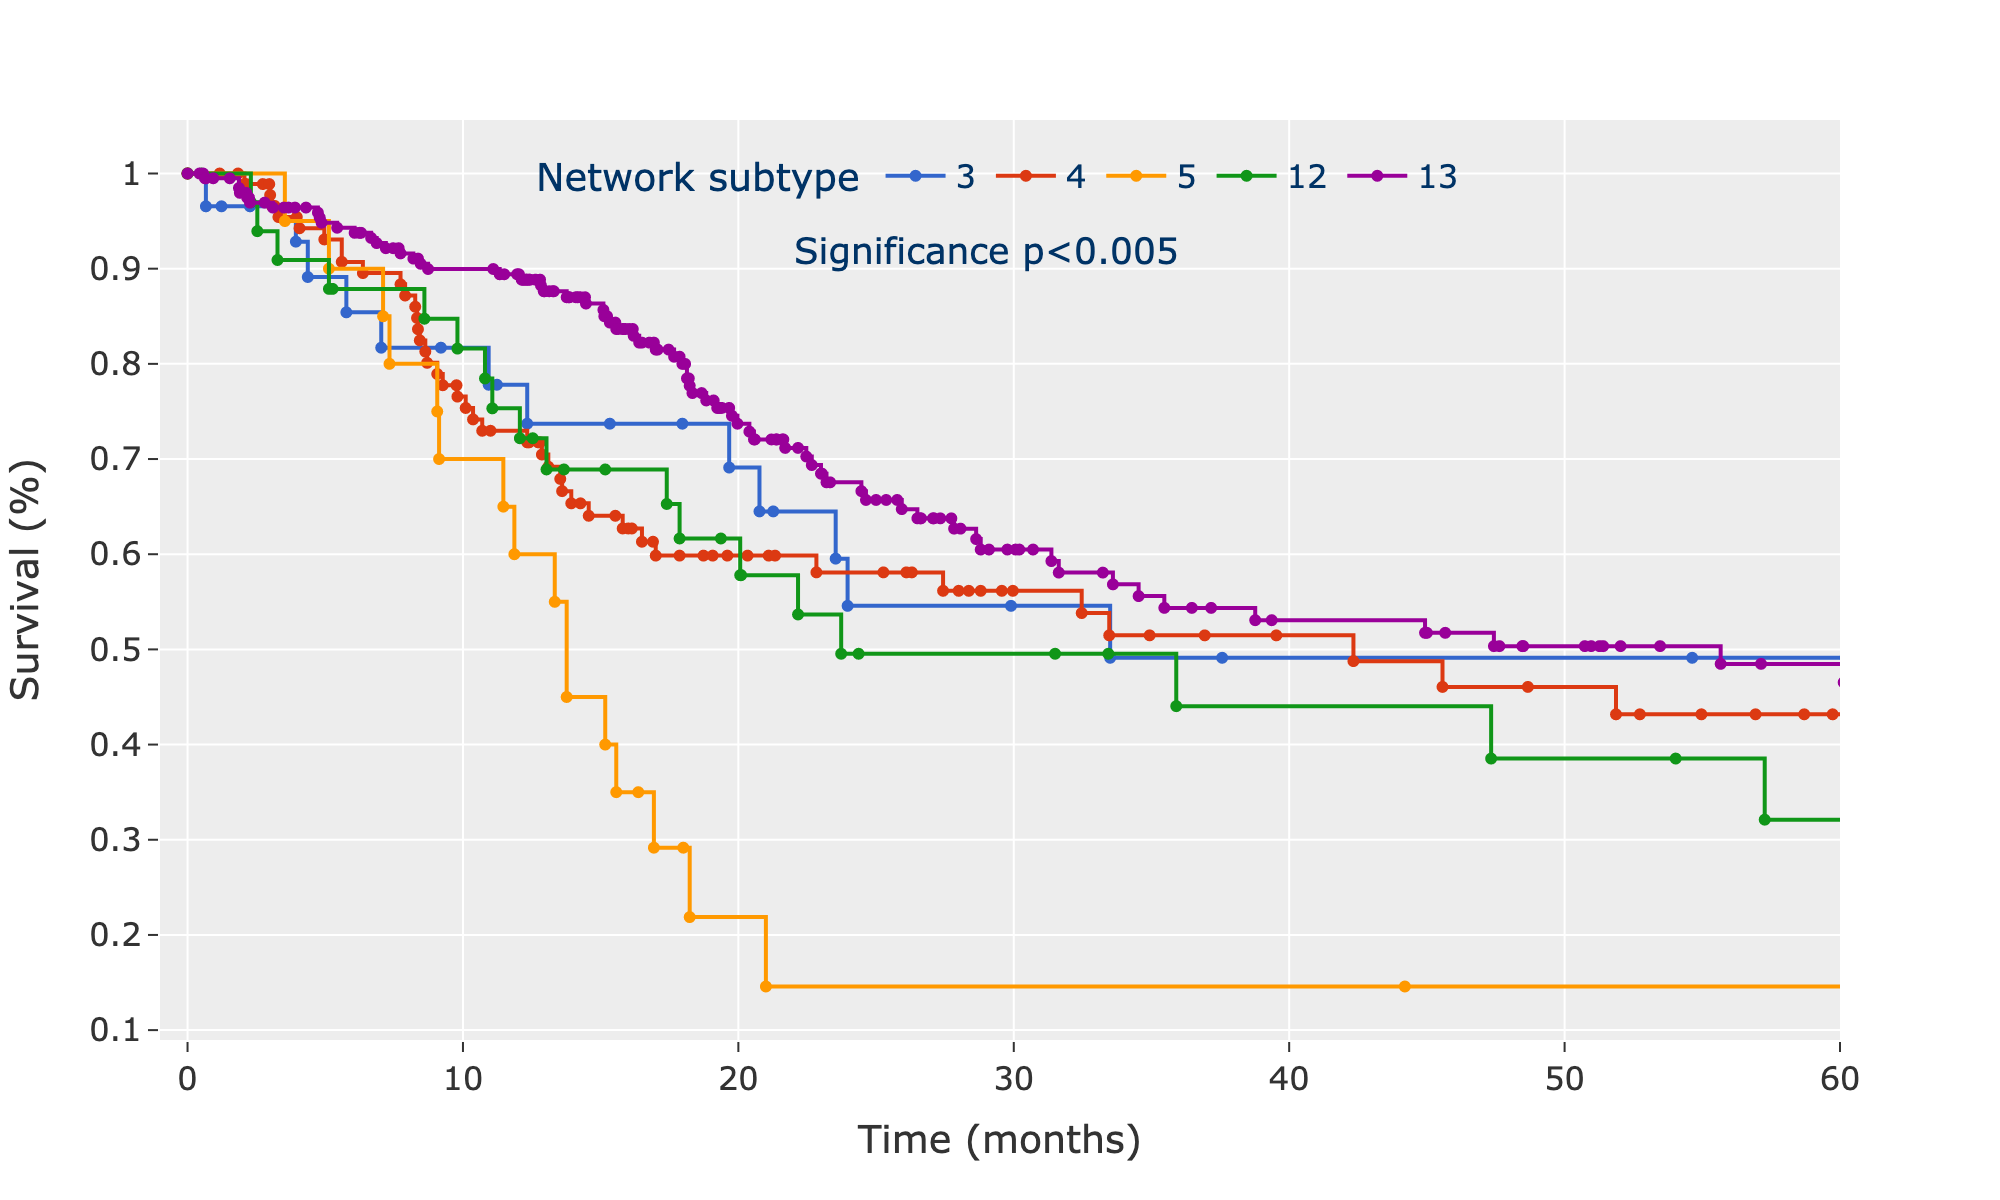
\includegraphics[width=1.0\textwidth,height=1.0\textheight,keepaspectratio]
    {Sections/Network_I/Resources/selective_pruning/survival_sel_tfs_cs.png}
    \caption{Kaplan-Meier survival analysis of the groups found with the 98 TFs. }
    \label{fig:N_I:sel_tfs_survival}
\end{subfigure} 

    \caption{Cluster analysis of the subgroups derived using the found 98 TFs. The top row represent the subtype comparison with previous works while the bottom figure is Kaplan-Meier survival plot. The white text on the Sankey plots represents the size of the groups.}
    \label{fig:N_I:sel_tfs_cs_analysis}
\end{figure}
 
% Describe Sankey
The groups smaller than 1\% of the cohort size (equivalent to 4 samples) are removed, resulting in a dataset of 378 samples grouped into 5 major groups. These subtypes are compared in \cref{fig:N_I:sankey_sel_tfs_vuCs,fig:N_I:sankey_sel_tfs} with previous work from Lund \citet{Marzouka2018-ge}, TCGA \citet{Robertson2017-mg}, consensus \citet{Kamoun2020-tj}, and the subtyping clusters found in the previous chapter \ref{}. 

% Luminal groups
In the comparison (\cref{fig:N_I:sankey_sel_tfs_vuCs}) with the consensus and the clusters from the previous section \ref{}, it can be noticed that there is a large luminal group (13) consisting of 202 samples. The group contains most, if not all, of the samples from LumP, Stroma-rich, LumU, and LumNS (consensus) and the LumInf/NS and LumP (KMeans\_6). This is also the case in \cref{fig:N_I:sankey_sel_tfs}, where group 13 contains the LumInf, LumP, LumNS (TCGA) and the UroA-Prog, Uro-Inf, and UroC from Lund. The smaller luminal group (12) consists mostly of the samples from LumU, Stroma-rich from TCGA (\cref{fig:N_I:sankey_sel_tfs_vuCs}) or the consensus LumInf/LumP (TCGA) or the Genomically Unstable (GU) and GU-infiltrated from Lund. 

% Basal subgroups
The larger group, consisting of 92 samples, is formed of a mix of samples from Medium, High, and Low IFNG (KMeans\_6) and Ba/Sq samples from the consensus. The medium-sized group is a combination of the High IFNG and Ne subgroups from KMeans\_6, while the smaller-sized group is formed of Low IFNG and Med IFNG. Switching to the comparison with TCGA/Lund (\cref{fig:N_I:sankey_sel_tfs}), it can be noticed that the large basal group (4) contains most of the Ba/Sq (TCGA) or Ba/Sq and Ba/Sq-infiltrated (Lund) samples. The medium-sized (3) basal cluster contains most of the Mes-like samples (Lund), while the smaller group (5) consists of UroB and Ba/Sq (Lund) samples. Thus, the MIBC stratification on the 98 TFs exhibits one major (large) basal group (4), a medium-sized (3) group which contains the Mes-like samples from the Lund classifier or the samples from High IFNG, and the small basal group (5) consisting of low IFNG samples or a combination of the UroB and Ba/Sq samples. It is worth mentioning that the UroB (Lund) and Low IFNG have a low survival prognosis, while High IFNG has a good prognosis.

% Summary of the comparison
The comparison with the other stratification methods shows that clustering the expression of 98 TFs is capable of finding three basal subtypes, two smaller even than the ones found in the previous chapter \ref{}. However, the 98 TFs fail to discriminate the luminal subgroups.

% Survival analysis
\subsubsection*{Survival Analysis}

Survival analysis was conducted on the five groups derived from the 98 transcription factors as shown in \cref{fig:N_I:sel_tfs_survival}. Group 5, identified as the smallest basal group, exhibits the poorest survival prognosis by a significant margin. Notably, the poorest survival in both the TCGA and consensus classification is observed in the Neuroendocrine-like groups, which are not included in Group 5; this is illustrated in the Sankey plot in \cref{fig:N_I:sankey_sel_tfs}. It is striking the poor survival of the group 5, where almost all of the patients are deceased after 3 years. This is a poorer prognosis then the Lund's UroB subtype (see Figure 6 from \citet{Marzouka2018-ge}) and the Low IFNG Basal from \ref{}.

The largest luminal group (13) demonstrates the best overall prognosis, followed by the medium-sized basal cluster or Mes-like (3). The luminal infiltrated group (12) shows survival trends similar to clusters 3, 4, and 12, but the survival prognosis deteriorates over a five-year period. The multivariate log-rank test, yielding a $p<0.005$, confirms the statistical significance of the differences in survival among the five groups.

% Giving context to the results
The clustering analysis shows that the by only using 98 genes, the main groups, Basal and Luminal, are discovered. The survival analysis indicates that these subtypes have significantly different survival prognosis. The gene expression heatmap from \cref{fig:ap:morph_sel_tfs} reveals that there some highly varied genes\footnote{This is given by the rows that are either completely blue or red (\textit{BNC1, FOXJ3, ELF3}), suggesting that there }, which was also previously observed in \cref{fig:N_I:sel_tfs_var}. 

\begin{figure}[!ht]   
\centering
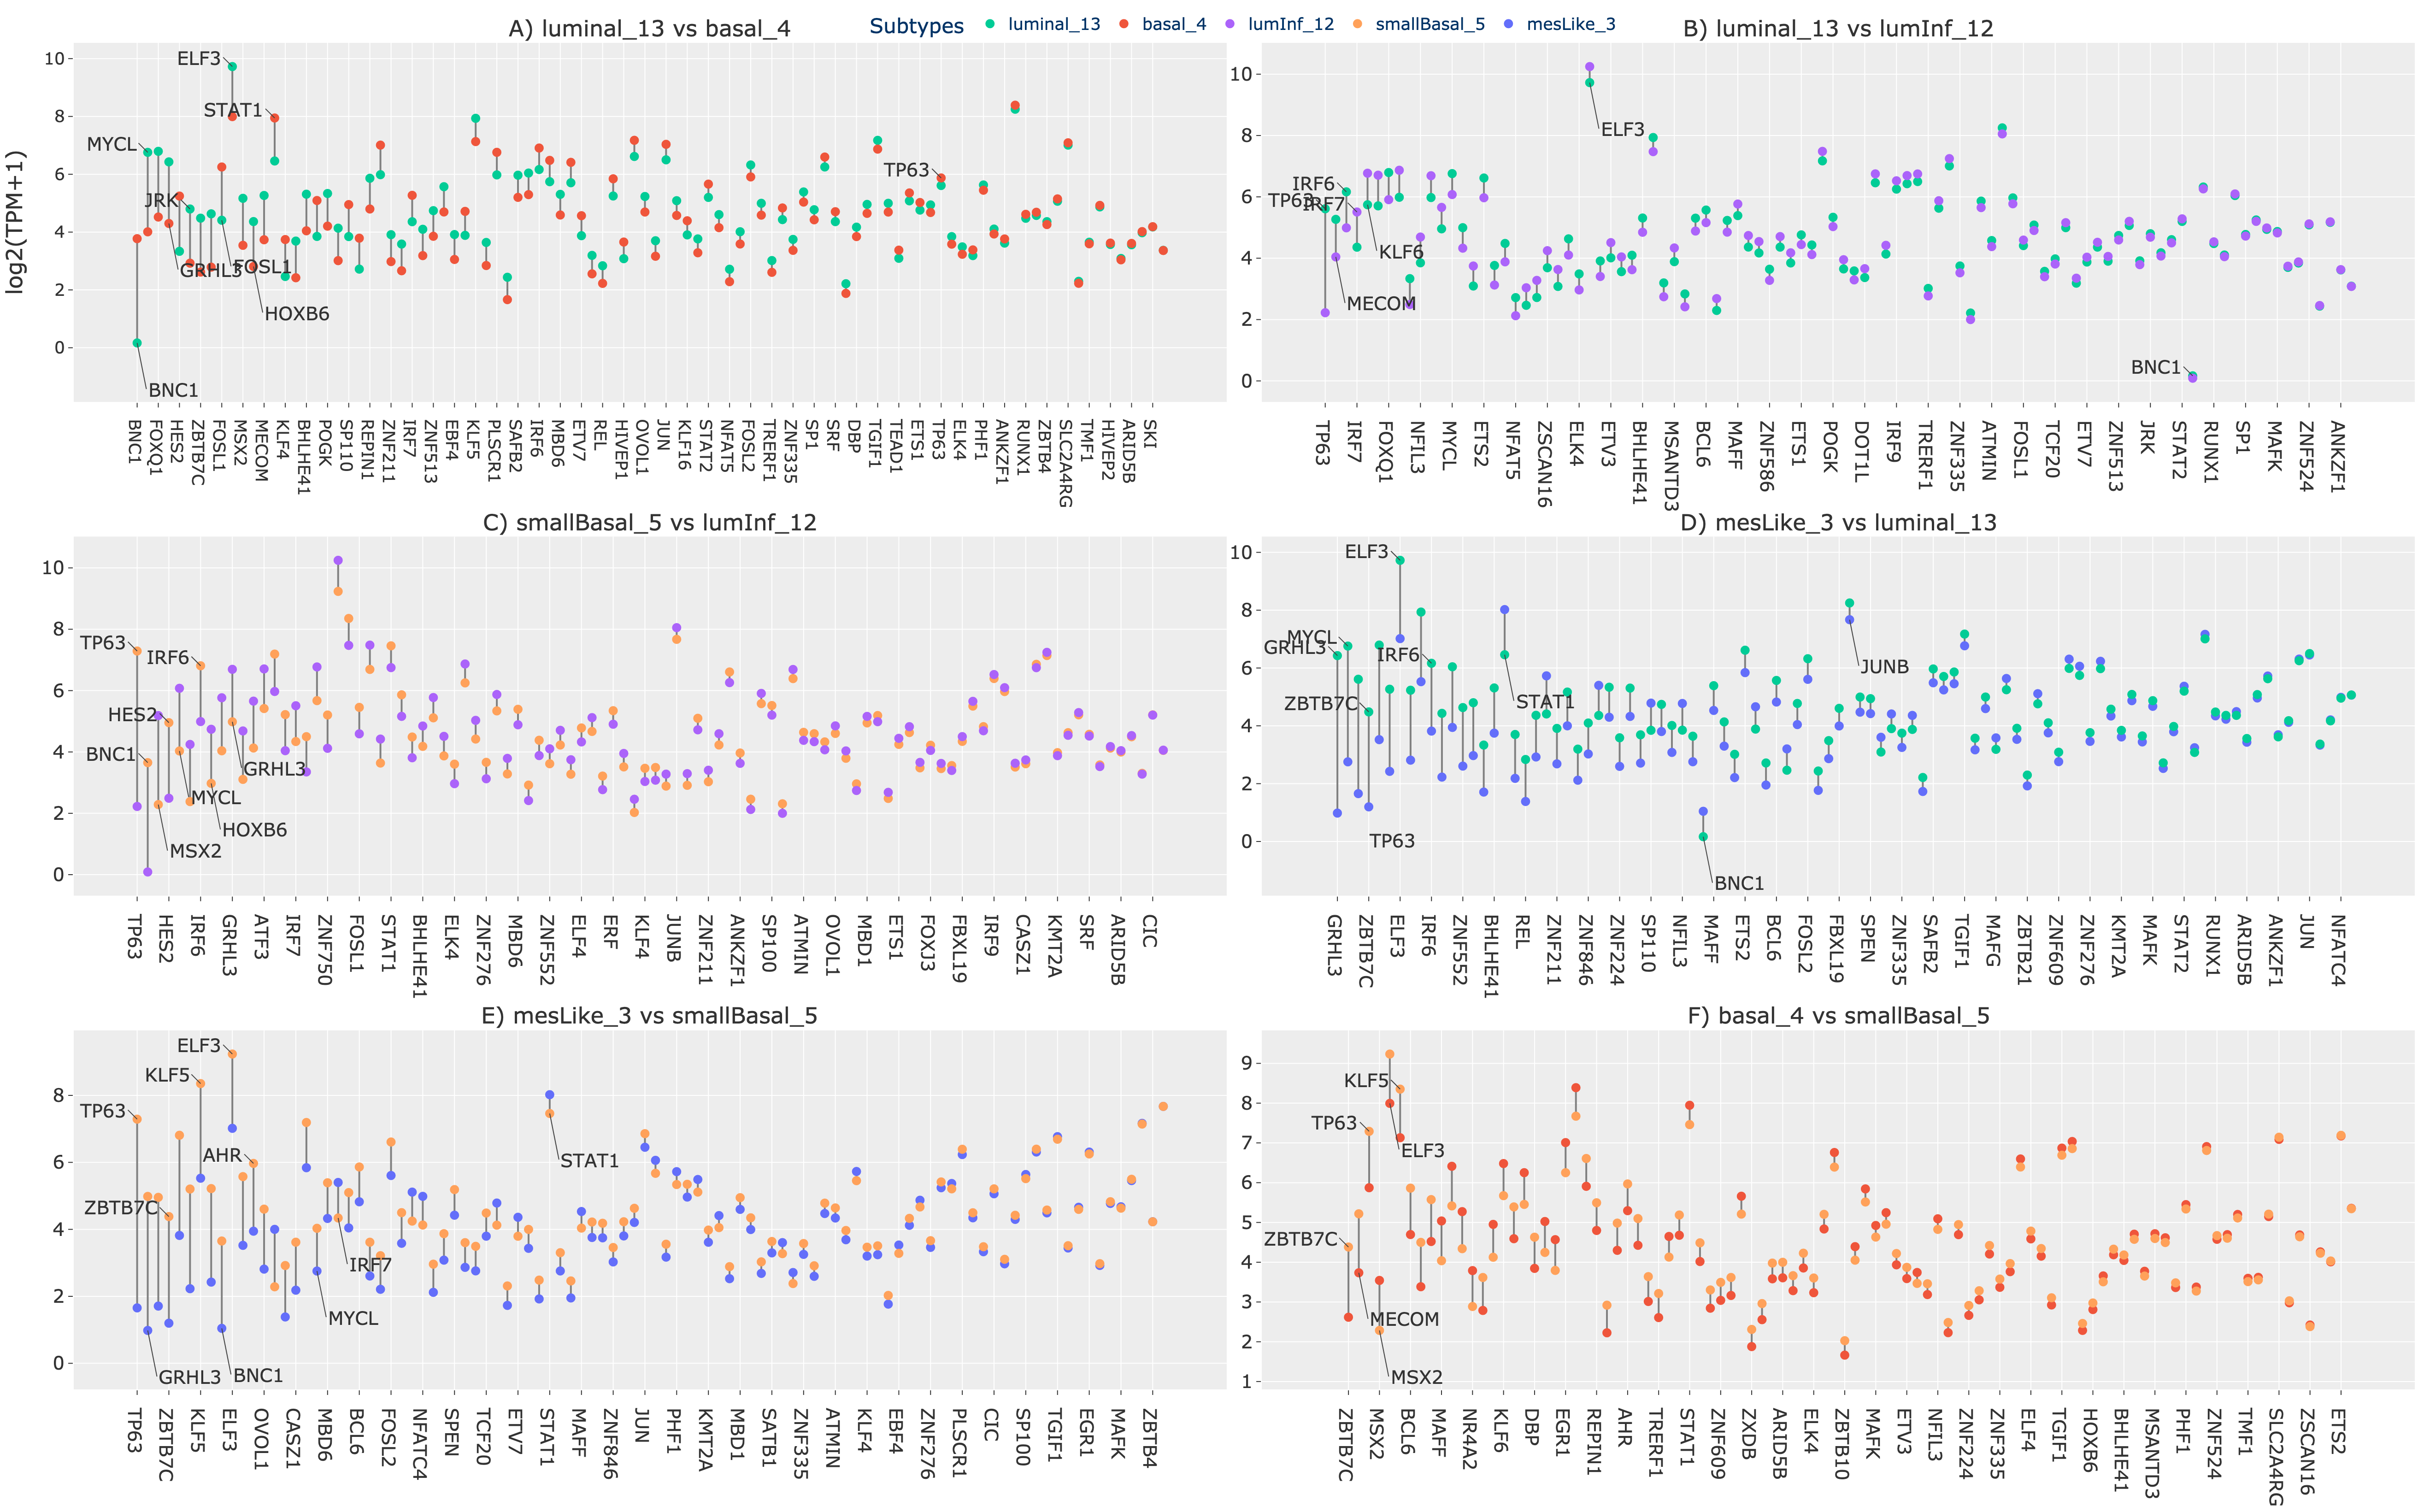
\includegraphics[width=1.0\textwidth,height=1.0\textheight,keepaspectratio]{Sections/Network_I/Resources/selective_pruning/dumbell_sel_tfs.png}
  \caption{Comparison of the mean across the subtypes derived with the 98 TFs. Each point represents the $log2(mean\_TPM+1)$ and the subplots are in descending order of the fold change.}
\label{fig:N_I:dumbell_sel_tfs}
\end{figure}


% the biggest change
The dumbbell figure in \cref{fig:N_I:dumbell_sel_tfs} exhibit the difference in expression between subgroups. Each point represents the $log2(mean\_TPM+1)$ and the subplots are in descending order of the fold change between the two averages. The largest changes happen between the basal-like (4,5) and luminal-like (13, 12) subgroups as well as between mes-like (3) \& basal-like groupsl; see A) and C). The least changes happen in B) where the main group of Luminal is compared with the 'infiltrated' version, exhibiting a change in magnitude of expression rather then a major difference.  \Cref{fig:N_I:dumbell_sel_tfs} A) and C) shows that \textit{BNC1} is absent in both Luminal groups. This gene also is low expressed in the basal subtypes comparison with the mes-like gorup in D) and E). \textit{BNC1} is a squamous cell marker as shown by the work of \citet{Hurst2022-sp}.

\textit{TP63} is a known Squamous marker \citet{Robertson2023-na} and indirectly of un-differentiation status. The difference in expression between subgroups is the most evident in the comparison of the basal subtypes (C and E) as well as in the small basal vs mes-like (C). The basal groups having higher mean expression than the others, with the highest in the small basal group (F). It is worth noting, that there is little fold change in the basal and luminal comparison (A). The basal groups over the mes-like are characterised by having a higher expression in: \textit{HES2, GRHL3, IRF6, ZNF750, BNC1, OVOL1, KLF5}. The smaller basal group seems to have stronger expression of the basal markers compared to the larger ones.

Overall, there are a few genes that have large changes in the comparison shown in \cref{fig:N_I:dumbell_sel_tfs}: 
\begin{itemize}
    \item \textit{BNC1, MYCL, FOXQ1, HES2, GRHL3 and HOXB6} in the main Basal (4), Luminal (13) comparison
    \item \textit{TP63} between Luminal (13) and Luminal infiltrated (12)
    \item \textit{TP63, BNC1, HES2, MSX2, MYCL, HOXB6, IRF6, GRHL3} - small Basal (5) and Luminal infiltrated (12), \textit{BNC1} being completely unexpressed in the subgroup 12
    \item \textit{TP63, HES2, GRHL3, IRF6, BNC1, ZNF750, ZBTB7C, MYCL} - mes-like (3) vs Basal (4), \textit{BNC1} being unexpressed in the mes-like group
    \item \textit{GRHL3, TP64, HES2, IRF6, ZBTB7C, ZNF750, BNC1, OVOL1} - mes-like (3) vs small Basal (5) 
    \item \textit{ZBTB7C, MECOM, MSX2, TP63, KLF5, ELF3} - large Basal (4) vs small Basal (5); this comparison shows that the smaller basal has higher enriched of basal markers.
\end{itemize}


It is know that \textit{MYCL, GRHL3, HOXB6, KLF5, ELF3} are involved in bladder differentiation, \textit{TP63} is a marker for undifferentiated and squamous tumours in MIBC as well as \textit{HES2}. The surprising TF is \textit{BNC1} which is completely un-expressed in the luminal tumours and expressed in the Basal subgroups; admittedly not very high as shown in \cref{fig:ap:sel_tfs_mean}. This suggests that many of the mentioned TFs may have a role in tissues differentiation.

This preliminary analysis of the differences in gene expression between subtypes indicates the presence of significant biological insights to be uncovered from the subgroups derived using the 98 TFs. This is further supported by the notable survival disparity observed in the small basal group, as shown in \cref{fig:N_I:sel_tfs_survival}. The subsequent section aims to refine the list of 98 TFs and to investigate the underlying biology of each MIBC subtype.

% Biological analysis
\subsection{The biology behind the emergent TFs} \label{s:N_I:sel_tfs_bio}

The bar plots in \cref{fig:N_I:sel_tfs_var} display the log mean of the gene expression in both non-cancerous and cancerous datasets of the 98 TFs genes. The error bars depict the standard deviation of expression and the genes are in the descending order of the tumour average expressions. The red-bars represent the genes have a high variance\footnote{In this case, a high varied genes is one which has a standard deviation as big as the mean expression} in the either the non-cancerous or tumour dataset and the golden are the genes varied in both. Highly varied genes are the ones highlighted in the bar plot may yield important gene expression markers between the subgroups. The three list of varied genes can be seen \cref{tab:N_I:sel_tfs_var}.

% Variance
\begin{figure}[!htb]   
\centering
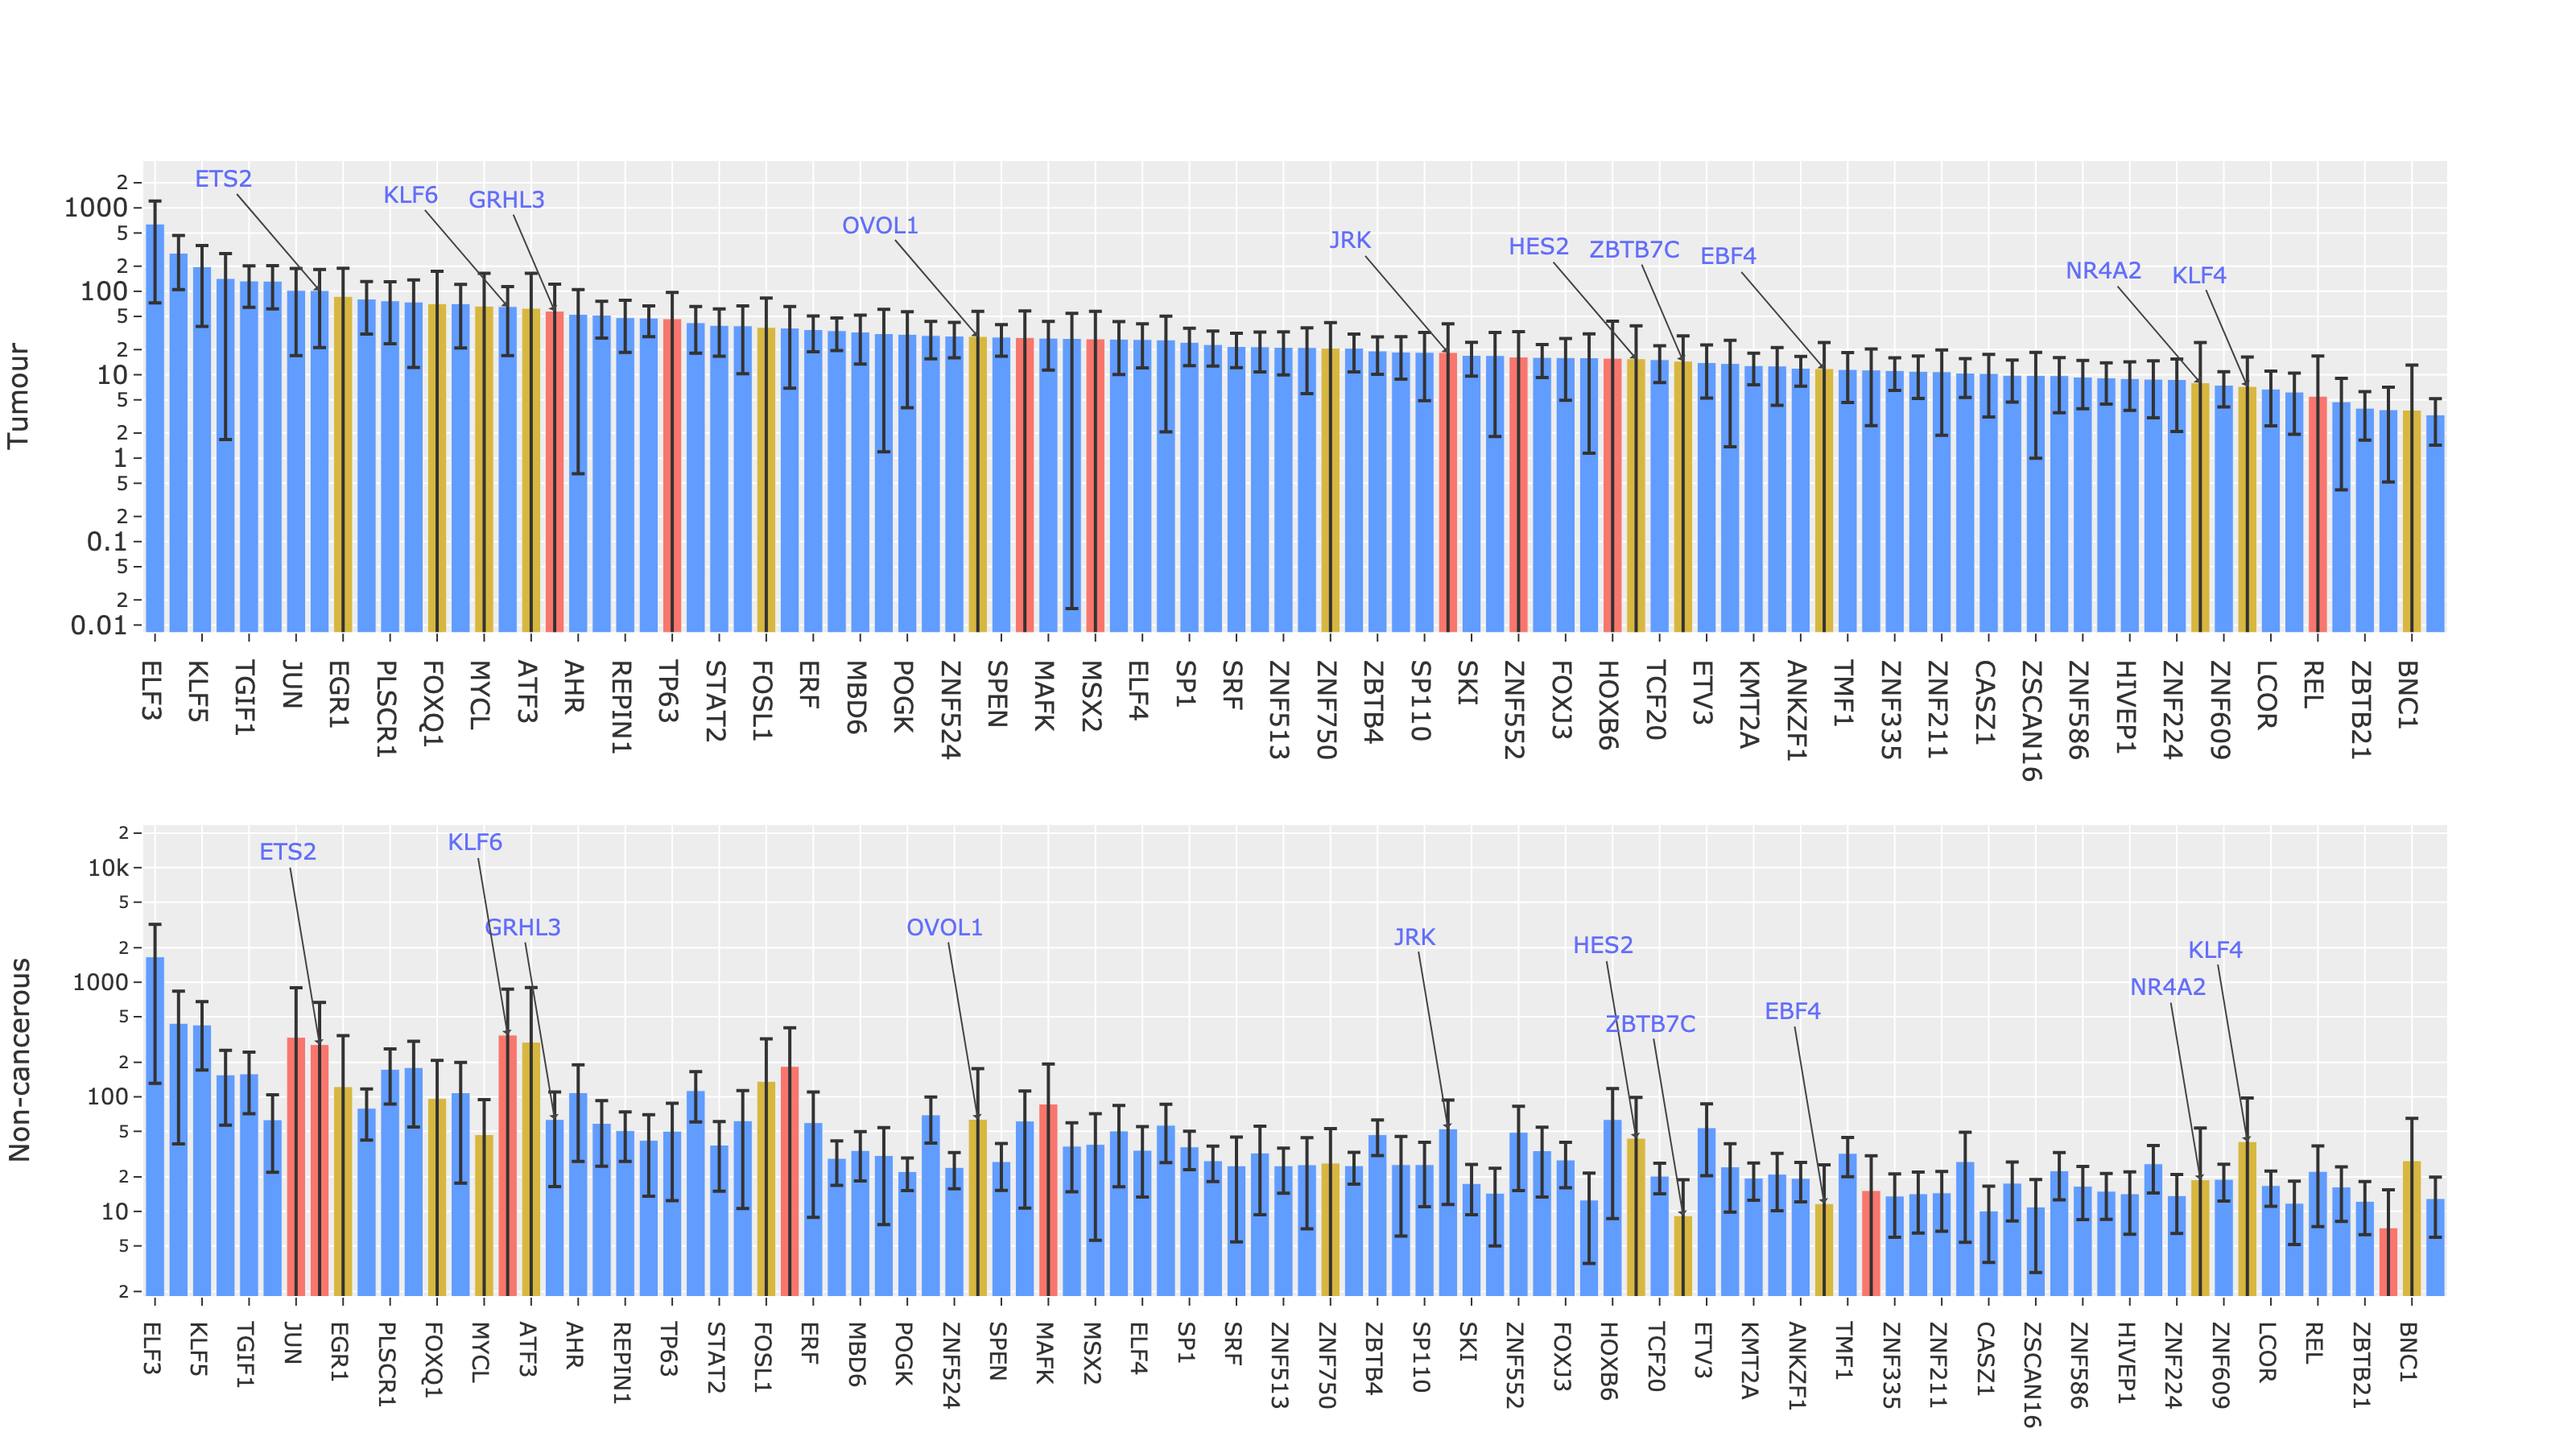
\includegraphics[width=1.0\textwidth,height=1.0\textheight,keepaspectratio]{Sections/Network_I/Resources/selective_pruning/sel_tfs_var_tum_healthy.png}
  \caption{Bar plot of the log mean expression in both non-cancerous and tumour datasets with the error bars accounting for standard deviation. The genes are ordered in descending order by the mean values in the non-cancerous dataset. Red bars represents genes that have a high variance in the corresponding dataset, while the golden shows the TFs in both tumour and non-cancerous.}
\label{fig:N_I:sel_tfs_var}
\end{figure}

There are few genes that are highly expressed in both the tumours and non-cancerous datasets such as \textit{ELF3, KLF5} or \textit{JUN}. A scatter plot version of the bar plot can be seen in \cref{fig:ap:sel_tfs_mean} from Appendix, where the x-axis represents the non-cancerous mean, y-axis the tum mean and the size and colour the mutation burden of the genes.

\begin{table}[H]
  \centering
  \scriptsize
  \begin{tabularx}{\textwidth}{>{\hsize=.25\hsize}X|>{\hsize=.75\hsize}X}
    \toprule
    \textbf{Category} & \textbf{Genes} \\
    \midrule
    Varied in Both & \textit{OVOL1, FOSL1, KLF4, BNC1, MYCL, NR4A2, ZBTB7C, FOXQ1, ZNF750, EGR1, HES2, ATF3, EBF4} \\
    \midrule
    Tumours only & \textit{BHLHE41, JRK, MSX2, TP63, ZNF552, GRHL3, HOXB6, REL} \\
    \midrule
    Non-cancerous only & \textit{ZBTB10, ARID5B, KLF6, JUN, MAFF, ETS2, MAFK} \\
    \bottomrule
  \end{tabularx}
    \caption{Gene Variation Across Sample Types} % Caption for the table
    \label{tab:N_I:sel_tfs_var}
\end{table}

It is worth remembering that MIBC is generally divided into Luminal and Basal subgroups, the former exhibiting differentiated status, while the latter an undifferentiated status. The non-cancerous dataset contains samples that are either differentiated (Abs-Ca or in-situ) or undifferentiated. This implies that the TFs with a high mean deviation may play a role in differentiation and also help in understanding the Basal/Luminal differences in MIBC. The molecular particularities in the tissue types of differentiation tissues are next explored.


% Undiff vs Diff
\subsection*{The emergent TFs and bladder differentiation} \label{s:N:sel_tf_diff_status}

\begin{figure}[!h]
    \captionsetup[subfigure]{justification=Centering}
\begin{subfigure}[!t]{1.0\textwidth}
    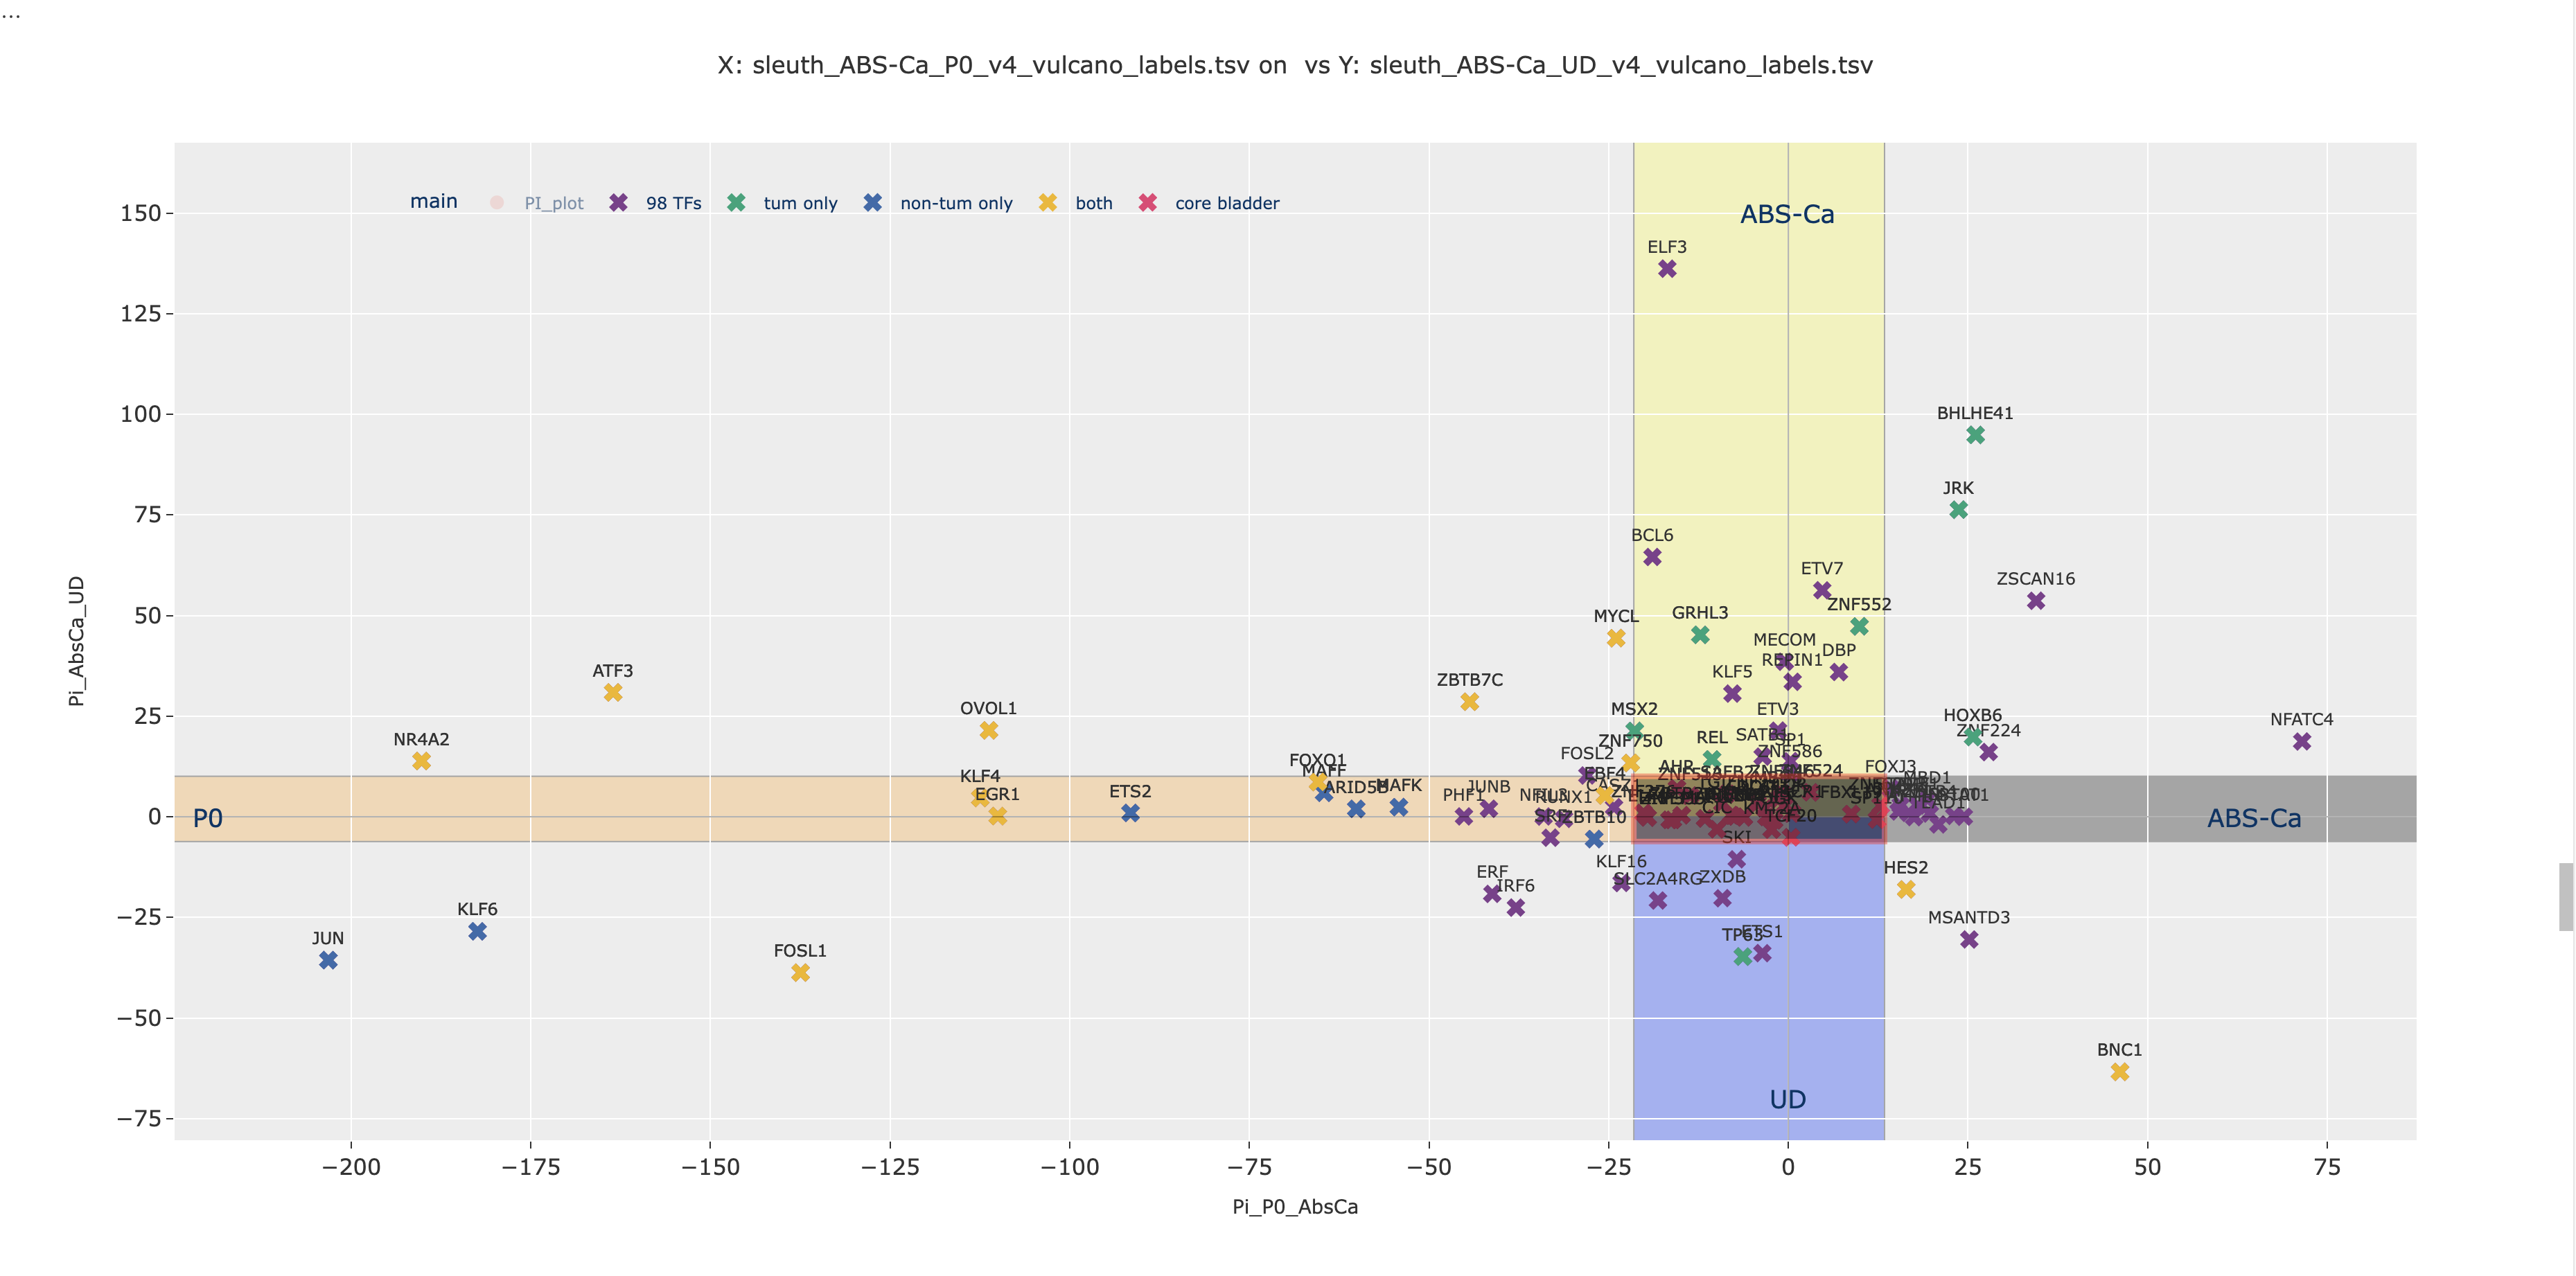
\includegraphics[width=1.0\textwidth,height=1.0\textheight,keepaspectratio]{Sections/Network_I/Resources/selective_pruning/sel_tfs_pi_all_var_rect.png}
    
    \caption{Pi plot with just the varied genes}
    
    \label{fig:N_I:pi_sel_tfs_var}
\end{subfigure}\hspace{\fill} % maximize horizontal separation

\begin{subfigure}[!t]{1.0\textwidth}
    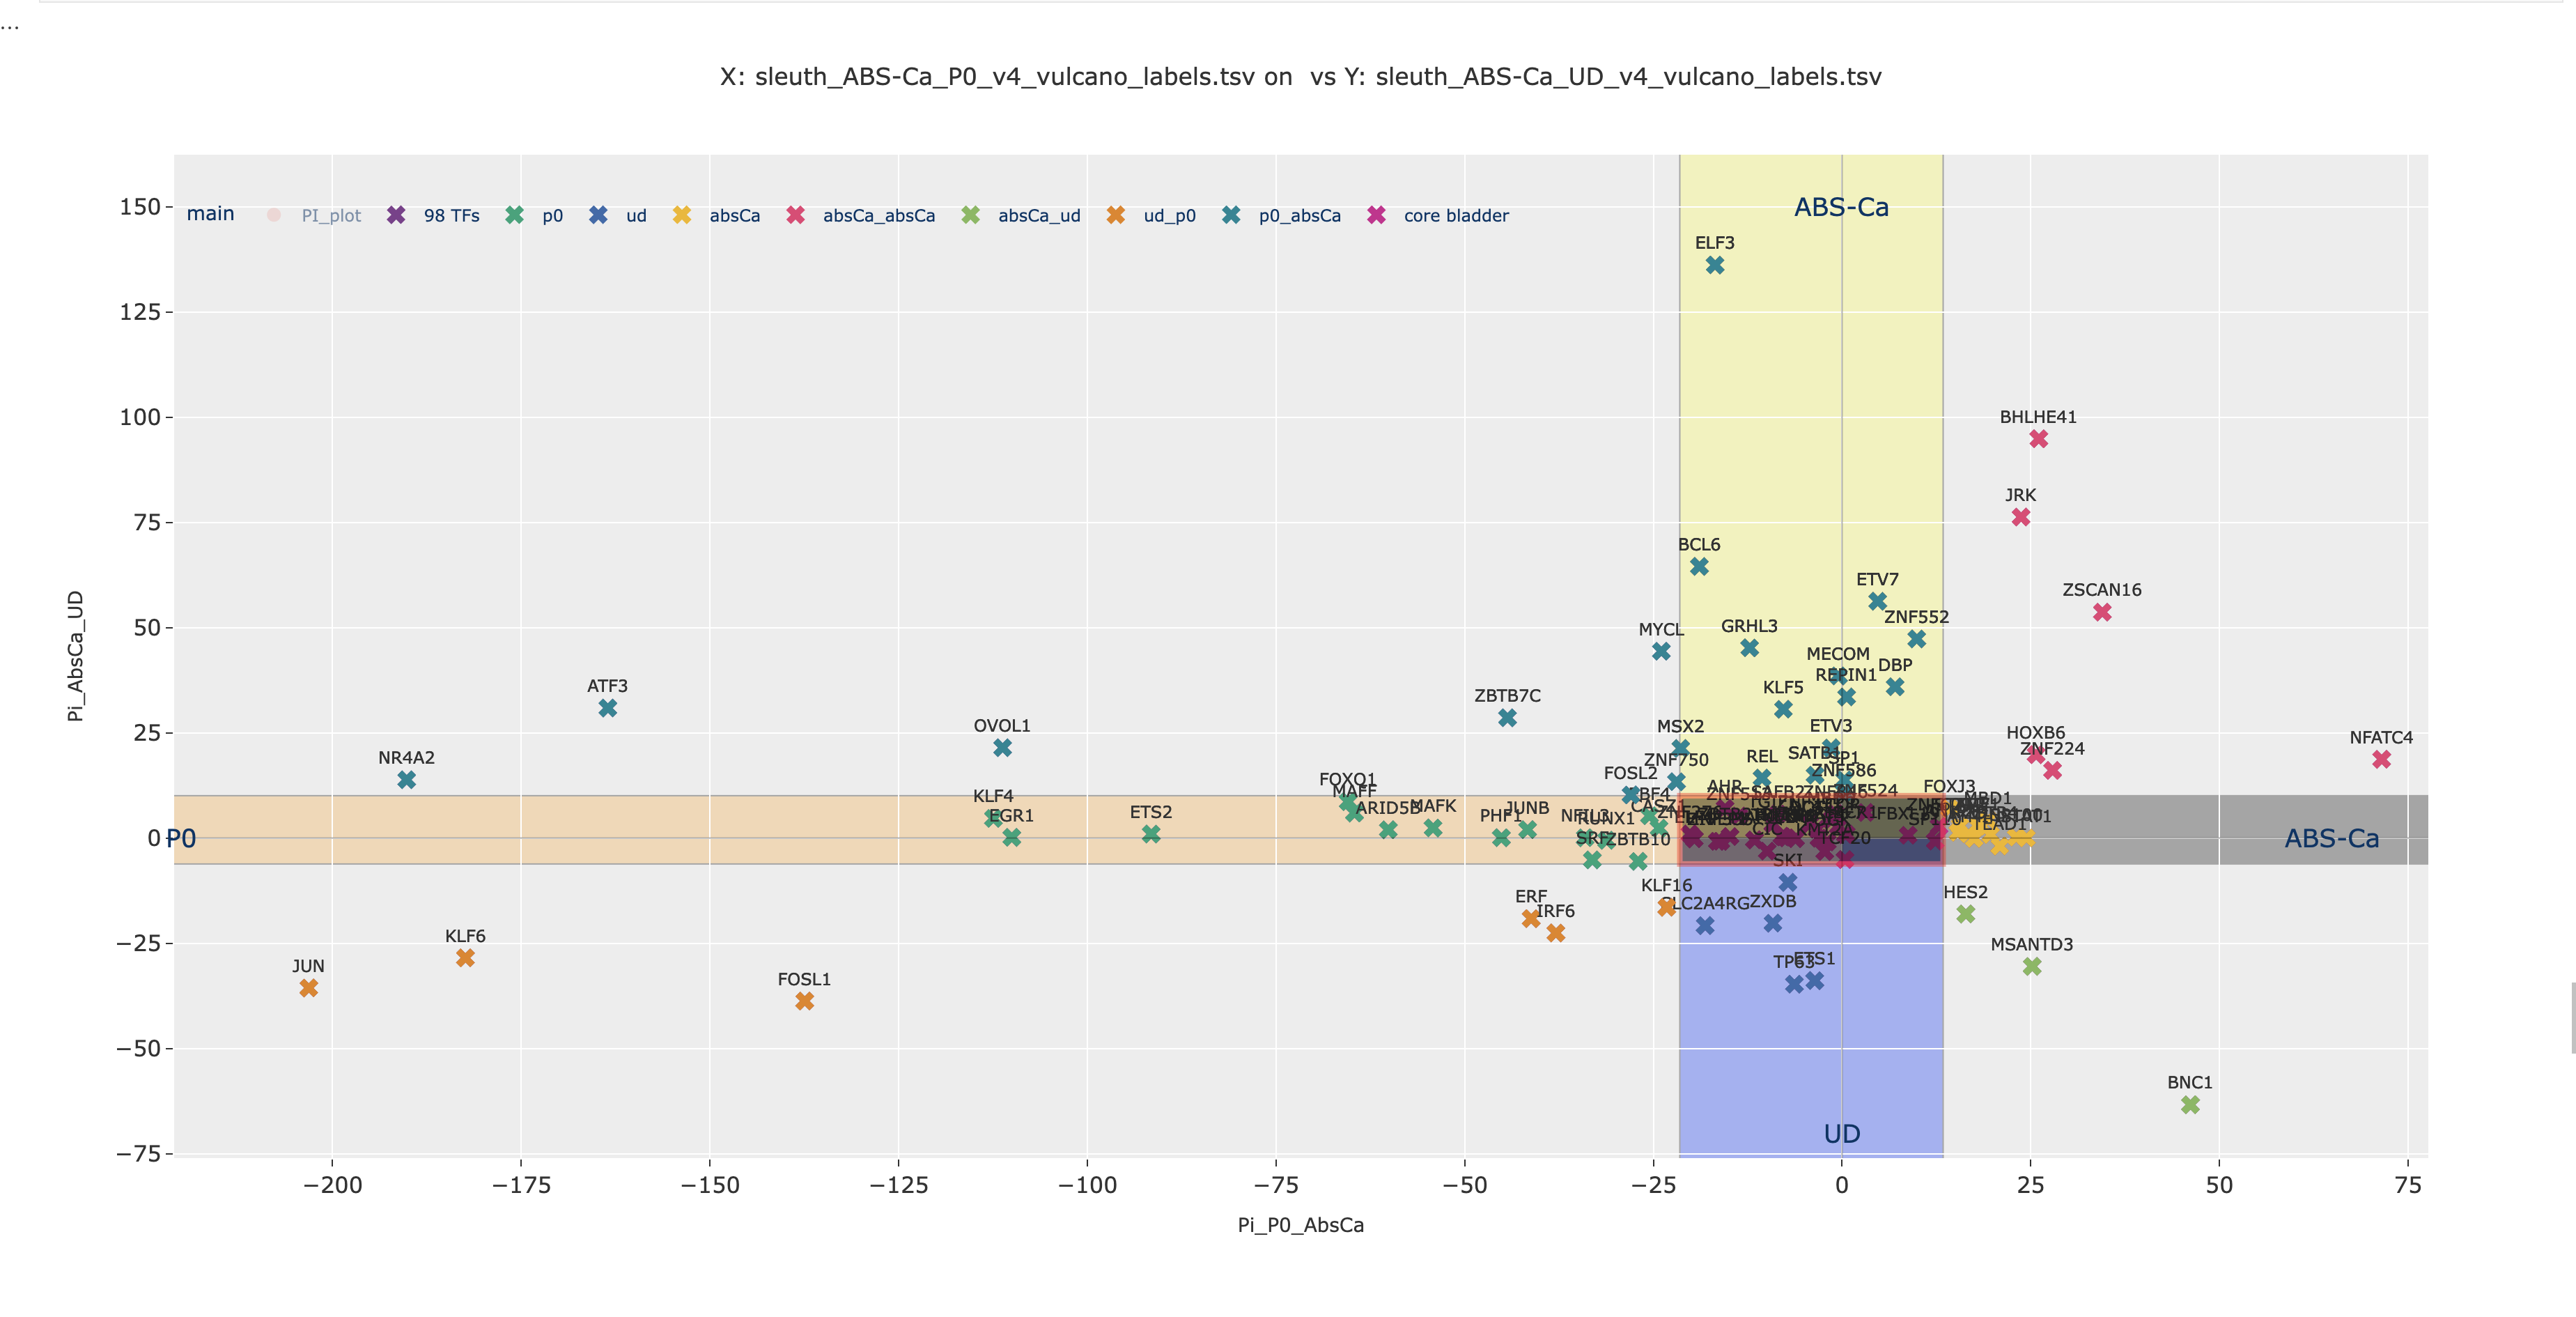
\includegraphics[width=1.0\textwidth,height=1.0\textheight,keepaspectratio]{Sections/Network_I/Resources/selective_pruning/sel_tfs_pi_all_tissueDiff.png}
    
    \caption{Pi plot with all the 98 TFs}
    
    \label{fig:N_I:pi_sel_tfs_all}
\end{subfigure}\hspace{\fill} % maximize horizontal separation

    \caption{Two Pi plots of the same comparisons, but with different markers shown. The X-axis represents the Pi values from the DEA of the P0 vs AbsCa, the Y-axis from AbsCa vs UD. The markers yellow are the most varied genes seen in \cref{fig:N_I:sel_tfs_var}, the blue the genes highly varied only in the non-cancerous where the green highly varied in the tumour. The rest of the markers in purple are rest of the 98 TFs gene.}
    
    \label{fig:N_I:pi_sel_tfs}
\end{figure}

% Introducing the two pi-plots
The pi plot in \cref{fig:N_I:pi_sel_tfs} presents the 98 TFs in the context of the non-cancerous tumour dataset from the JBU. The Y coordinate is given by the pi value (-$log10(q)*fold\_change$) from the DEA performed between the Undifferentiated (UD) and Abs-Calcium (AbsCa) group, where the X-coordinate is the comparison between AbsCa and P0 (in-situ). The positive values on the Y-axis represents the ABS-Ca specific TF, while the negative values the genes closed to UD. Where the negative values on the X-axis are P0 specific and conversely for the positive values and AbsCa. The rectangles are drawn  within $+/-5\%$ of the axes and are a visual cue for the genes that are very close to the axis. These are different scales as the pi values across comparison has different ranges. This difference in axes ranges needs to be accounted for when interpreting the plot, especially in the UD - P0 quadrant. 

% Just the sel tfs - UD and P0
In \cref{fig:N_I:pi_sel_tfs}, it can be seen that \textit{BNC1} and \textit{HES2} are UD markers, which may also indicate specificity for squamous markers. \textit{TP63} is another squamous marker \cite{Robertson2017-mg}, but it is more significantly differentiated in the UD vs Abs-Ca comparison. \textit{FOSL1} is a highly varied gene that appears to be both an undifferentiated and P0 marker (note the difference in scale between the X-axis and Y-axis). \textit{KLF6} and \textit{JUN} are genes more specific to P0 but are also highly expressed in the undifferentiated tissue.


% Talk about the differentiation markers 
The two Y-positive quadrants contains the genes that are likely involved in the differentiation of the bladder tissue, closer to the x-axis, more specific to the culture mode, conversely to Y-axis to the P0. It is worth noting that most of the genes specific to Abs-Ca model are highly varied in the tumours, which may suggest that are more expressed in the Luminal tumours compared to the Basal; \textit{HOXB6, ZNF552, JRK, BHLHe41}. Genes \textit{ZNF750, MSX2, MYCL, GRHL3 and REL} are specific to both P0 and Abs-Ca. Both \textit{MYCL, GRHL3} are known to be differentiation markers. There are also markers that are specific to P0 samples: \textit{EBF4, MAFK, ARID5B, EGR1, ETS2, MAFF, FOX1, KLF4, NR4A2, ATF3, OVOL1}. 

While \cref{fig:N_I:pi_sel_tfs_var} offer a focused view on the TFs that are varied in the non-cancerous and/or the MIBC cohort from TCGA, \cref{fig:N_I:pi_sel_tfs_all} complements the plot by showing all the 98 TFs. It can be noticed that there are several markers that might be UD specific (negative X-axis) while some additional markers involved in differentiation which do not vary as much. The latter may suggest that these markers are common both in Basal and Luminal tumours. 

% No TFs shared between UD and Abs-Ca
It is surprising that there are no TFs shared in the culture quadrant (UD and Abs-Ca) and many TFs in the middle of the Pi plot. The genes at the centre of the pi plot may indicate a list of TFs that are at the core of bladder tissue, regardless if it is differentiated or undifferentiated.

\begin{table}[H]
  \centering
  \scriptsize
  \begin{tabularx}{\textwidth}{>{\hsize=.15\hsize}X|>{\hsize=.85\hsize}X}
    \toprule
    \textbf{Category} & \textbf{Genes} \\
    \midrule
    \textbf{P0} & \textit{KLF4, ETS2, PHF1, ARID5B, EGR1, FOXQ1, MAFF, JUNB, MAFK, NFIL3, SRF, RUNX1, CASZ1, ZBTB10, EBF4} \\
    \midrule
    \textbf{UD} & \textit{SLC2A4RG, ZXDB, SKI, TP63, ETS1} \\
    \midrule
    \textbf{AbsCa} & \textit{BCL6, MSX2, ELF3, GRHL3, REL, KLF5, ZNF552, SATB1, DBP, ETV7, ETV3, MECOM, REPIN1, SP1, ZNF586, ZBTB4, TEAD1, ATMIN, TMF1, SP100, FOXJ3, MBD1, STAT1, ANKZF1, IRF9, STAT2, NFATC4, ZNF224, ZSCAN16, JRK, BHLHE41, HOXB6} \\
    \midrule
    \textbf{AbsCa-UD} & \textit{BNC1, MSANTD3, HES2} \\
    \midrule
    \textbf{UD-P0} & \textit{KLF6, JUN, FOSL1, ERF, IRF6, KLF16} \\
    \midrule
    \textbf{P0-AbsCa} & \textit{NR4A2, ATF3, OVOL1, ZBTB7C, FOSL2, BCL6, MSX2, MYCL, ZNF750, ELF3, GRHL3, REL, KLF5, ZNF552, SATB1, DBP, ETV7, ETV3, MECOM, REPIN1, SP1, ZNF586} \\
    \bottomrule
  \end{tabularx}
  \caption{TF marker classified by being significantly expressed in the two DEA comparisons: P0 vs AbsCa and UD vs AbsCa in \cref{fig:N_I:pi_sel_tfs}.} 
  \label{tab:N_I:markers_diff}
\end{table}

\Cref{tab:N_I:markers_diff} summarises the TF classification based on the differentiation tissue type: AbsCa (differentiation in culture), P0 (differentiation in tissue) and undifferentiated (culture). The 'transitional' genes in AbsCa-UD, UD-P0 and P0-AbsCa may yield information about the common genes shared between differentiation tissue types.


% Transitioning to cancer
\subsubsection*{The emergent TFs and cancer} \label{s:N_I:sel_tfs_cancer}


% Selecting the genes for basal and luminal, expression in both Basal and Luminal
Using the above work and the box plots like the ones in \cref{fig:N_I:box_basal,fig:N_I:box_luminal}, two lists of genes specific to Basal/Squamous (Ba/Sq) and Luminal subtypes were created, as shown in \cref{tab:N_I:genes_lum_basal}. A recent study by \citet{Ramal2024-ha}, which investigated the regulatory network in urothelial cells, concluded that the following genes are considered 'novel putative TFs' for luminal differentiation: \textit{\textbf{BHLHE41}, \textbf{MECOM}, \textbf{MYCL}, NCOA1, NR2F2, NR2F6, \textbf{REPIN1}, SREBF1, TBX2, TBX3, TRAFD1, and \textbf{ZBTB7C}}. The bold genes are among the 98 TFs identified in this section, while \textit{MECOM, BHLHE41, ZBTB7C} are selected as markers in \cref{tab:N_I:genes_lum_basal}. \textit{GRHL3} is also mentioned in the work by \citet{Ramal2024-ha}, but it has already been determined as a differentiation marker \citet{Bock2014-zy}. \citet{Chen2021-tc} studied the role of \textit{ZBTB7C} across different cancers and its relation to tumour mutational burden, microsatellite instability, and immune cell infiltration.

% Lum-basal markers
\begin{table}[!htb]
  \centering
  \scriptsize
  \begin{tabularx}{\textwidth}{>{\hsize=.25\hsize}X|>{\hsize=.75\hsize}X}
    \toprule
    \textbf{Category} & \textbf{Genes} \\
    \midrule
    \textbf{Luminal} & \textit{MSX2, HOXB6, MECOM, GRHL3, JRK, BHLHE41, ZBTB7C, ZSCAN16, ZNF224, ZBTB10} \\
    \midrule
    \textbf{Basal/Squamous} & \textit{TP63, BNC1, HES2, ERF, IRF6, ZXDB, ZNF750, ETS1, MSANTD3, FOSL1, KLF6, KLF16} \\
    \bottomrule
  \end{tabularx}
  \caption{The 98 transcription factors markers categorised by Luminal and Basal subtypes.} % Caption for the table
  \label{tab:N_I:genes_lum_basal}
\end{table}

% Discuss Squamous work
\citet{Hurst2022-sp} researched the upregulated and downregulated genes involved in the formation of squamous cell carcinoma (SCC), an undifferentiated tissue. Figure 4 from their paper shows the signature genes involved in this process. Among the upregulated genes in \citet{Hurst2022-sp}, the following are found in the 98 TFs: \textit{\textbf{BNC1}, EGR1, \textbf{FOSL1}, \textbf{HES2}, JUN, \textbf{KLF16}, KLF4, NFIL3}. From the list of downregulated genes, the following are found in the 98 TFs: \textit{\textbf{BHLHE41}, ELF3, FOXQ1, \textbf{MECOM}, POGK, REPIN1, ZSCAN16}. The bold genes are the markers chosen as markers for basal and luminal (\cref{tab:N_I:genes_lum_basal}).


% % Basal Markers 
\begin{figure}[H]
    \captionsetup[subfigure]{justification=Centering}
    % consensus
    \begin{subfigure}[!t]{0.49\textwidth}
        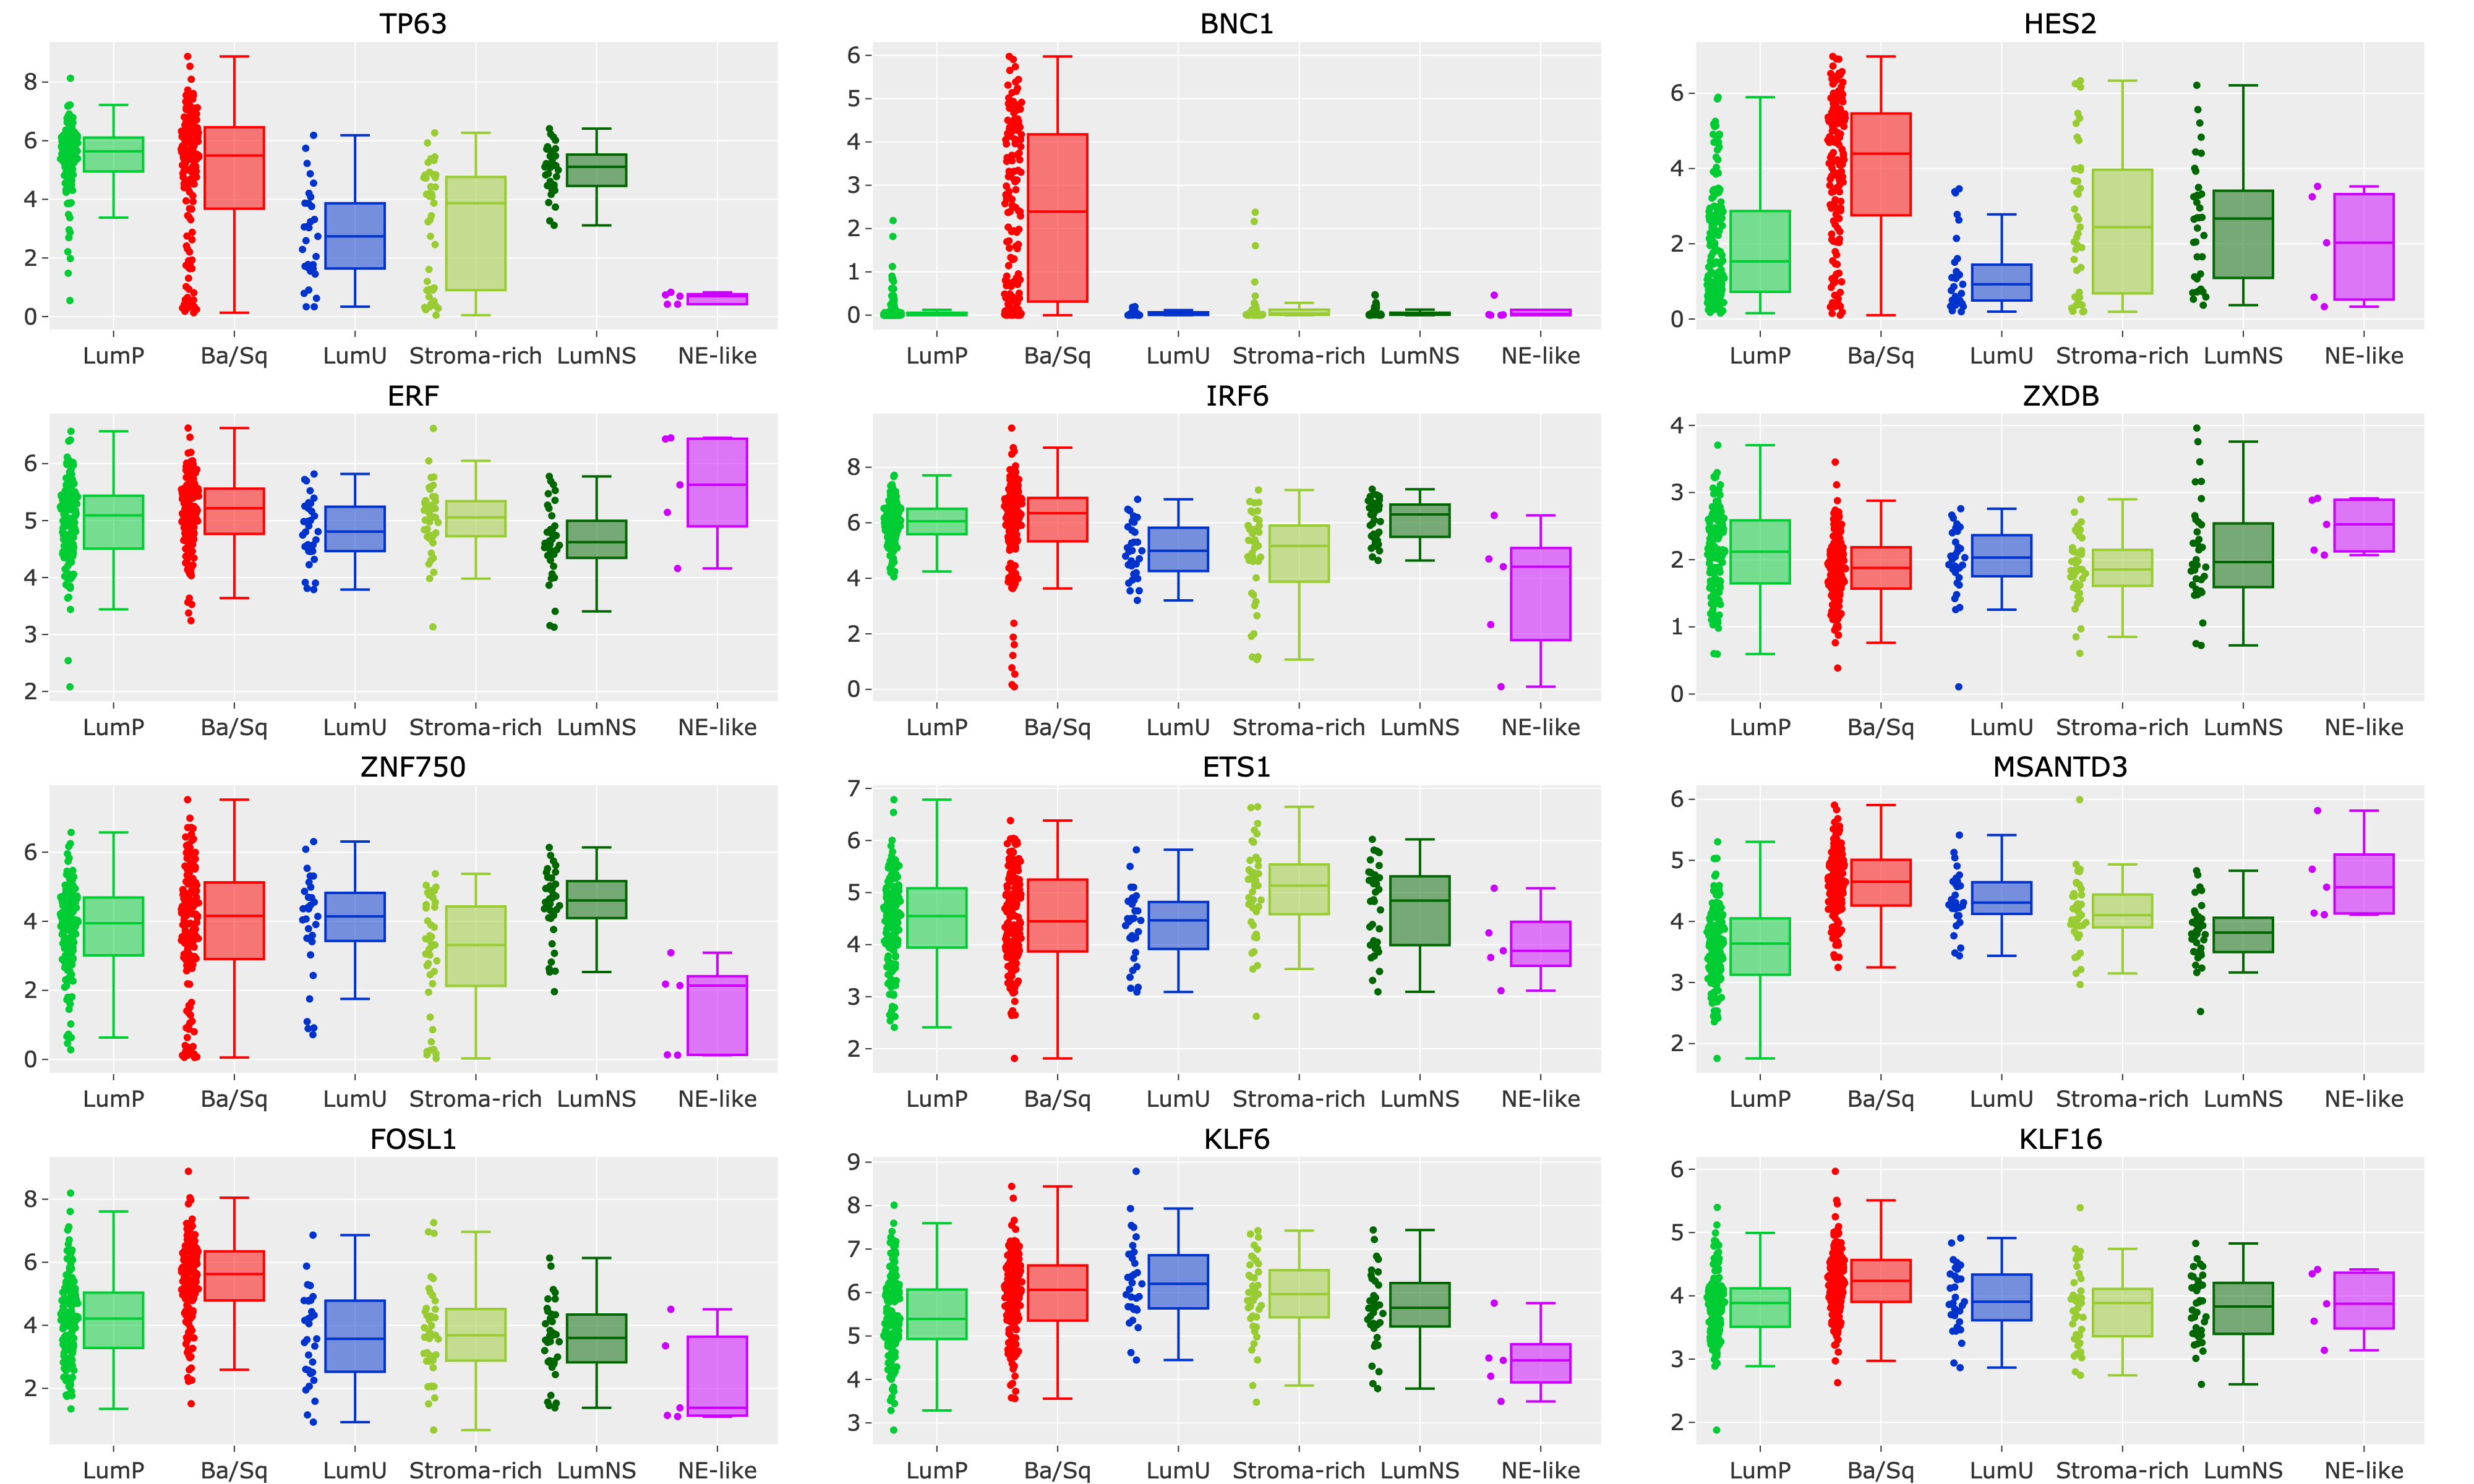
\includegraphics[width=1.0\textwidth,height=1.0\textheight,keepaspectratio]{Sections/Network_I/Resources/selective_pruning/log2_consensus_basal.png}
        \caption{Consensus}
        \label{fig:N_I:box_basal_consensus}
    \end{subfigure}
    \begin{subfigure}[!t]{0.49\textwidth}
        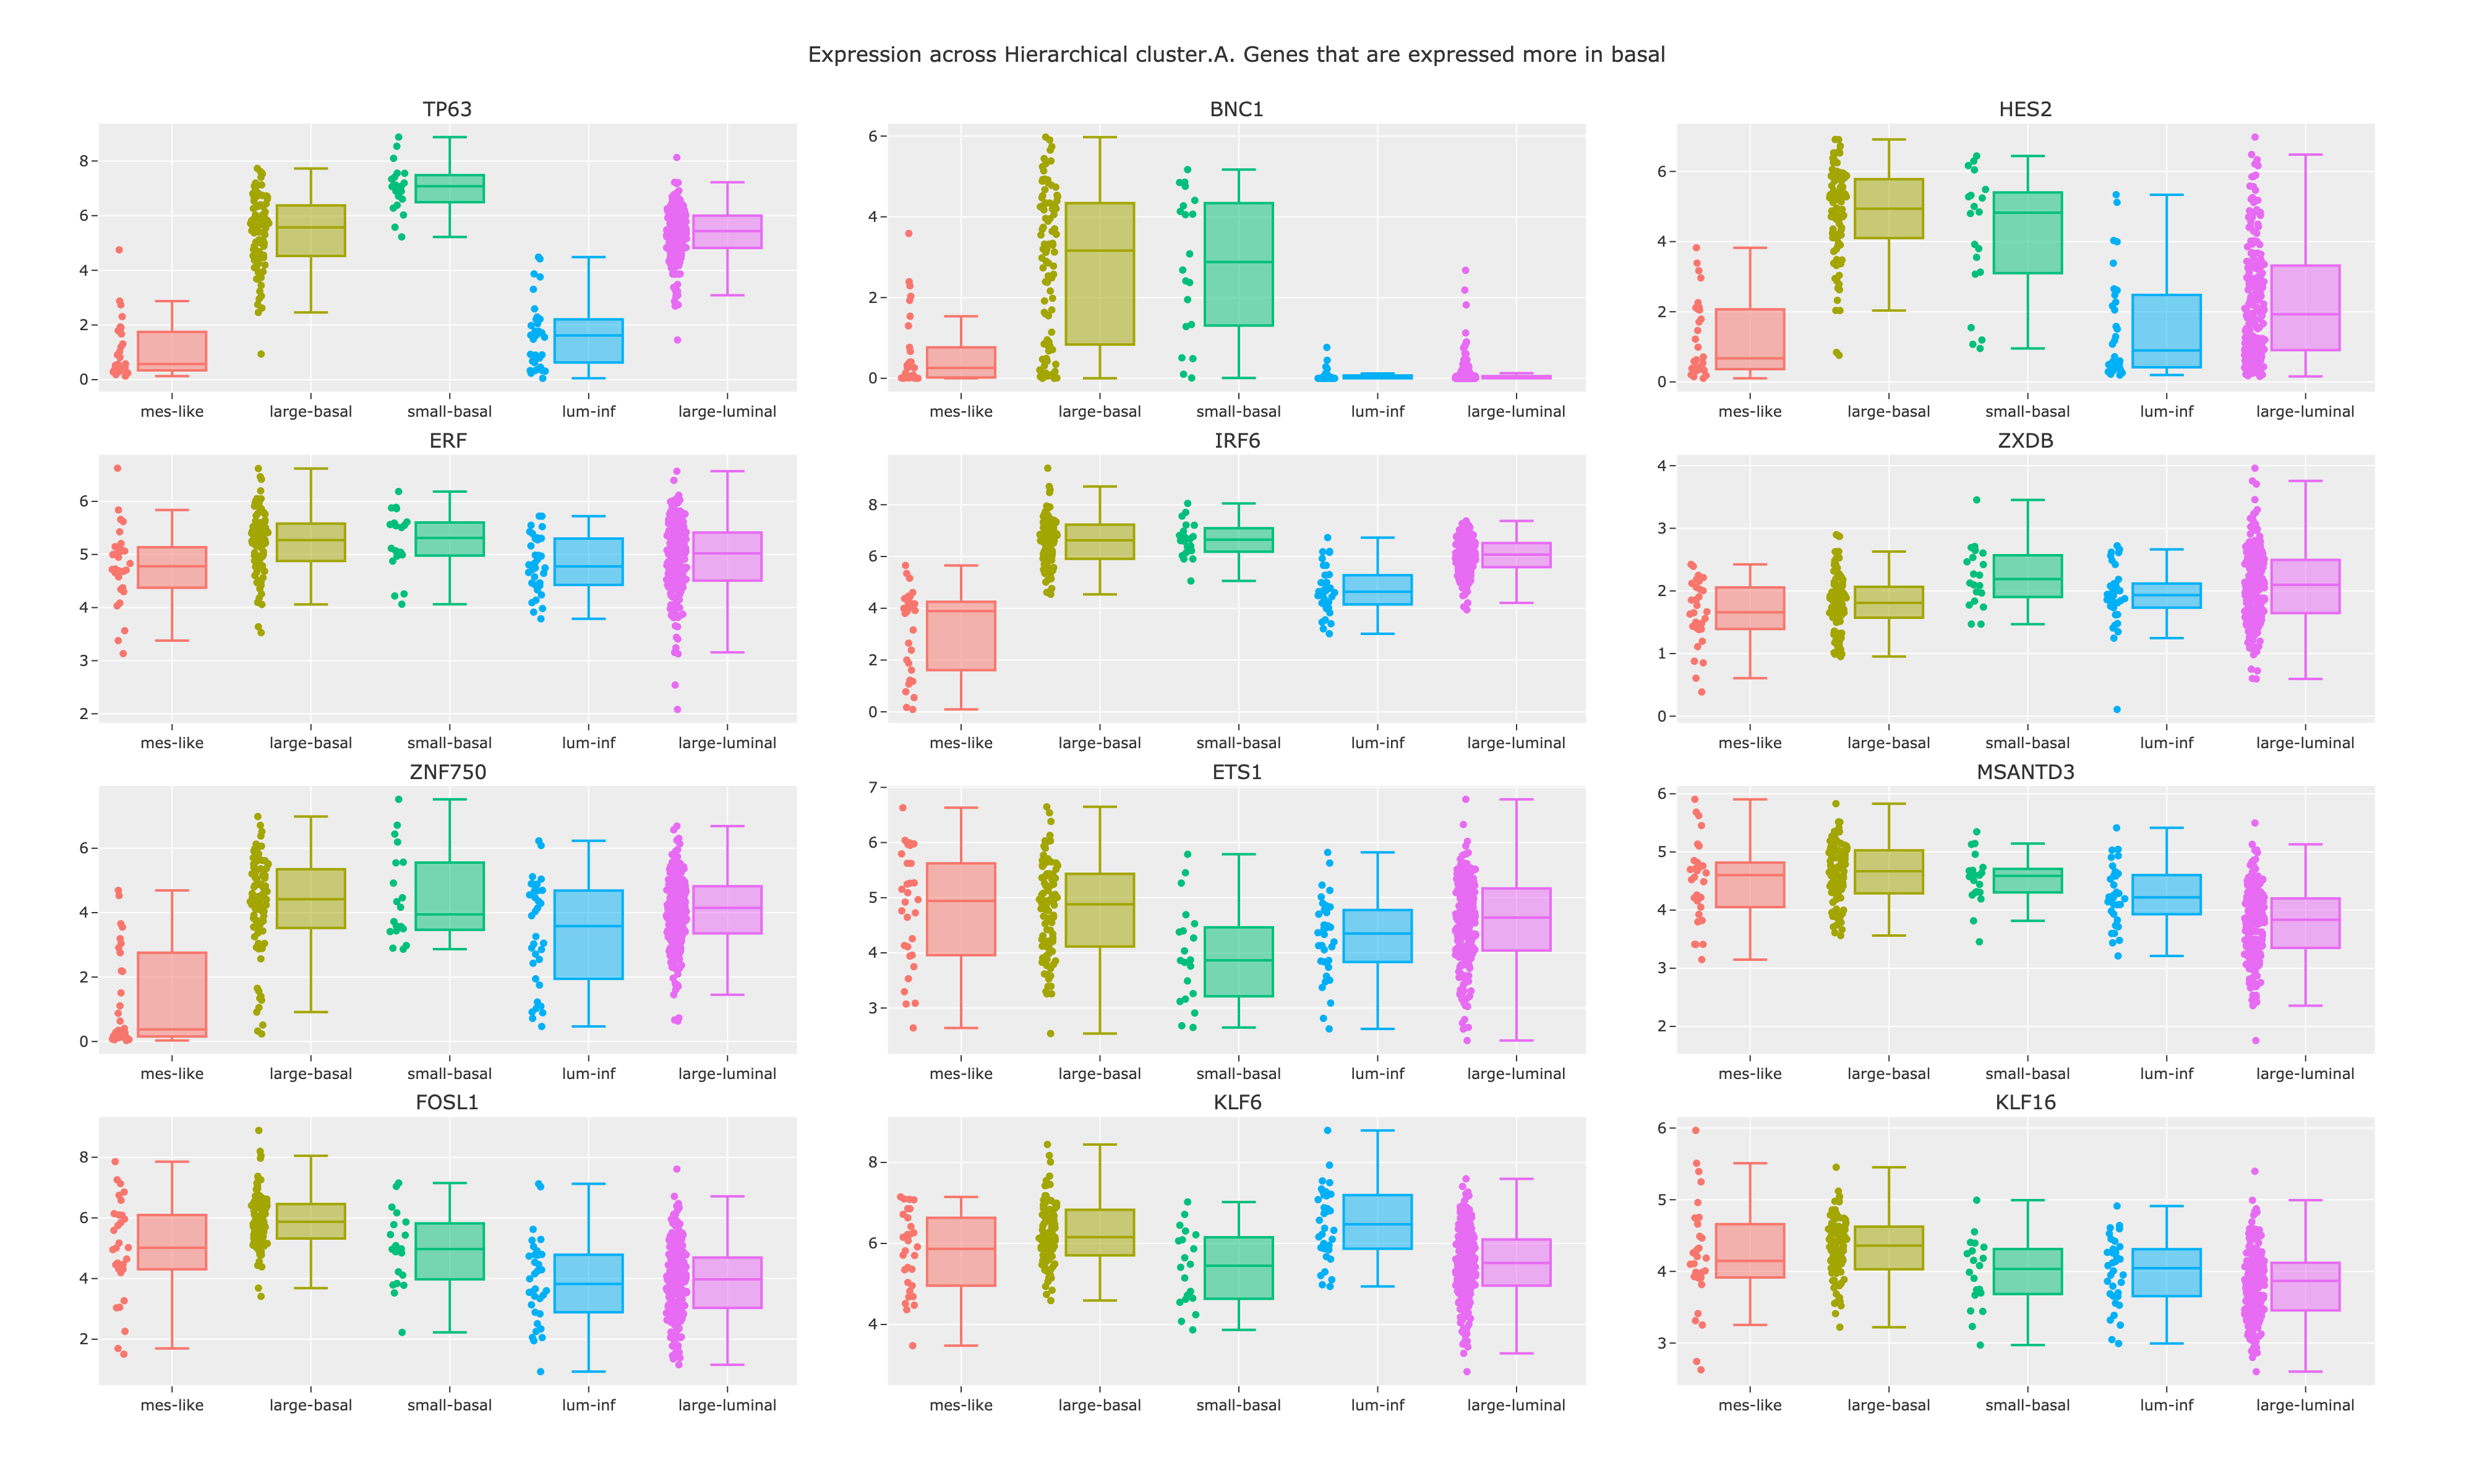
\includegraphics[width=1.0\textwidth,height=1.0\textheight,keepaspectratio]{Sections/Network_I/Resources/selective_pruning/log2_dendrogram_basla.png}
        \caption{Basal}
        \label{fig:N_I:box_basal_dendrogram}
    \end{subfigure}
    \caption{Box plots showing the $log2(TPM+1)$ of the \textbf{basal} markers over the consensus and groups derived from the hierarchical clustering applied in this chapter.}
    \label{fig:N_I:box_basal}
\end{figure}


% \begin{sidewaysfigure}[H]
%   \centering
%   % consensus
%   \begin{subfigure}[!t]{1.0\textwidth}
%       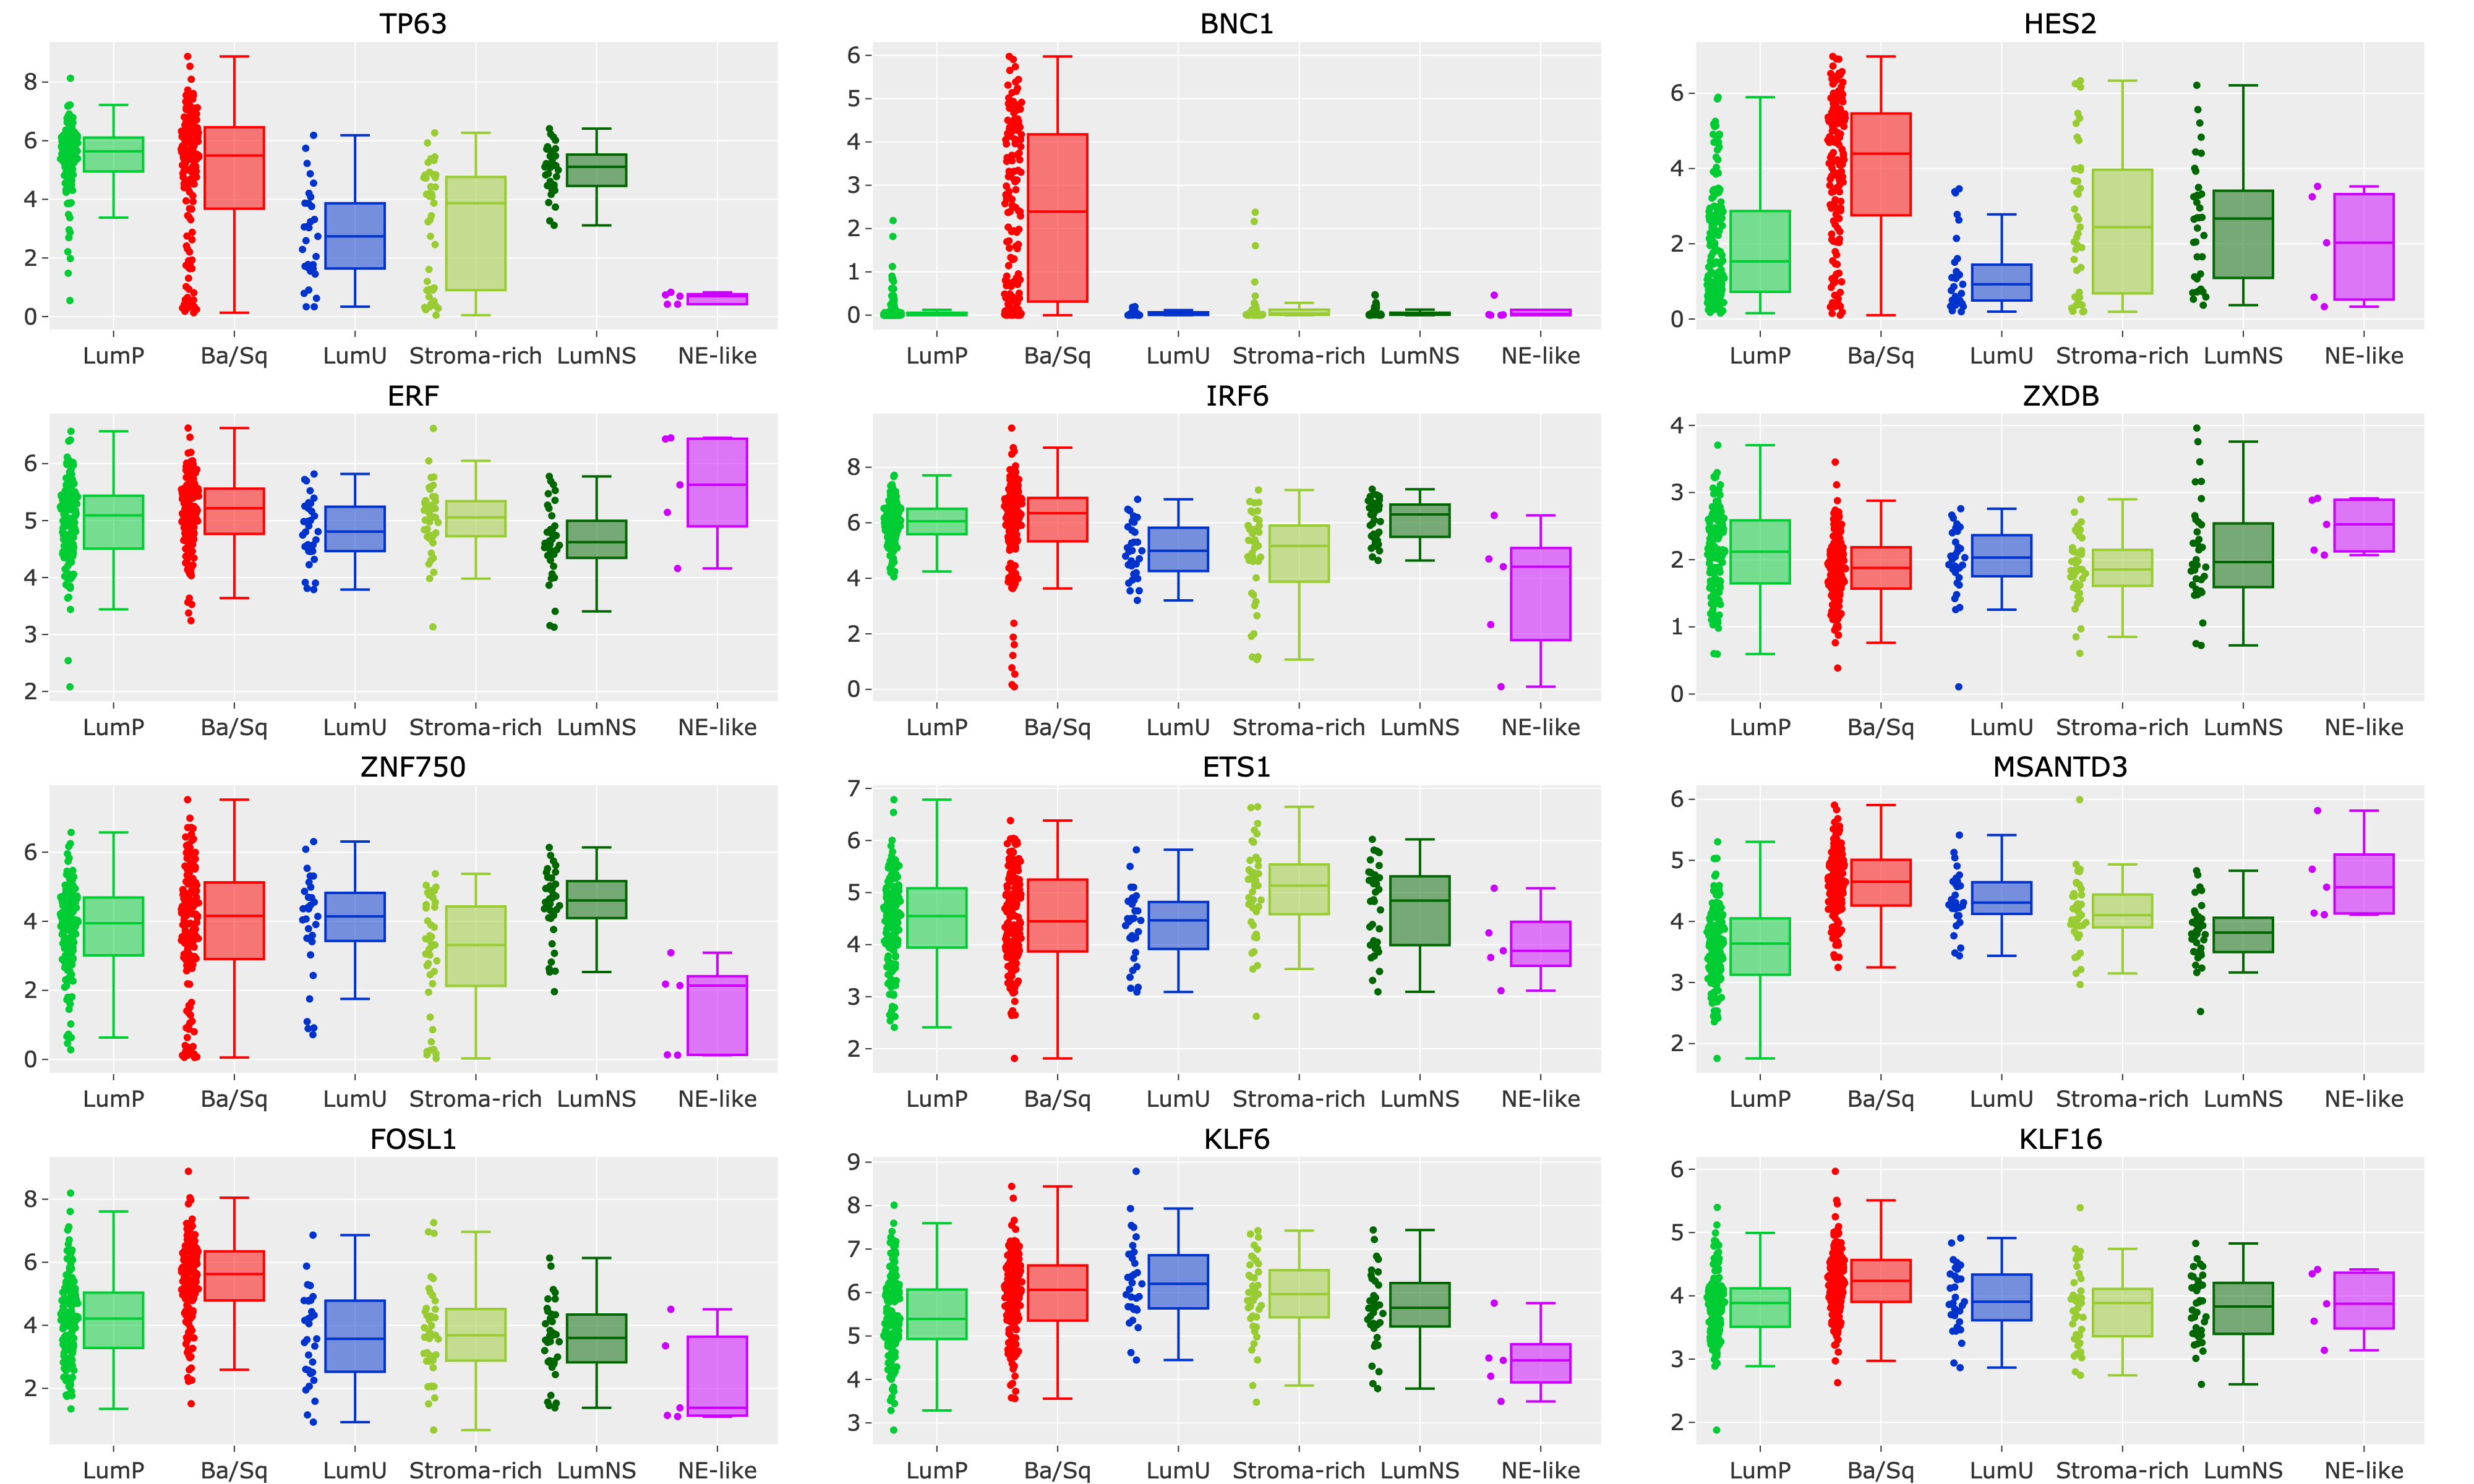
\includegraphics[width=1.0\textwidth,height=1.0\textheight,keepaspectratio]{Sections/Network_I/Resources/selective_pruning/log2_consensus_basal.png}
%       \caption{Consensus}
%       \label{fig:N_I:box_basal_consensus}
%   \end{subfigure}
%   % Dendrogram
%   \begin{subfigure}[!t]{1.0\textwidth}
%       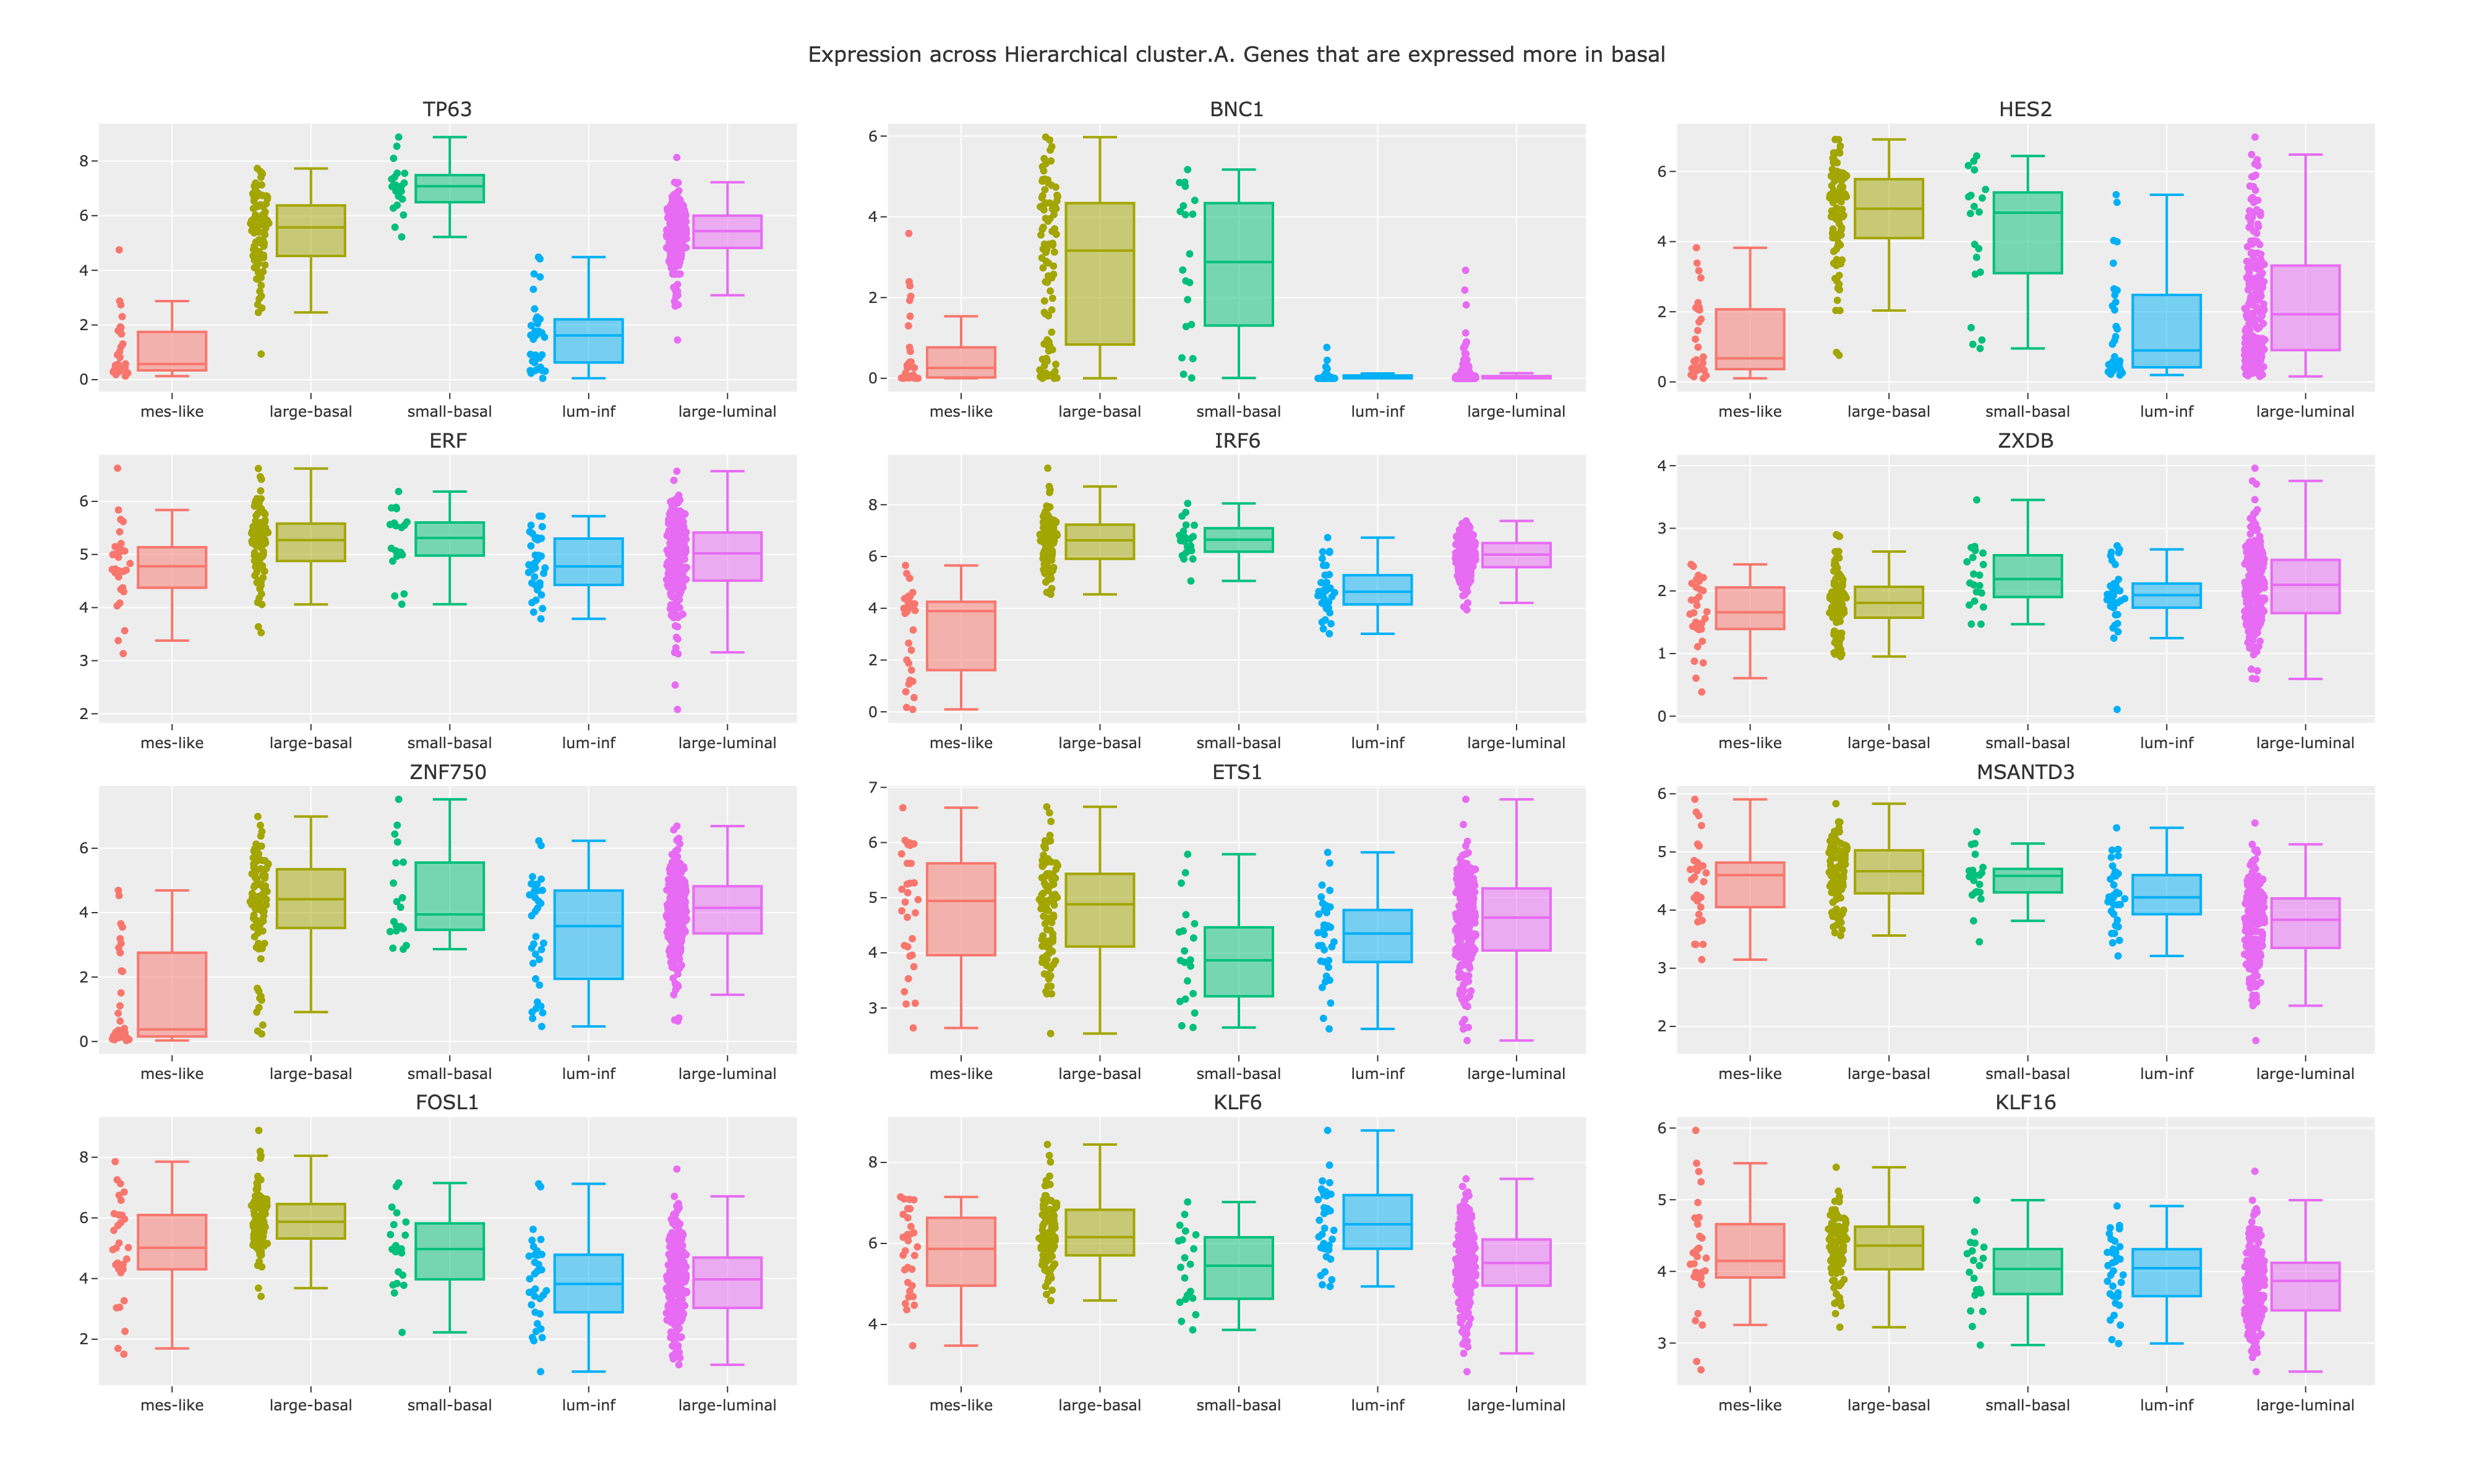
\includegraphics[width=1.0\textwidth,height=1.0\textheight,keepaspectratio]{Sections/Network_I/Resources/selective_pruning/log2_dendrogram_basla.png}
%       \caption{Basal}
%       \label{fig:N_I:box_basal_dendrogram}
%   \end{subfigure}
%   \caption{Box plots showing the $log2(TPM+1)$ of the \textbf{basal} markers over the consensus and groups derived from the hierarchical clustering applied in this chapter.}
%   \label{fig:N_I:box_basal}
% \end{sidewaysfigure}

% Luminal Markers
\begin{figure}[H]
    \captionsetup[subfigure]{justification=Centering}
  % consensus
  \begin{subfigure}[!t]{0.49\textwidth}
      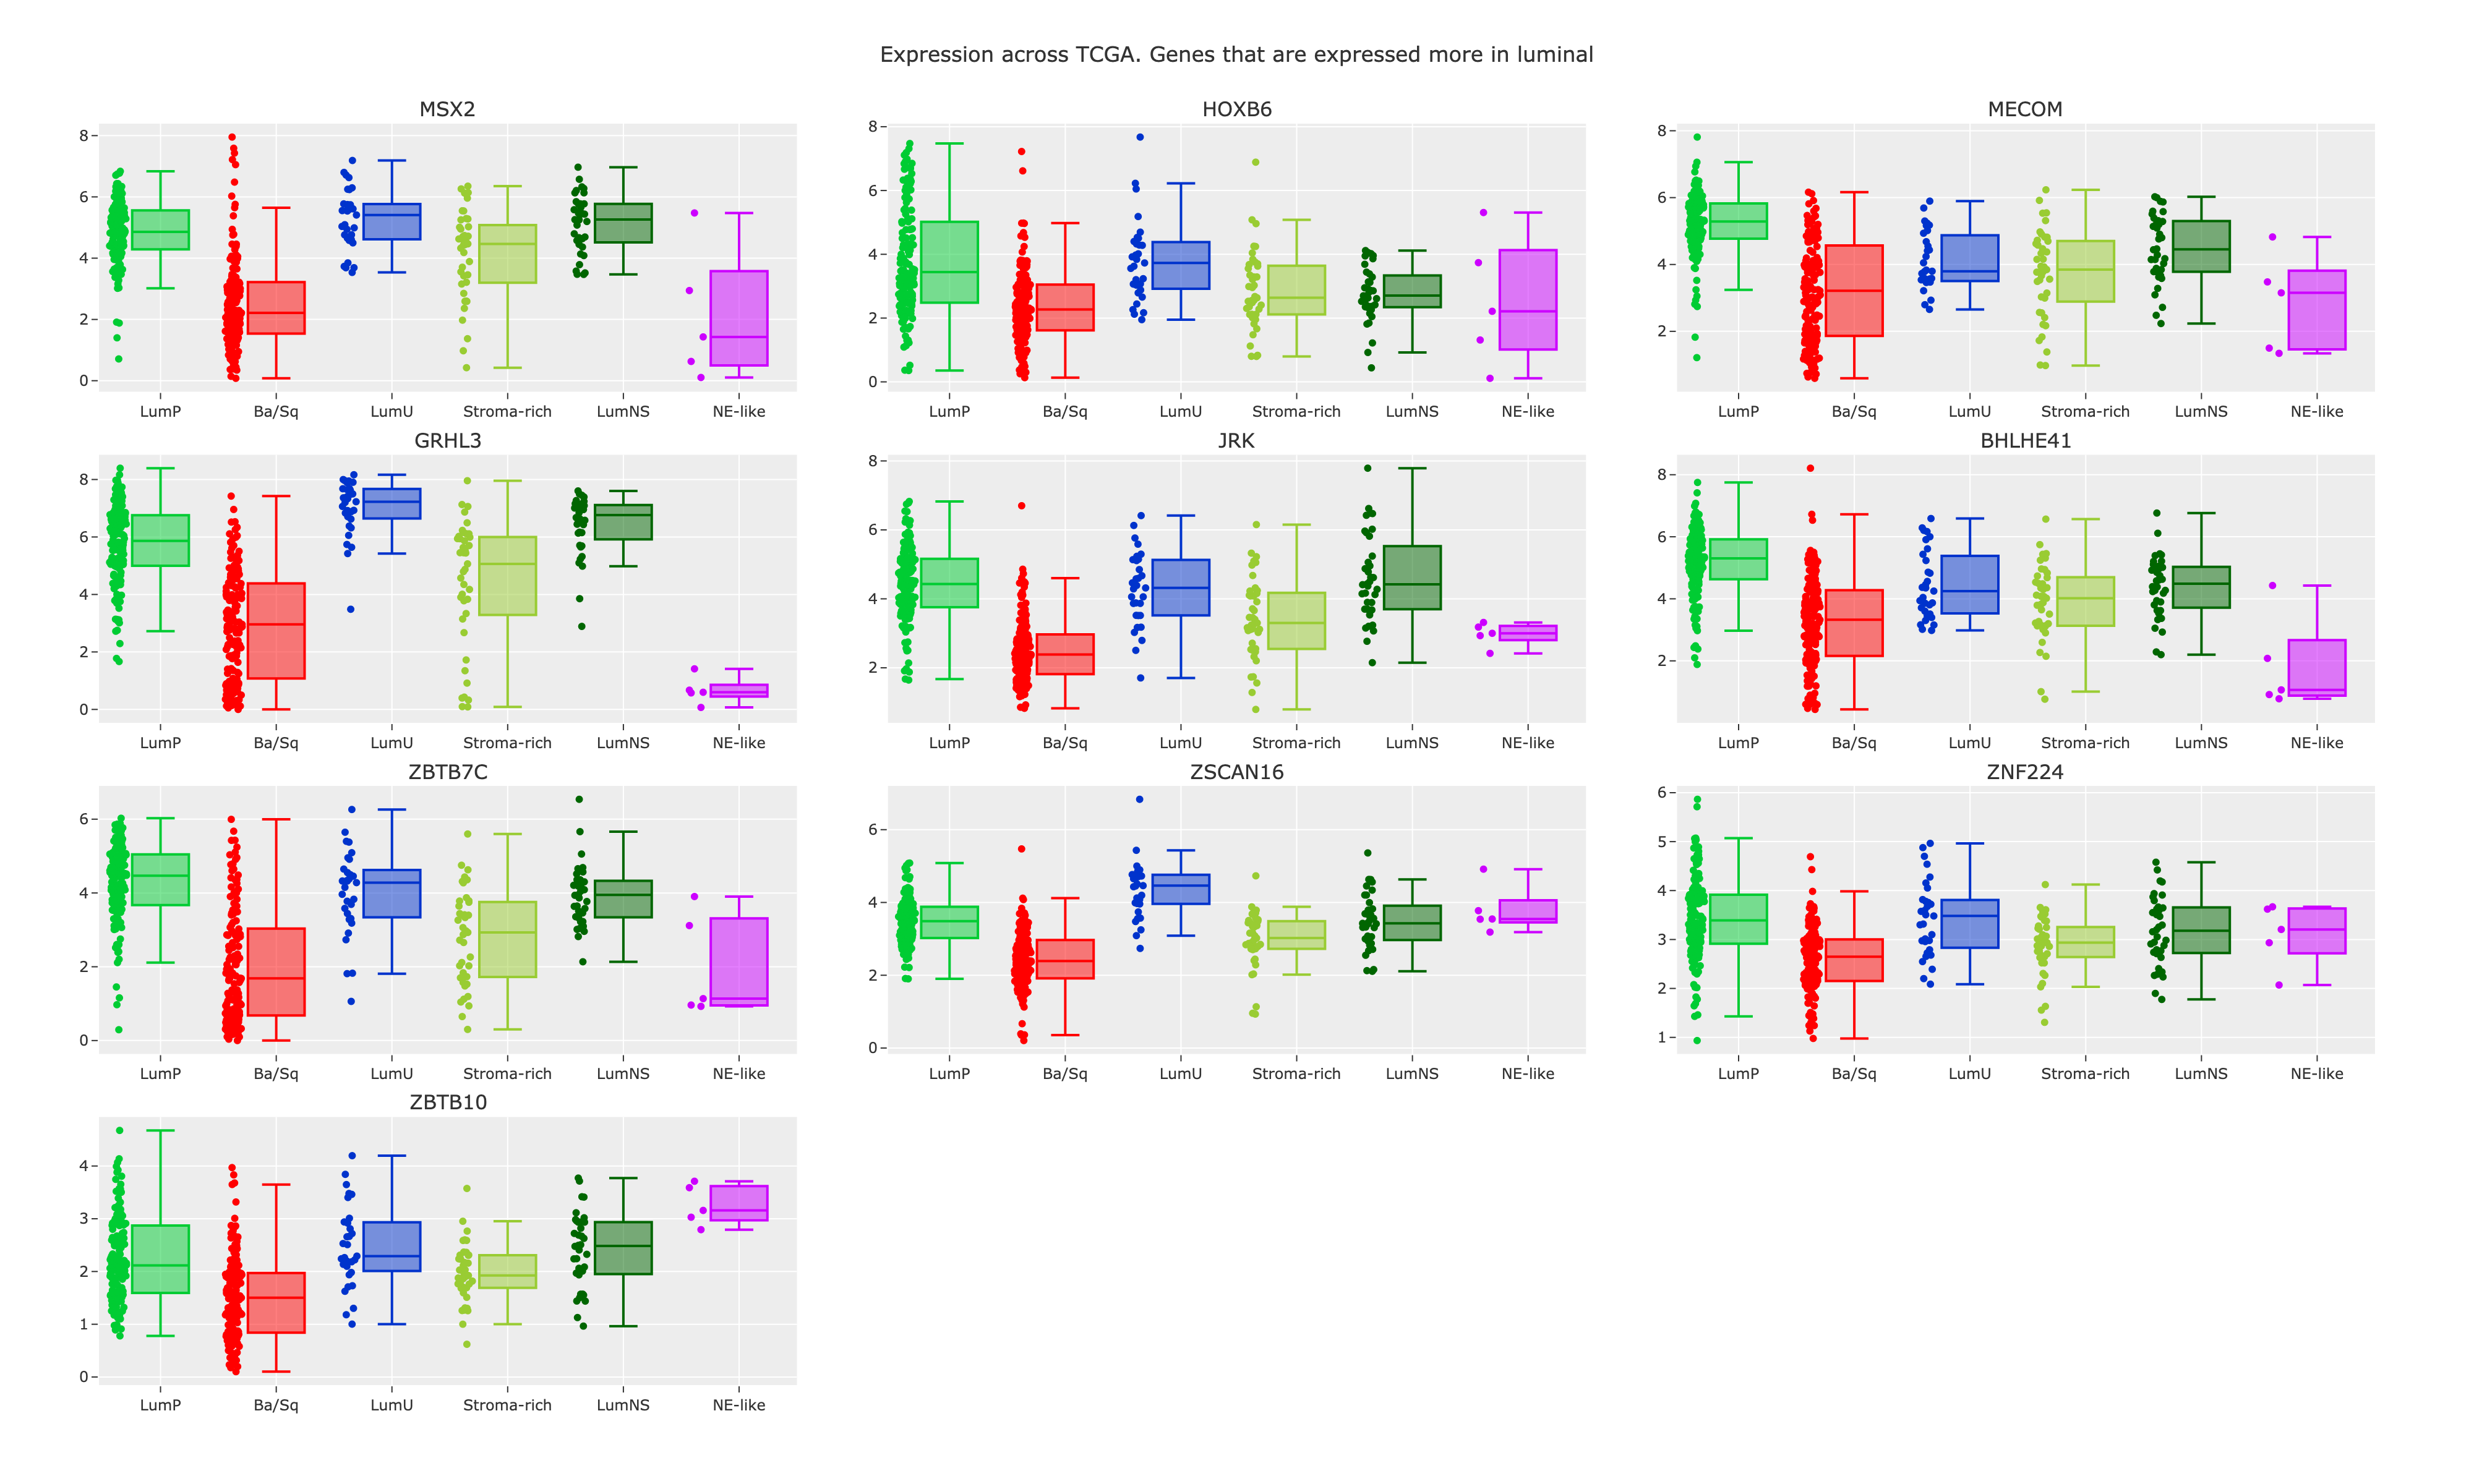
\includegraphics[width=1.0\textwidth,height=1.0\textheight,keepaspectratio]{Sections/Network_I/Resources/selective_pruning/log2_consensus_lum.png}
      \caption{Consensus}
      \label{fig:N_I:box_luminal_consensus}
  \end{subfigure}
  \begin{subfigure}[!t]{0.49\textwidth}
      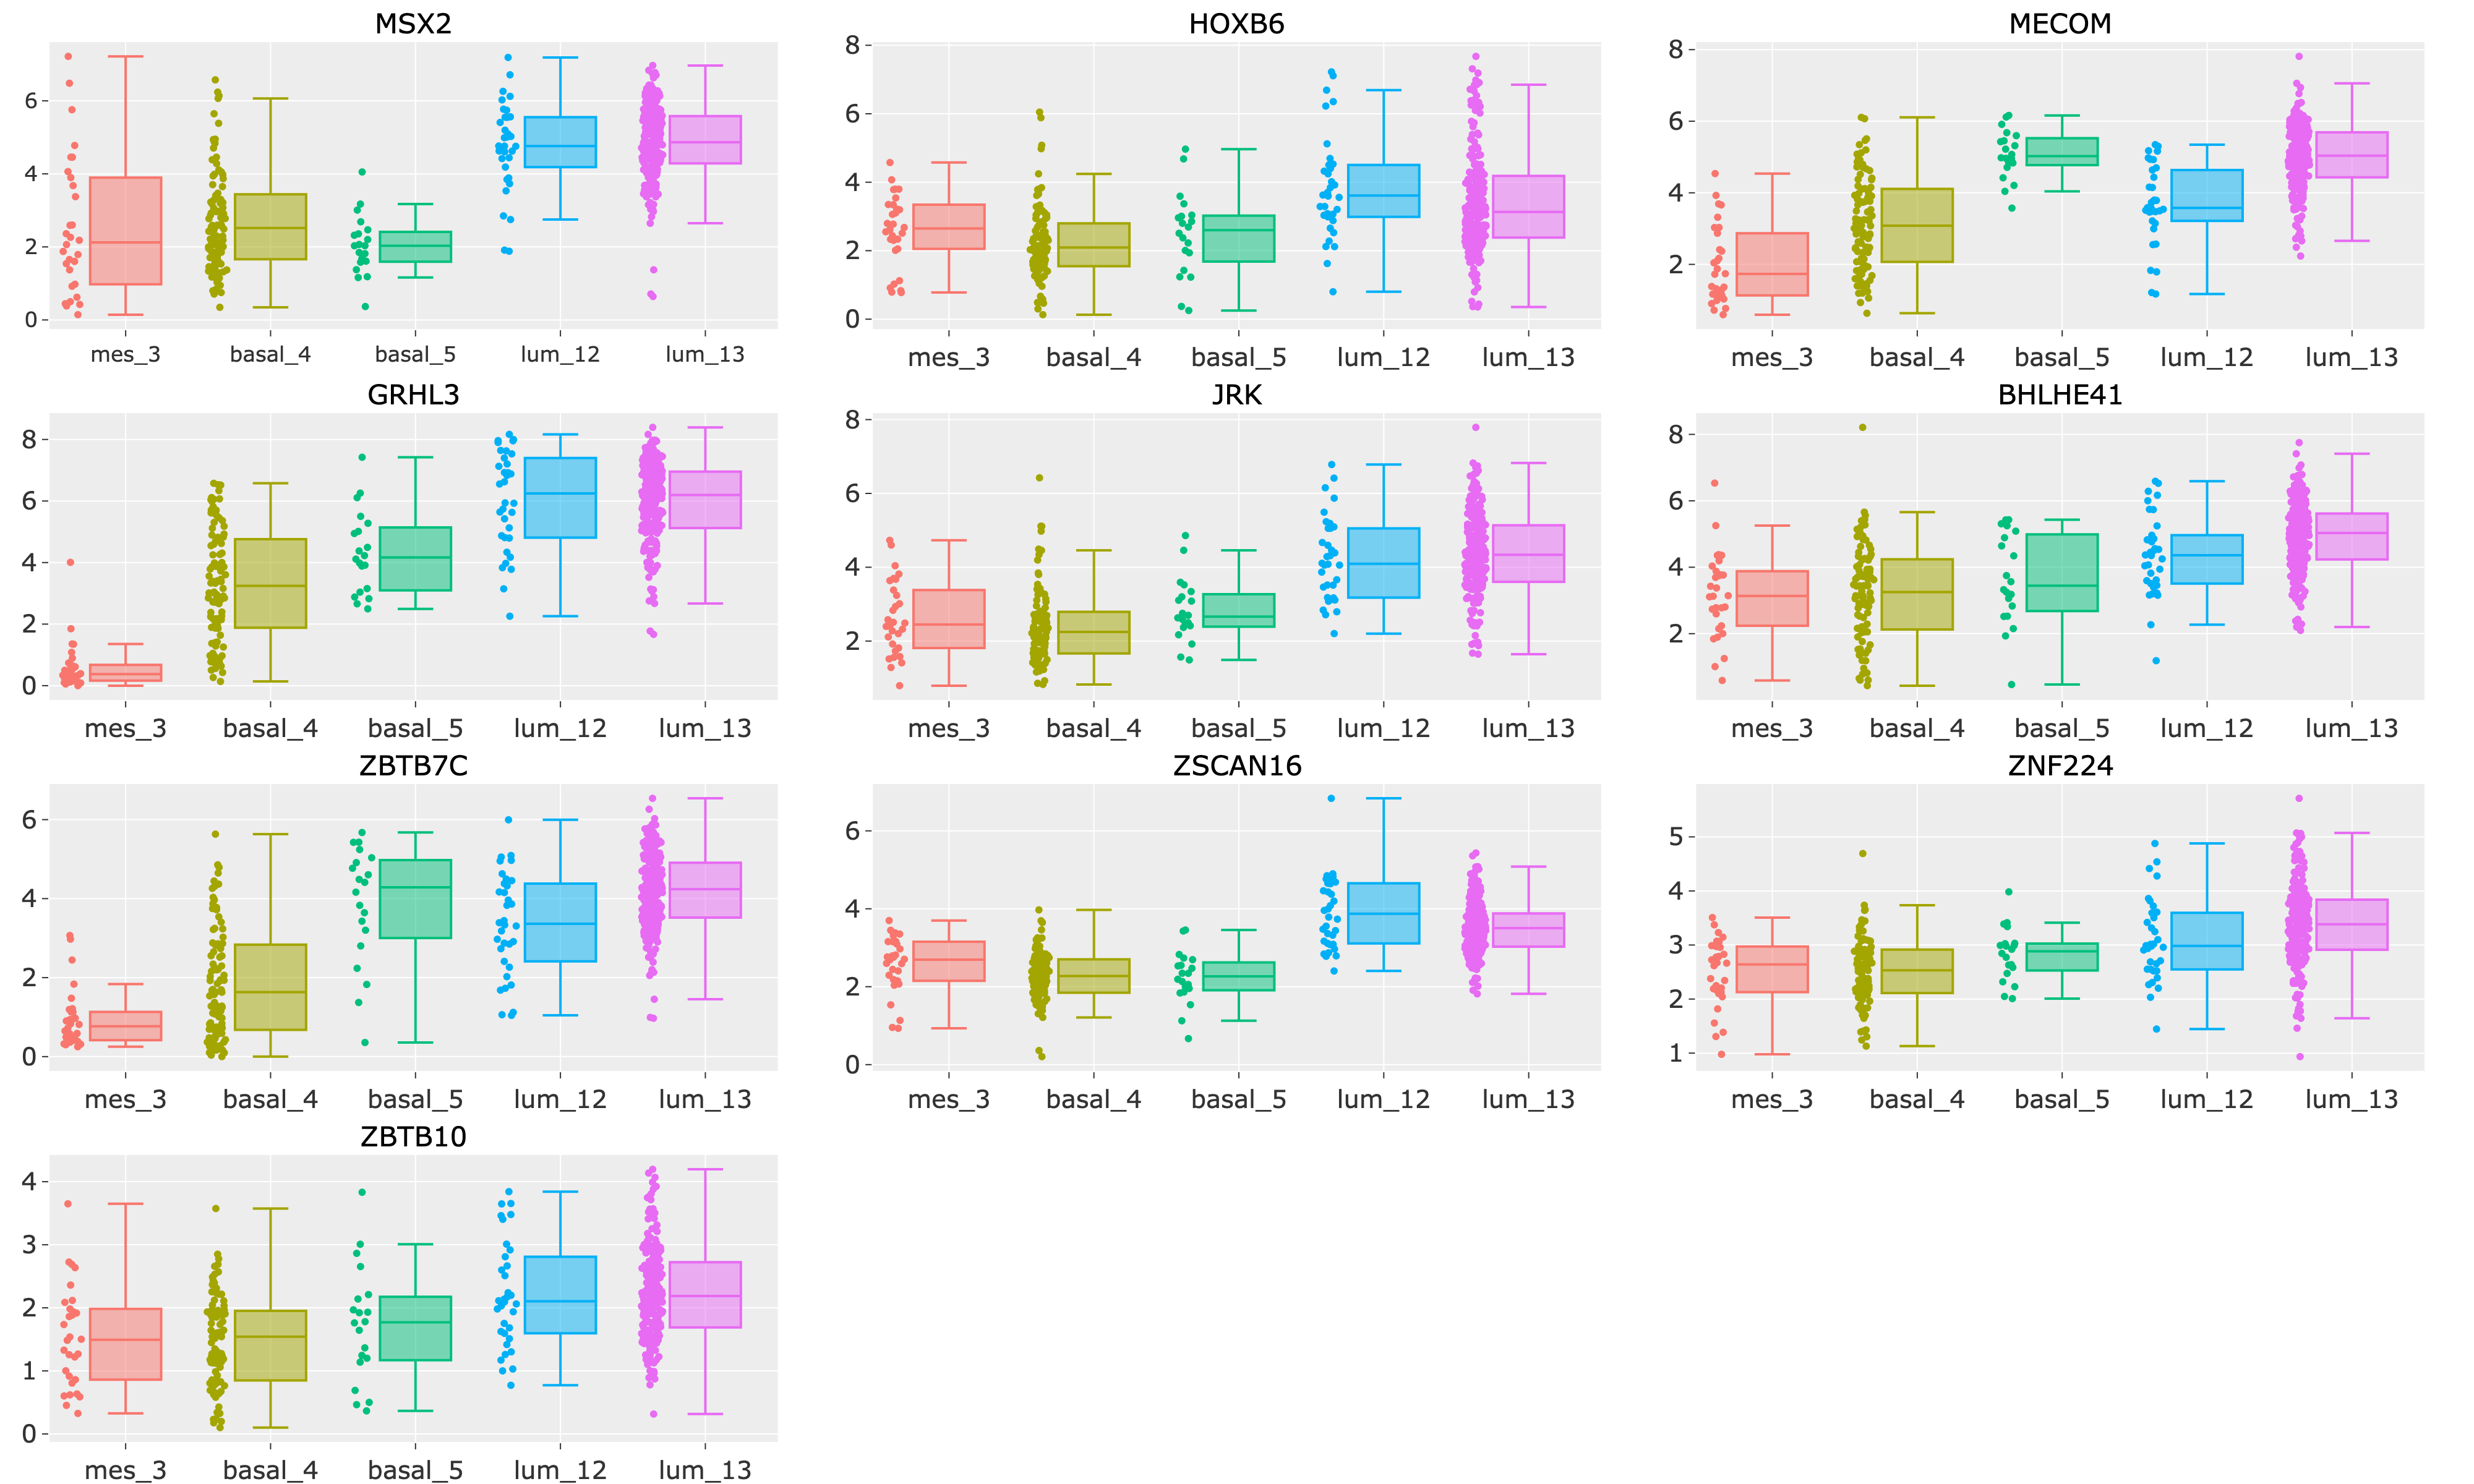
\includegraphics[width=1.0\textwidth,height=1.0\textheight,keepaspectratio]{Sections/Network_I/Resources/selective_pruning/log2_dendrogram_lum.png}
      \caption{Basal}
      \label{fig:N_I:box_luminal_dendrogram}
  \end{subfigure}
  \caption{Box plots showing the $log2(TPM+1)$ of the \textbf{luminal markers} over the consensus and groups derived from the hierarchical clustering applied in this chapter.}
  \label{fig:N_I:box_luminal}
\end{figure}


% Network stats
To leverage visualising aspect of the network, the basal/luminal markers were then searched in the experiment 5K genes network generated using no weight modifiers (standard), minimum 3 edges per genes and 6 for the TFs, and to which the Stochastic Block Model (SBM) was applied. Neither of the markers, basal/luminal or for differentiated, were not grouped in a single or 2-3 communities, but rather spread across several.

% Neighbours 
When filtering the network to display the neighbours of a  gene from the basal/luminal markers, it is often the case that markers are linked together, meaning that are co-expressed. \Cref{fig:N_I:net_MSX2} shows the sub-graph for \textit{MSX2} in which other markers such as \textit{FOXQ1, ZBTB7C} are linked directly to the gene. \textit{AHR} is also connected to \textit{MSX2}. \textit{AHR} has been extensively studies in the bladder cancer, urothelium and it is highly mutated in the TCGA cohort. It is also studied in more depth in the next chapter \ref{}. In the sub-network for \textit{BNC1} , \cref{fig:N_I:net_BNC1}, there are less known genes but \textit{CDH3} is a basal marker \citet{Dadhania2016-cb} and \textit{CAV1, CAV2}. 

It is worth noting that both genes, have considerable more than 6 neighbours. This suggests that there are many genes that have either \textit{BNC1} or \textit{MSX2} in their top correlated values. The kind of visualisation in \cref{fig:N_I:net_neighbours} is useful to narrow down the search for targets and potential co-expressed genes.

\begin{figure}[H]
    \captionsetup[subfigure]{justification=Centering}
\centering
\begin{subfigure}[!t]{0.49\textwidth}
    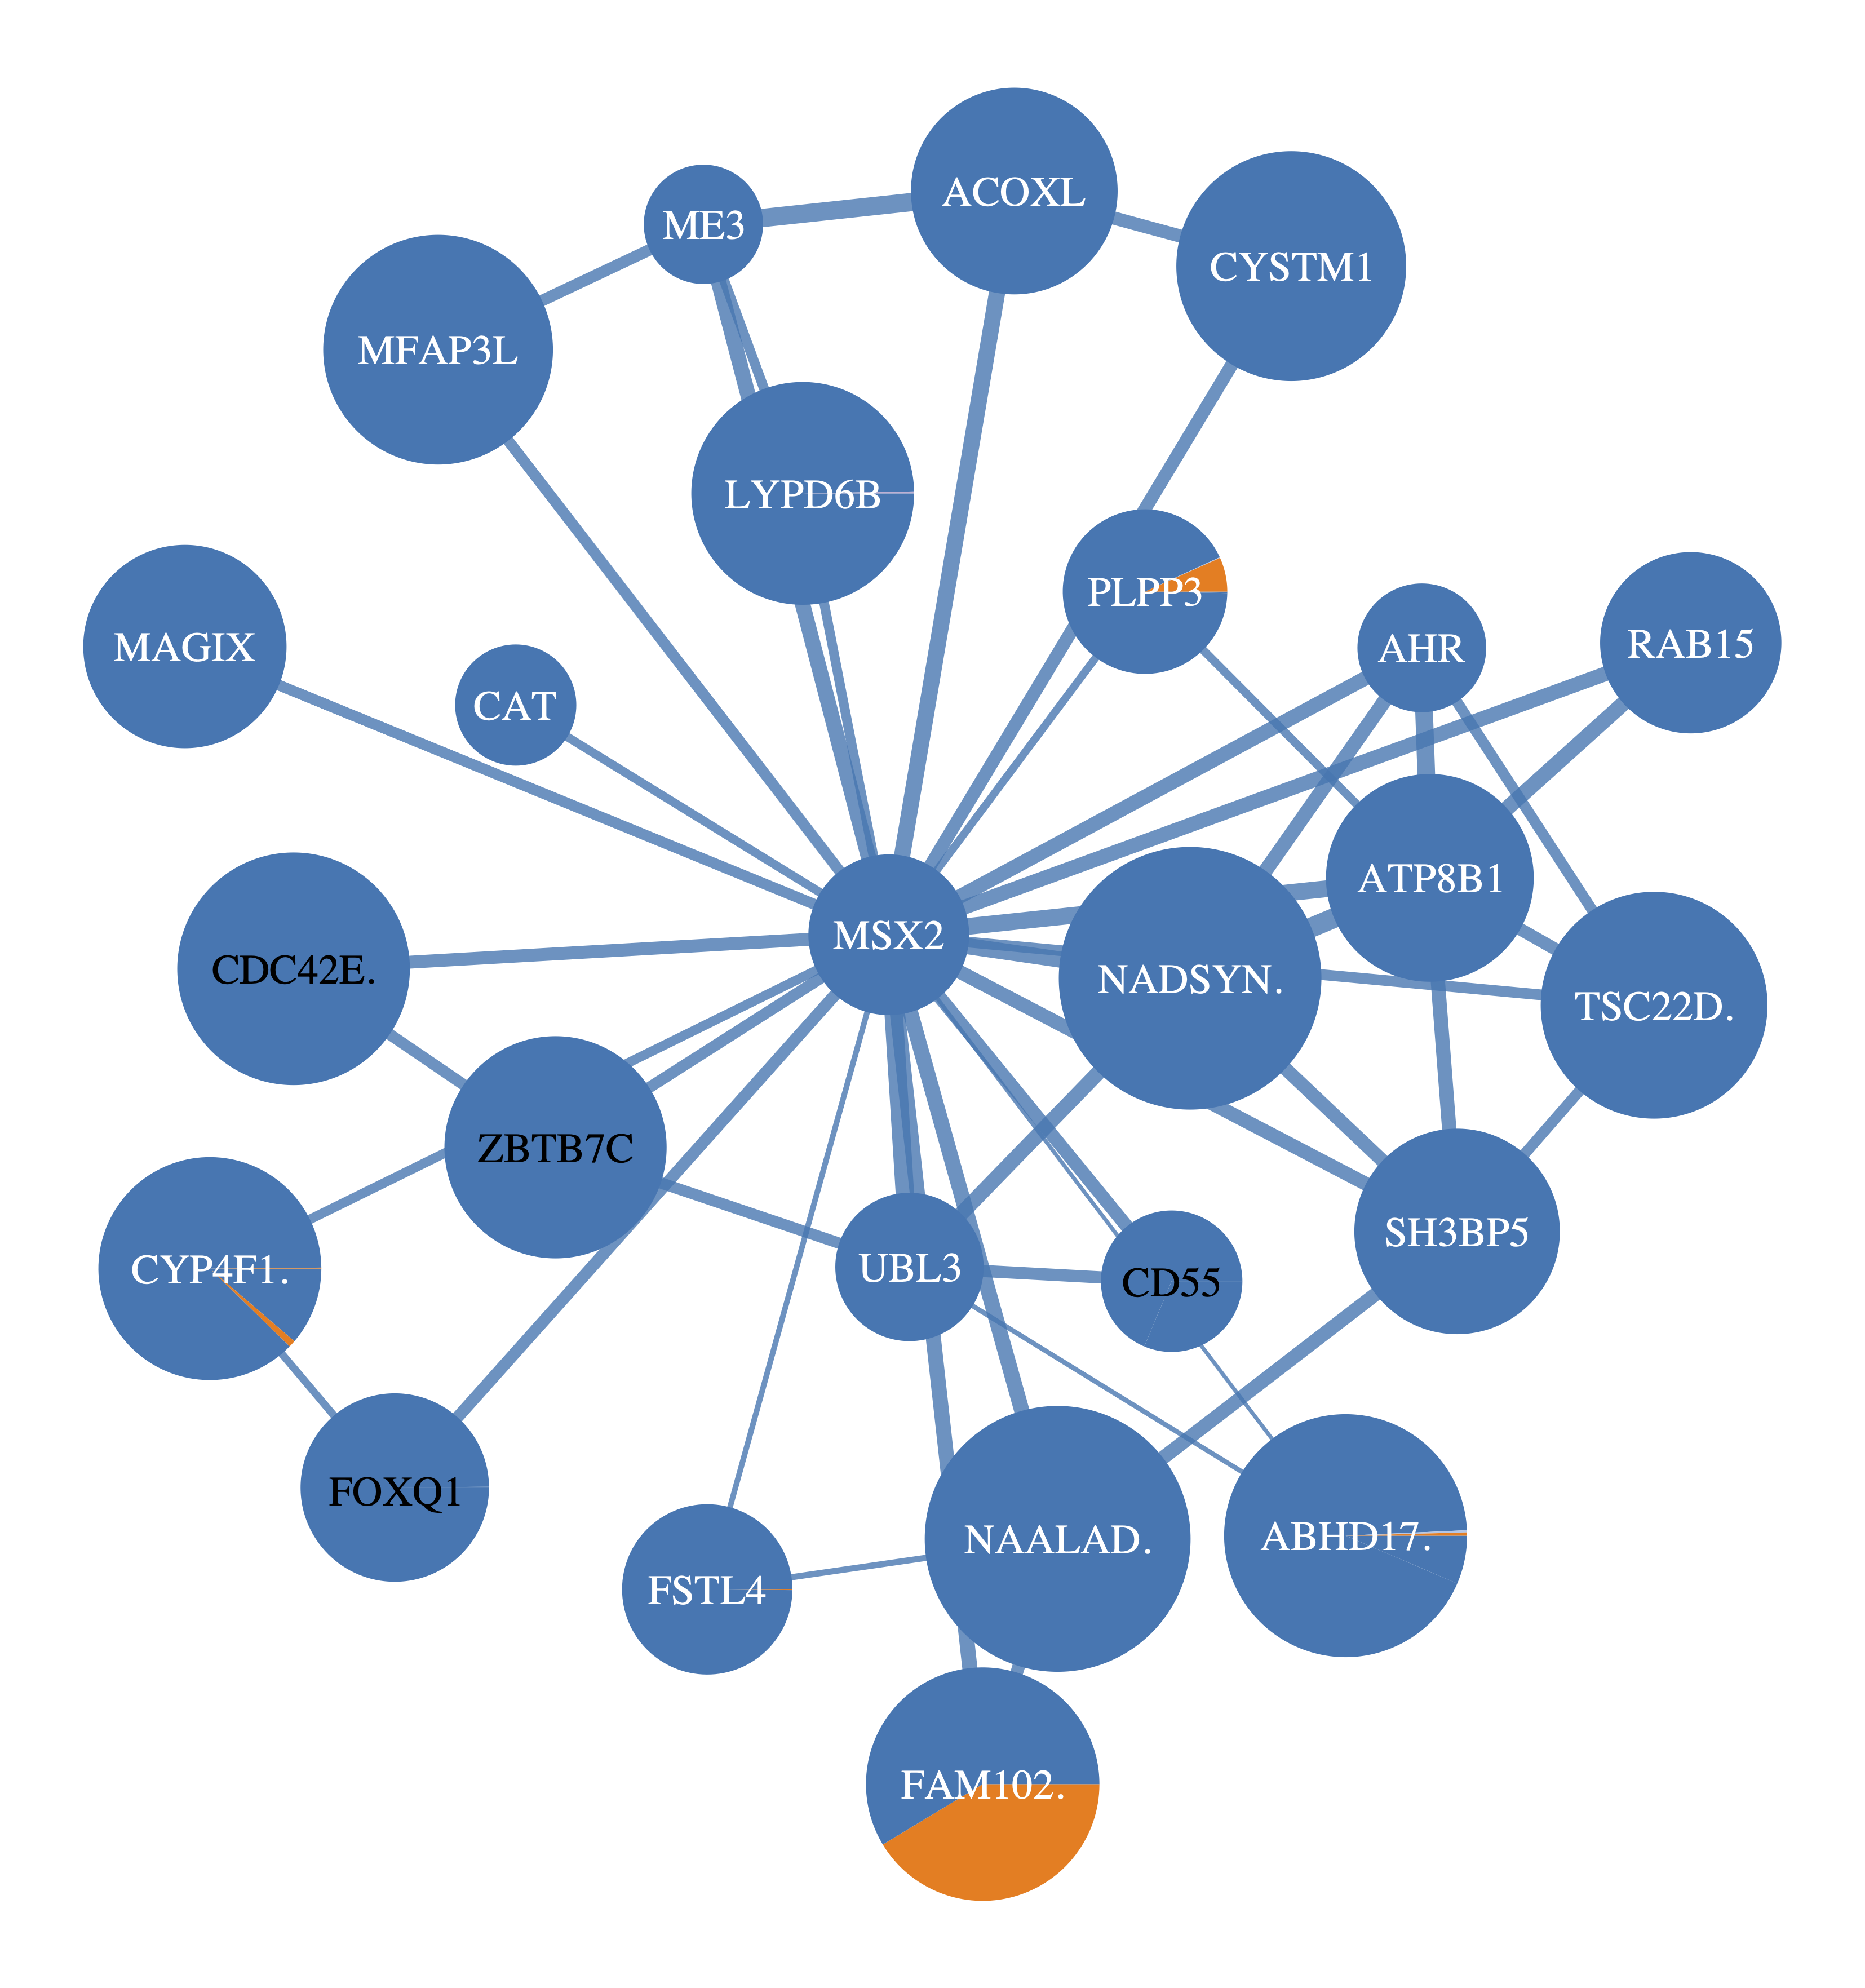
\includegraphics[width=1.0\textwidth,height=1.0\textheight,keepaspectratio]{Sections/Network_I/Resources/selective_pruning/net/net_MSX2.png}
    \caption{\textit{MSX2} (luminal)}
    
    \label{fig:N_I:net_MSX2}
\end{subfigure}
\centering
\begin{subfigure}[!t]{0.49\textwidth}
    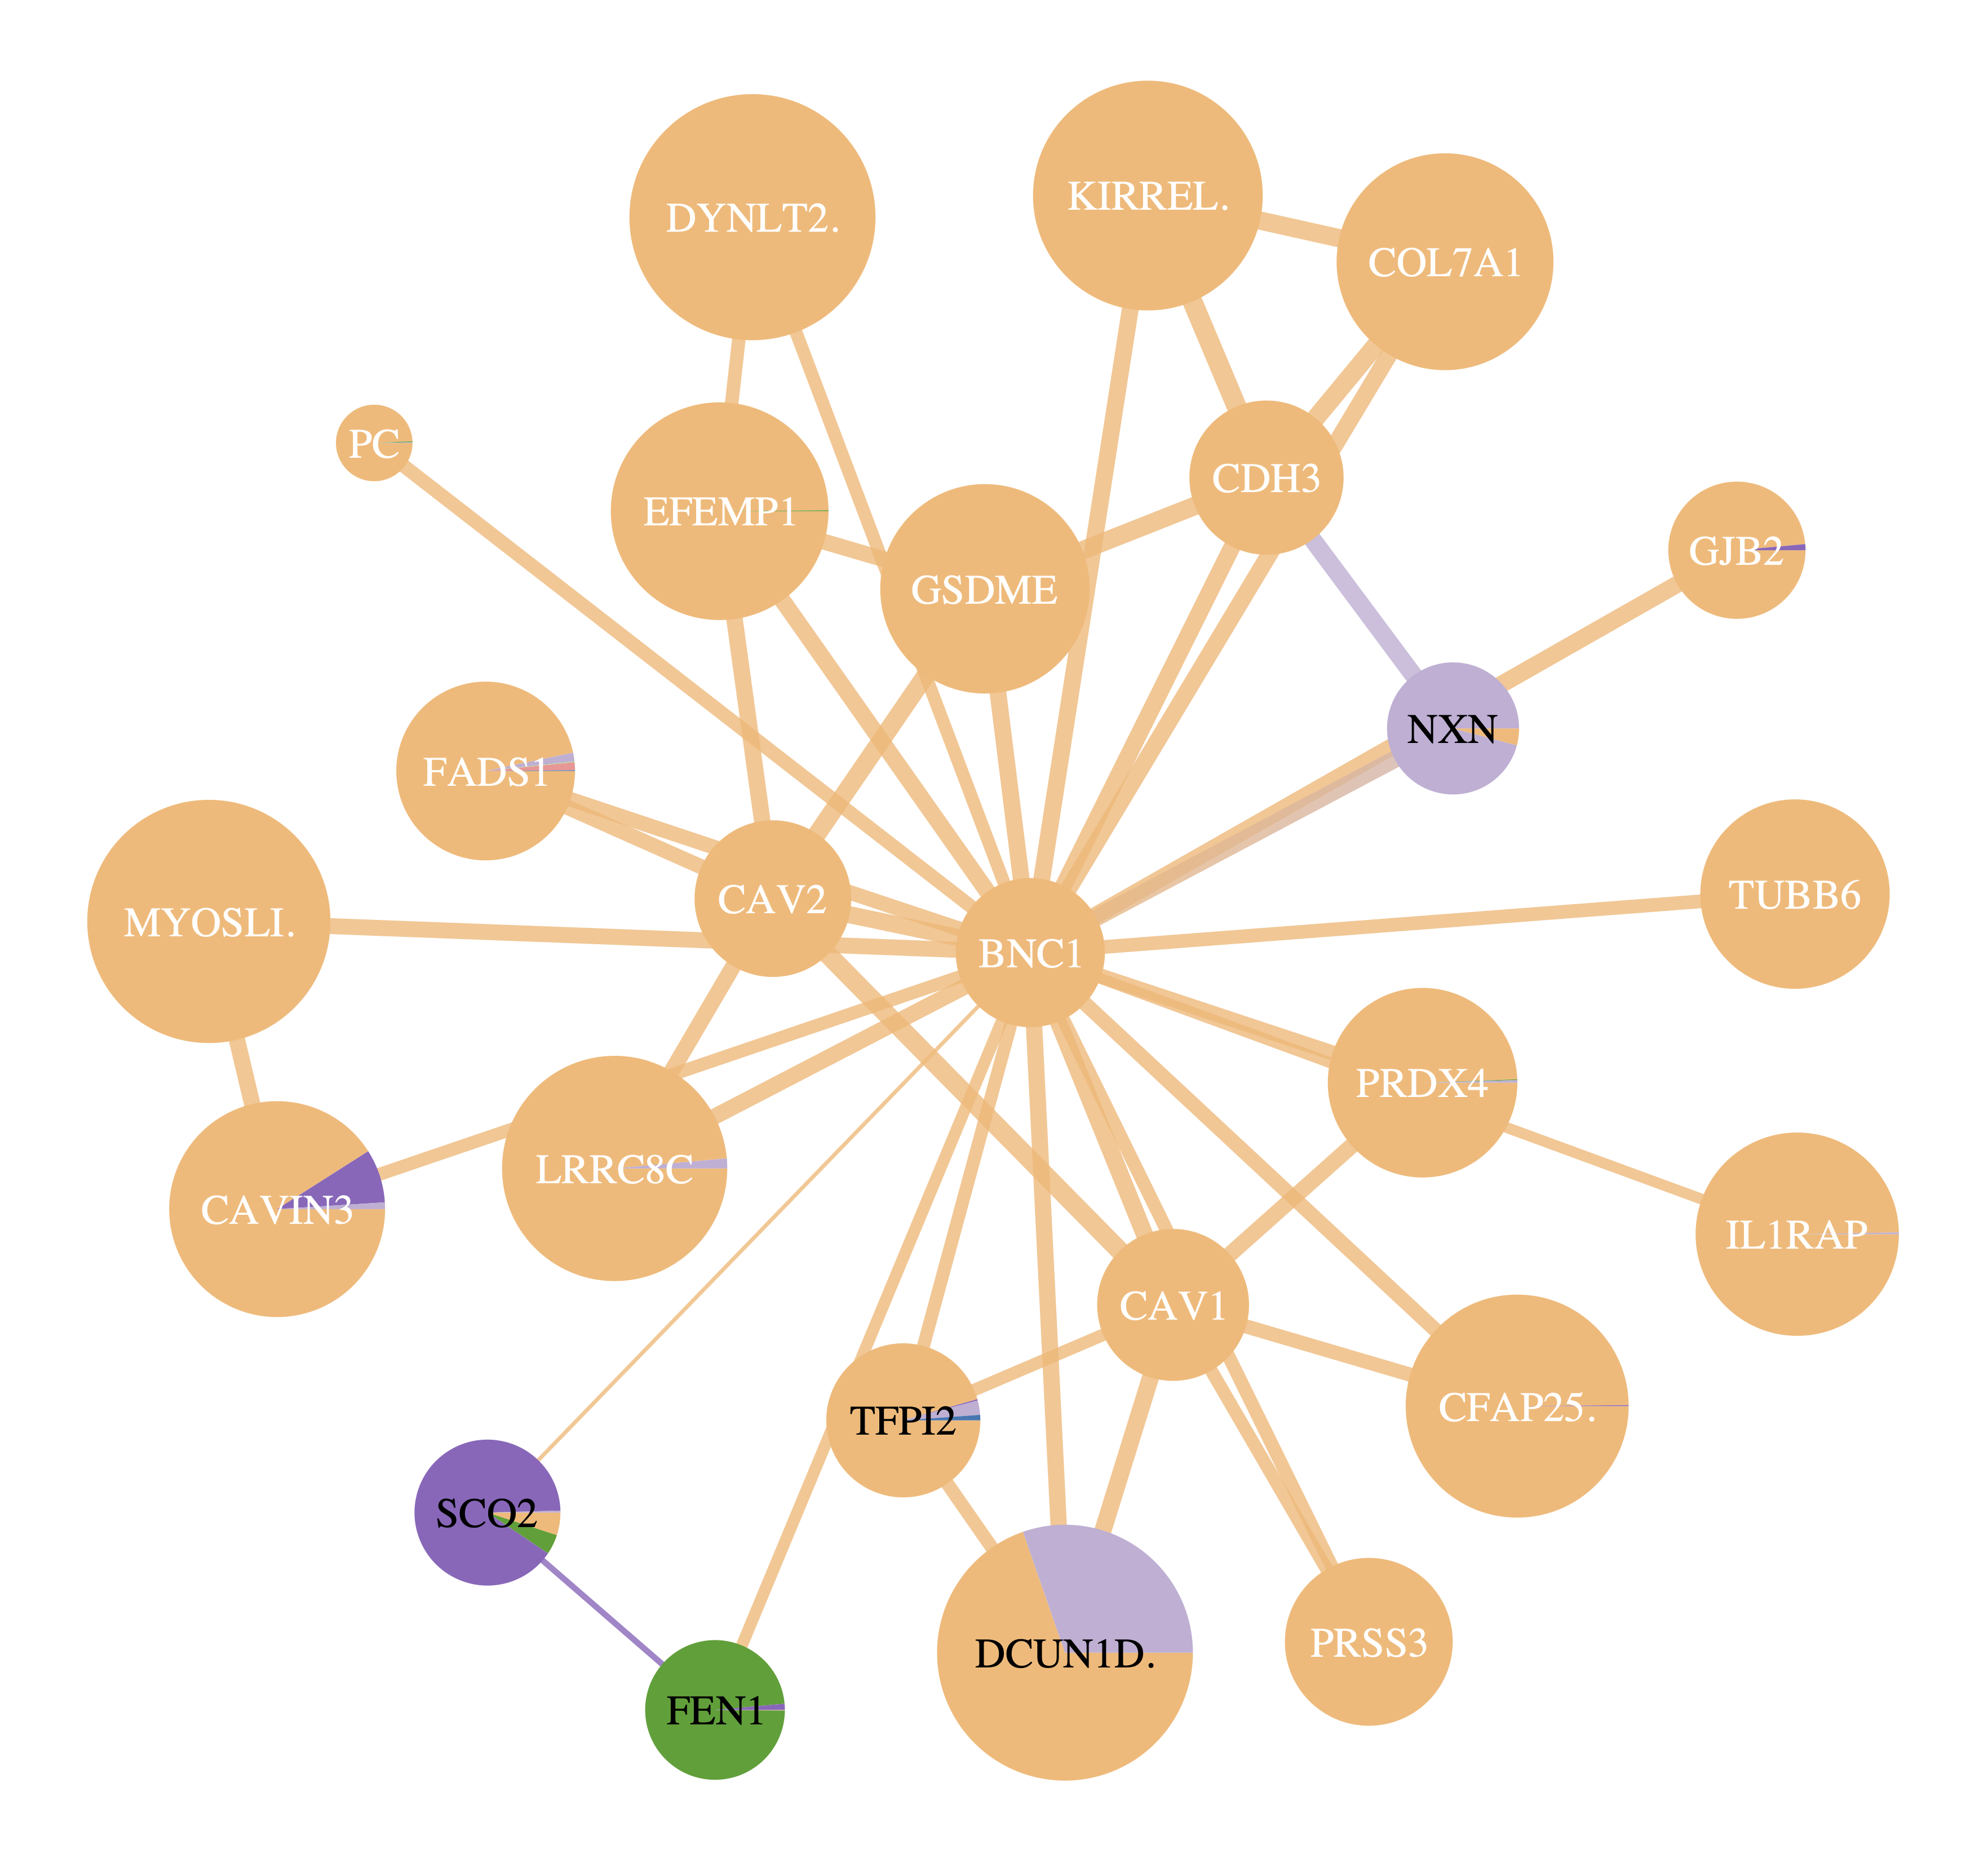
\includegraphics[width=1.0\textwidth,height=1.0\textheight,keepaspectratio]{Sections/Network_I/Resources/selective_pruning/net/net_BNC1.png}
    \caption{\textit{BNC1} (basal)}
    \label{fig:N_I:net_BNC1}
\end{subfigure}

    \caption{The \textit{MSX2} luminal and \textit{BNC1} markers and their neighbours in a standard network (no weight modifier), where a minimum of 6 edges are allowed per TF and the Stochastic Block Model was applied to detect the communities. The size of the nodes is proportional to the degree of the gene and the edge weight to the correlation value.}
    
    \label{fig:N_I:net_neighbours}
\end{figure}


Therefore, the 98 transcription factors and the two lists of Ba/Sq and Luminal markers are validated by research from different groups. The expression of these genes across the MIBC, from both the consensus and the subtypes derived from hierarchical clustering, can be seen in \cref{fig:N_I:box_basal,fig:N_I:box_luminal}. This also serves as an encouragement to explore the other genes not matched by other research, as they may exhibit potential for new biological insights.

% Subtypes analysis
\subsubsection*{Further exploring the derived subtypes} \label{s:N_I:sel_tfs_subtypes}

% Metadata exploration
To understand better the biology of the small basal group, the metadata from TCGA \citet{Robertson2017-mg} was used. Several metadata features were explored: level of smoking (cigarettes per day), race, metastasis, relation to noninvasive bladder cancer, and histology grade. \Cref{fig:ap:sel_tfs_tcga_metadata} from Appendix displays this information in the form of multiple histograms, where the x-axes represent the subtypes derived in this section and the y-axes the count of the metadata features. From the figure, there is no immediate characteristic for the small basal group, neither with the Squamous pathology nor with the metastatic status, but most of the patients were smokers. It is worth pointing out that LumInf, Mes-like, and large luminal groups are generally characterised by non-squamous tumours. From Appendix \Cref{fig:ap:sel_tfs_tcga_meta_mut} shows that there is no immediate relationship with the mutations selected in the TCGA supplementary material, while \cref{fig:ap:sel_tfs_tcga_meta_apobec} (appendix) shows no relationship with the \textit{APOBEC} mutation.

% Pi plot for Small Ba/Sq
\begin{figure}[!htb]   
\centering
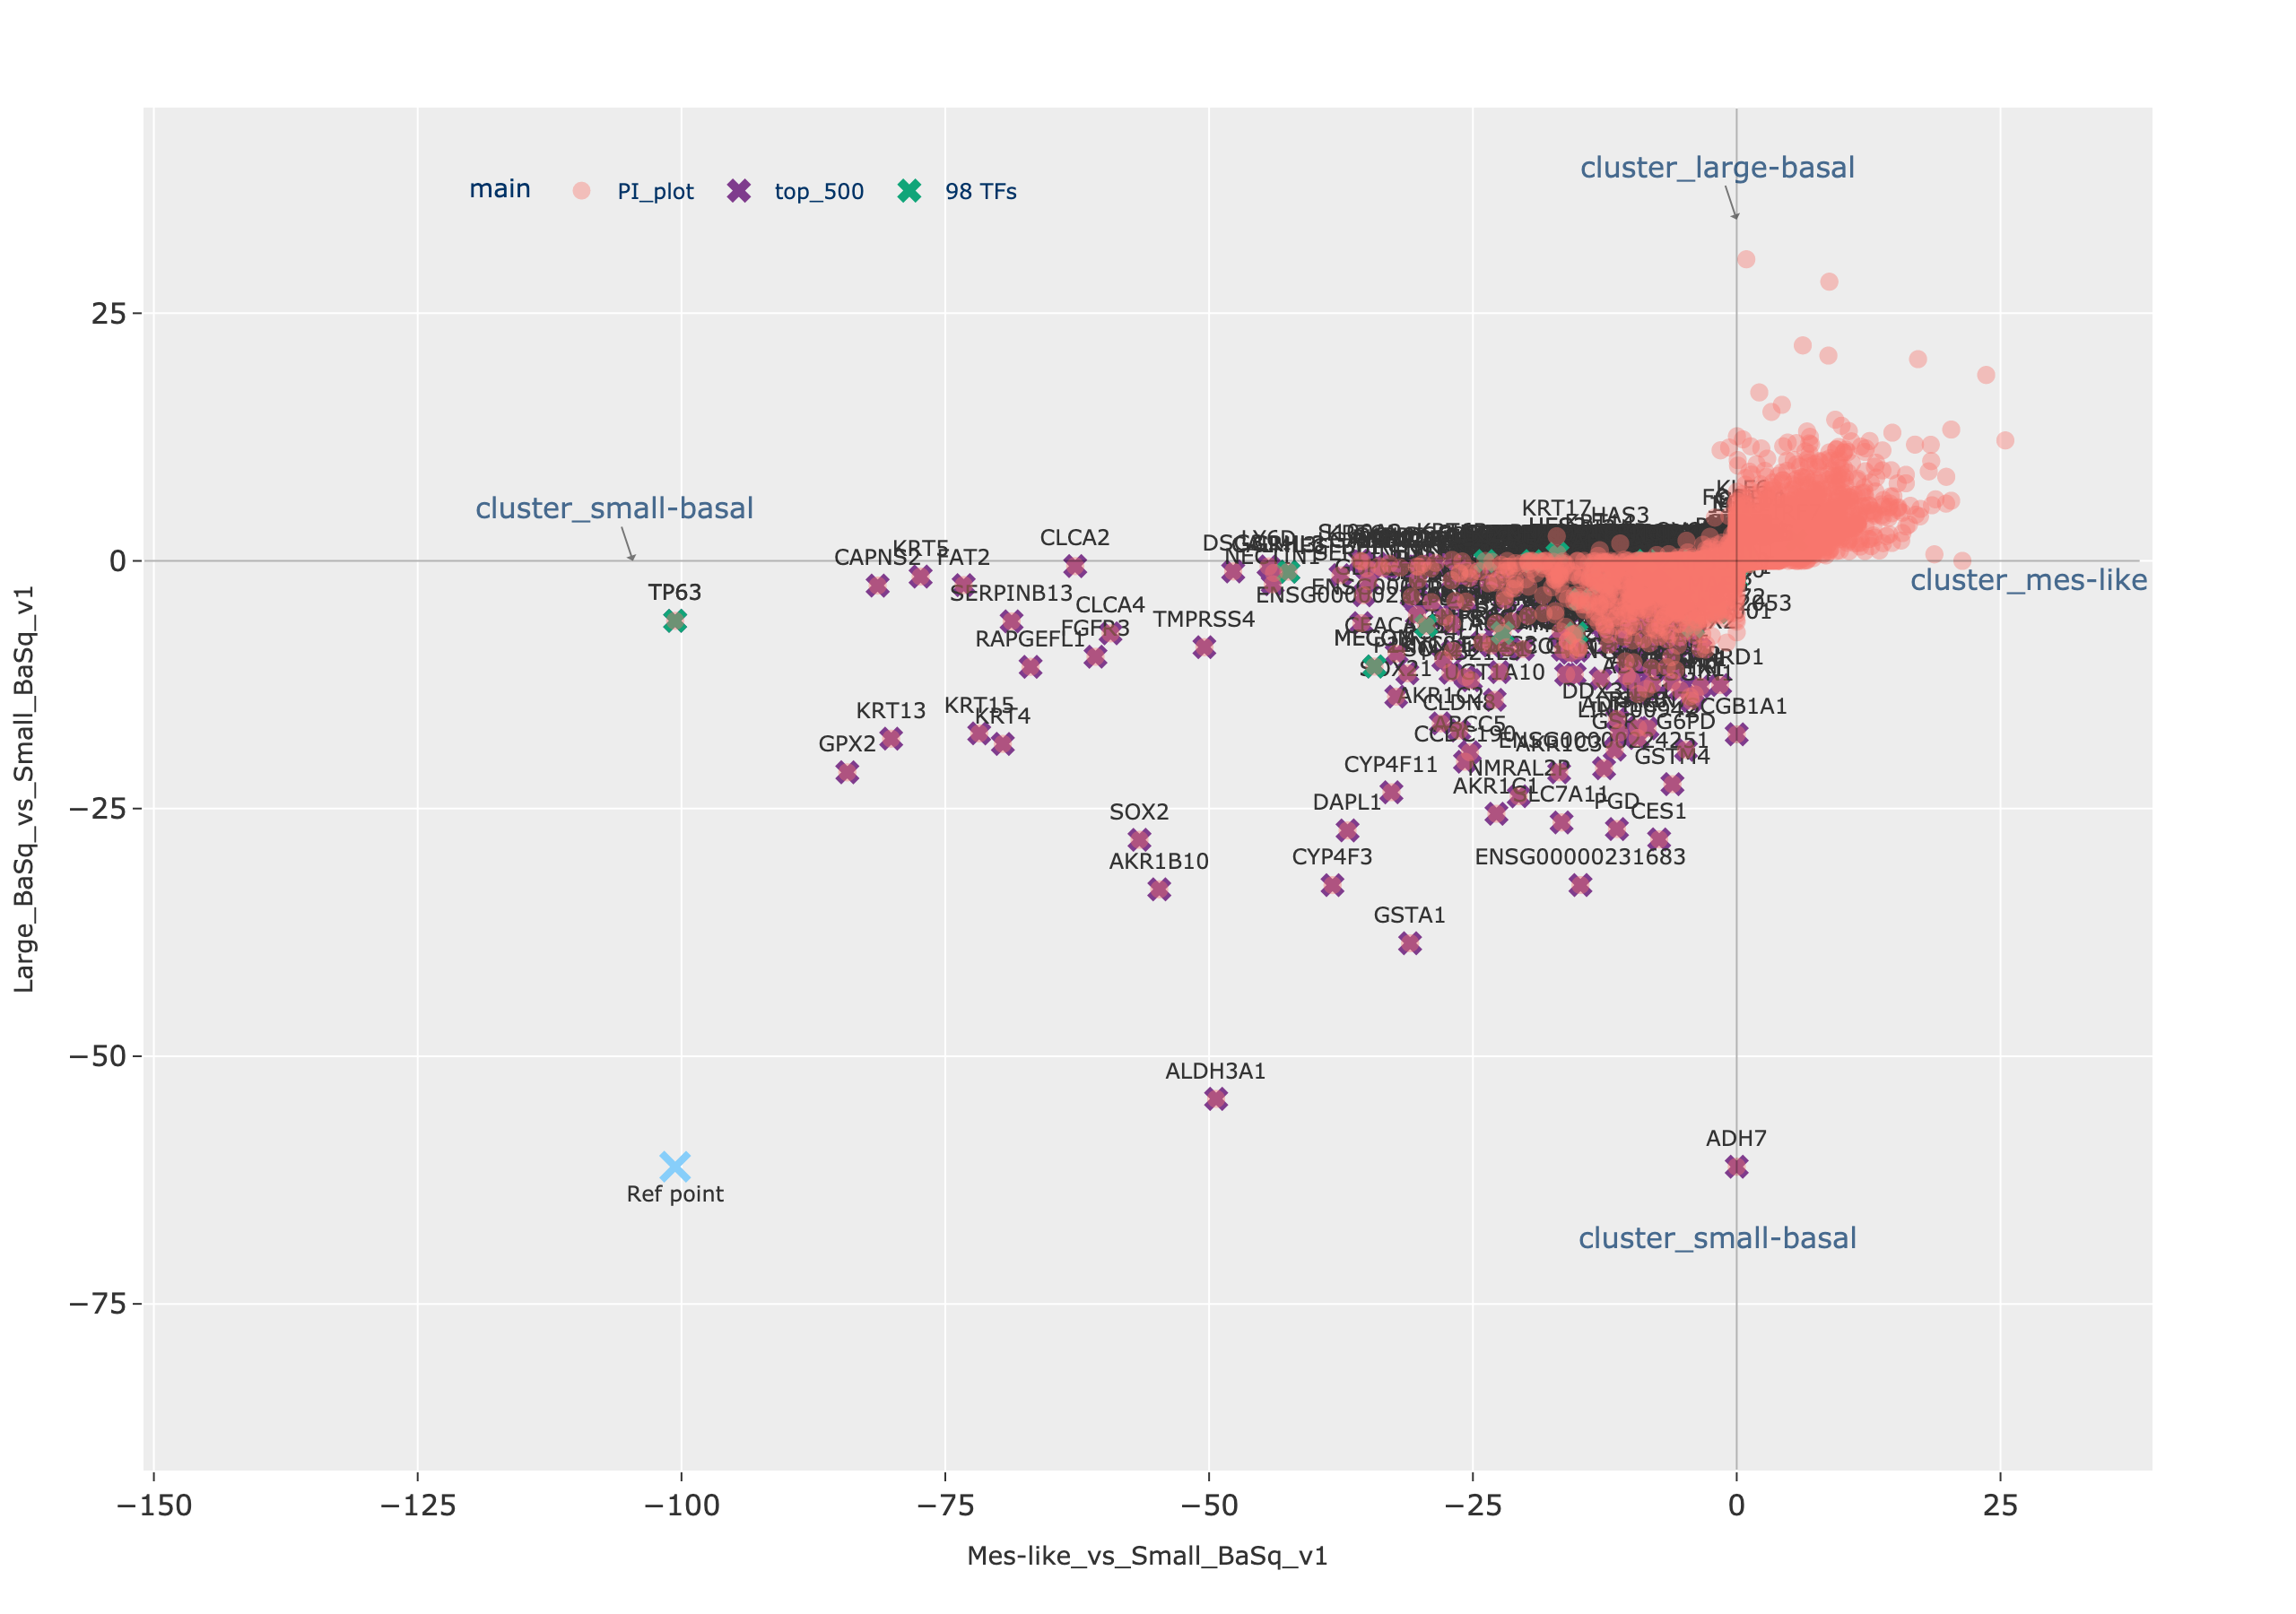
\includegraphics[width=1.0\textwidth,height=1.0\textheight,keepaspectratio]{Sections/Network_I/Resources/selective_pruning/pi_gsea/pi_smallBasal.png}
  \caption{Pi plot showing the Small Basal vs Large Basal on the X-axis, and Small-Basal vs Mes-like Y-axis. This plot highlights the genes that are high and significantly expressed in the Small Basal subtype. }
\label{fig:N_I:pi_smallBasal_comp}
\end{figure}

% pi plot
Differentially expressed analysis (DEA) was performed between the MIBC groups derived from the gene expression of the 98 TFs. The analysis enables to compare cancer subtypes beyond the transcription factors, and to find the genes that are significantly expressed to each subtype. For every MIBC group, a pi scatter plot is used as in \cref{fig:N_I:pi_smallBasal_comp}, where there is a quadrant (here - III) that holds the genes specific to that subtype with respect with the compared groups. In \cref{fig:N_I:pi_smallBasal_comp} the small basal (5 from \cref{fig:N_I:sel_tfs_cs_analysis}) is compared against the large basal, on the x-axis, in order to determine the properties over the other basal. The pi-values on the y-axis are the result from small-basal vs mes-like as it was observed that the mes-like group is different from both the luminal\footnote{The purpose of the pi plot was to highlight the specific genes to the small-basal. However, one may think that a more direct comparison of the small-basal with the luminal groups could have been chosen, instead of mes-like DEA. The other pi-plots comparison (like the plots for LumInf,  large luminal \cref{fig:ap:pi_other_values_I,fig:ap:pi_other_values_II} - in Appendix) cover the 'basal' vs 'luminal' comparison. }. The light-blue marker in quadrant III represents the referential point to which the genes are 'the most' enriched in the small-basal, and the closest 500 genes to the referential point are coloured in purple. 


% Introduce the GSEA
The distance to the referential marker is computed for each point in the scatter plot \cref{fig:N_I:pi_smallBasal_comp} and then ranked in descending order. This means that all the points in the pi-plot are ranked by how much these are differentially and significantly are expressed in the small basal group. It also allows to run the pre-rank method for Gene Set Enrichment Analysis (GSEA) using the \textit{GSEAPY} library \citet{Fang2023-ec}. The pre-rank GSEA was configured to 1000 permutations (lowering the chance of misidentifying pathways) and the False Discovery Rate (FDR) of the q-value was kept at 0.05. The same process was repeated for the other subtypes based on their corresponding pi-plots\footnote{The pi-plot figures were also used to verify the results from GSEA. The genes found in the top pathways were plotted back on the plot to check if these are in the quadrant specific to the subtype studied.}; see \cref{s:ap:sel_prun_pi}.

% Why the top terms are kept
Taking a step back, the input data for GSEA for each subtype is taking the same (large) list of genes but it is ranked differently, giving more importance to the genes specific to the studied subtypes. The GSEA results will then shared a large number of found pathways at each run. To address this, the ten terms with the highest normalised enrichment score (NES) were kept for each MIBC subtype GSEA run. Having a restricted subset of term allows to find the exclusive pathways for a subgroup. Reactome 2023 v2 was used as the database to search for pathways in this section as it contains the up-to-date canonical pathways, it is medium size (1692 gene sets) as well the names are easier to interpret The output from the GSEA can be seeen in which can be seen in the tables \cref{tab:N_I:gsea_basal_reactome,tab:N_I:gsea_luminal_reactome}.

% GSEA basal table (reactome)
\begin{table}[H]
  \centering
  \scriptsize
  \begin{tabularx}{\textwidth}{>{\hsize=1.7\hsize}X|>{\hsize=0.4\hsize}X|>{\hsize=0.4\hsize}X|>{\hsize=0.6\hsize}X|>{\hsize=0.4\hsize}X|>{\hsize=0.15\hsize}X}
    \toprule
    \textbf{Term} & \textbf{NES} & \textbf{FDR q-val} & \textbf{\# lead} & \textbf{\# matched} & \textbf{ratio} \\
    \midrule
    \multicolumn{6}{c}{\textbf{smallBasal}} \\
    \midrule
    NFE2L2 REGULATING ANTI OXIDANT DETOXIFICATION ENZYMES & 2.486 & 0 & 13 & 13 & 1 \\
    \midrule
    RND1 GTPASE CYCLE & 2.158 & 0 & 31 & 23 & 0.742 \\
    \midrule
    REGULATION OF RUNX1 EXPRESSION AND ACTIVITY & 2.114 & 0 & 11 & 8 & 0.727 \\
    \midrule
    SIGNALING BY PDGFR IN DISEASE & 2.101 & 0 & 13 & 9 & 0.692 \\
    \midrule
    RORA ACTIVATES GENE EXPRESSION & 2.082 & 0 & 15 & 13 & 0.867 \\
    \midrule
    GLUTATHIONE CONJUGATION & 2.063 & 0 & 20 & 17 & 0.85 \\
    \midrule
    ACYL CHAIN REMODELLING OF PC & 2.061 & 0 & 12 & 12 & 1 \\
    \midrule
    DOWNREGULATION OF ERBB2 SIGNALING & 2.034 & 0 & 14 & 14 & 1 \\
    \midrule
    SIGNALING BY ERBB2 & 2.034 & 0 & 25 & 25 & 1 \\
    \midrule
    ACTIVATION OF GENE EXPRESSION BY SREBF SREBP & 2.021 & 0 & 33 & 25 & 0.758 \\
    \midrule
    \multicolumn{6}{c}{\textbf{largeBasal}} \\
    \midrule
    INTERLEUKIN 10 SIGNALING & 2.561 & 0 & 37 & 37 & 1 \\
    \midrule
    PARASITE INFECTION & 2.545 & 0 & 89 & 84 & 0.944 \\
    \midrule
    INTERFERON ALPHA BETA SIGNALING & 2.489 & 0 & 46 & 46 & 1 \\
    \midrule
    SIGNALING BY THE B CELL RECEPTOR BCR & 2.482 & 0 & 137 & 111 & 0.81 \\
    \midrule
    FCGAMMA RECEPTOR FCGR DEPENDENT PHAGOCYTOSIS & 2.479 & 0 & 102 & 97 & 0.951 \\   
    \bottomrule
  \end{tabularx}
  \caption{Normalised Enrichment Score (NES), False Discovery Rate (FDR) q-val, and lead gene statistics for the two basal groups. The lead genes from a pathway are selected by GSEAPY based on when the NES reached its peak.}
  \label{tab:N_I:gsea_basal_reactome}
\end{table}

The GSEA output tables contain the Normalised enrichment score (NES), the False-Discovery Rate (FDR) of the q-value and lead genes statistics. A gene or a subset of genes are considered lead genes the ones where the enrichment score peaked. The 5000 closest genes to the referential point for each subtype (see \cref{fig:N_I:pi_smallBasal_comp}) are then intersected wit the lead genes, given the '\# matched' and 'ratio' columns in the tables \cref{tab:N_I:gsea_basal_reactome,tab:N_I:gsea_luminal_reactome} and the GSEA results for hallmarks and Onco Signature database from Appendix \cref{ap:tab:gsea_hallmark,ap:tab:gsea_oncosig}.

\begin{figure}[!htb]   
\centering
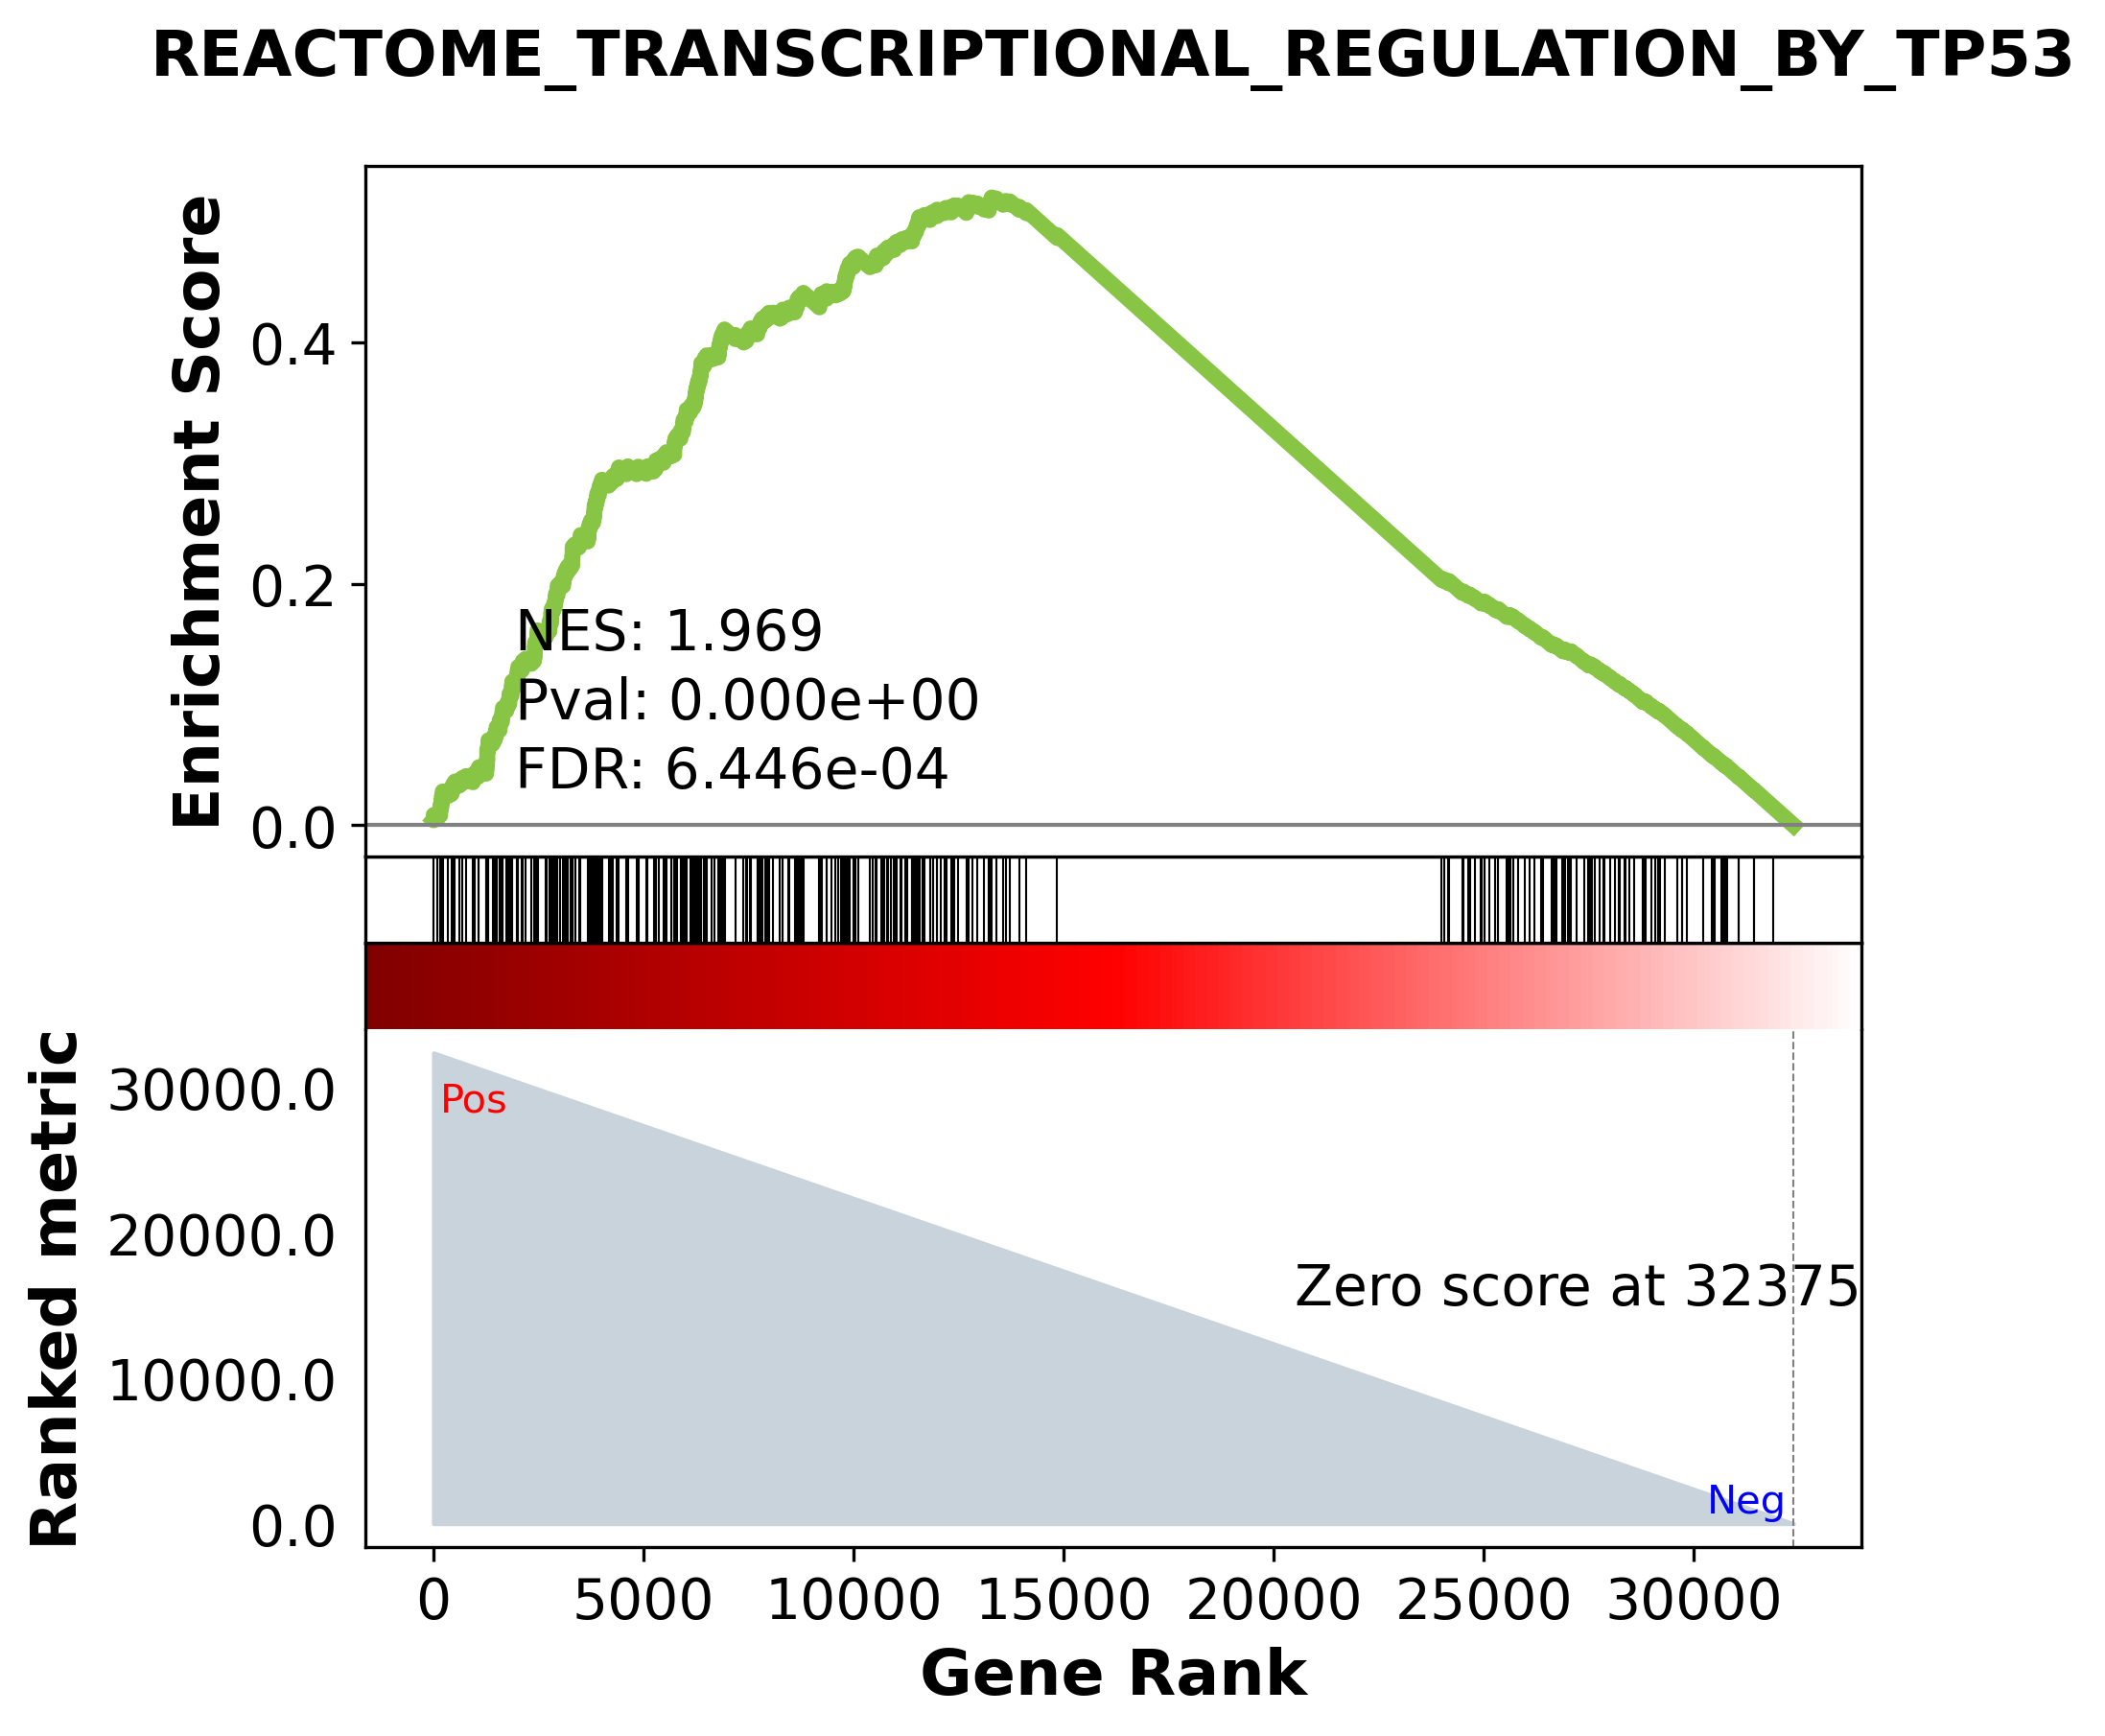
\includegraphics[width=0.7\textwidth,height=0.7\textheight,keepaspectratio]{Sections/Network_I/Resources/selective_pruning/gsea/REACTOME_TRANSCRIPTIONAL_REGULATION_BY_TP53.png}
  \caption{GSEA plot for the p53 pathway found in the smaller basal group. While there is a strong enrichment of this pathway is not unique to this group.}
\label{fig:N_I:gsea_p53_smallBasal}
\end{figure}

% Small basal commenting
The first part of the table \cref{tab:N_I:gsea_basal_reactome} contains the pathways found for the small basal group which are most involved in the cell functioning. It is striking that in most of the pathways found the lead genes are matched by the 5000 genes closest to the referential point. This denotes that from the 5000 genes there are many which play an important role in multiple pathways. Disruption to the cell cycle may also explain the poor survival prognosis. As seen in the GSEA plot from \cref{fig:ap:gsea_smallBasal}, the enrichment score is high but not many genes are hit in the high ranked genes (i.e. top 5000) and the most hit pathways is "NFE2L2 regulating anti oxidant detoxification enzymes". In the previous analysis done in this section suggested that \textit{TP53} is a marker for the smaller group. There is a 
strong signal of the \textit{p53} pathway as seen in \cref{fig:N_I:gsea_p53_smallBasal} but it is not unique to the smaller group.

% large basal commenting
In the second part of the \cref{tab:N_I:gsea_basal_reactome}, the pathways for the larger basal group are presented, which are mostly related to the immune response of the tissue. Especially the high match of the interferon pathways, which is expected as this groups contains the subtypes which were classified in the previous section \cref{s:clustering_analysis} as Medium IFNG and High IFNG. There was no unique signature found for Mes-like subgroup as the subtype shares pathways with the basal groups (interferon alpha, gamma pathways) as seen in the GSEA outputs from appendix \cref{fig:ap:gsea_largeBasal,fig:ap:gsea_mesLike}.

The table \cref{tab:N_I:gsea_luminal_reactome} contains the pathways found for the larger and infiltrated luminal subtypes. The pathway for latter mostly contains immunoglobulin related genes (e.g. \textit{IGV1-17}) denoting the infiltration of the immune cells in the bladder cancer samples. The pathways found for the large luminal are general and the lead genes have a low match ratio with the most 5000 most representative genes. This suggests that there is a less of a clear signal for a pathway to be enriched which might be explained by the size of the luminal group. 

% GSEA luminal table (reactome)
\begin{table}[!t]
  \centering
  \scriptsize
  \begin{tabularx}{\textwidth}{>{\hsize=1.7\hsize}X|>{\hsize=0.4\hsize}X|>{\hsize=0.4\hsize}X|>{\hsize=0.6\hsize}X|>{\hsize=0.4\hsize}X|>{\hsize=0.15\hsize}X}
    \toprule
    \textbf{Term} & \textbf{NES} & \textbf{FDR q-val} & \textbf{\# lead} & \textbf{\# matched} & \textbf{ratio} \\
    \midrule
    \multicolumn{6}{c}{\textbf{lumInf}} \\
    \midrule
    SCAVENGING OF HEME FROM PLASMA & 2.396 & 0 & 54 & 47 & 0.87 \\
    \midrule
    \multicolumn{6}{c}{\textbf{largeLuminal}} \\
    \midrule
    PARACETAMOL ADME & 2.016 & 0.003 & 15 & 15 & 1 \\
    \midrule
    EUKARYOTIC TRANSLATION ELONGATION & 1.864 & 0.029 & 73 & 5 & 0.068 \\
    \midrule
    SELENOAMINO ACID METABOLISM & 1.86 & 0.02 & 80 & 4 & 0.05 \\
    \midrule
    NONSENSE MEDIATED DECAY NMD & 1.832 & 0.025 & 81 & 8 & 0.099 \\
    \midrule
    SRP DEPENDENT COTRANSLATIONAL PROTEIN TARGETING TO MEMBRANE & 1.828 & 0.022 & 80 & 6 & 0.075 \\
    \midrule
    FORMATION OF WDR5 CONTAINING HISTONE MODIFYING COMPLEXES & 1.827 & 0.018 & 25 & 7 & 0.28 \\
    \midrule
    RESPONSE OF EIF2AK4 GCN2 TO AMINO ACID DEFICIENCY & 1.809 & 0.019 & 73 & 4 & 0.055 \\
    \midrule
    MITOCHONDRIAL FATTY ACID BETA OXIDATION & 1.789 & 0.023 & 28 & 18 & 0.643 \\
    \midrule
    BRANCHED CHAIN AMINO ACID CATABOLISM & 1.777 & 0.024 & 9 & 9 & 1 \\
    \midrule
    EUKARYOTIC TRANSLATION INITIATION & 1.77 & 0.025 & 76 & 5 & 0.066 \\
    \bottomrule
  \end{tabularx}
  \caption{Normalised Enrichment Score (NES), False Discovery Rate (FDR) q-val, and lead gene statistics for the large, infiltrated and mes-like group. The lead genes from a pathway are selected by GSEAPY based on when the NES reached its peak.}
  \label{tab:N_I:gsea_luminal_reactome}
\end{table}

GSEA was also applied to the hallmark gene set (50 pathways) and the oncogenic signature (189 gene sets), results that can be seen in Appendix \cref{ap:tab:gsea_hallmark,ap:tab:gsea_oncosig}. The GSEA outputs are harder to interpret especially the Onco Signature sets, but it can be observed that most of the unique pathways are found in both small basal and large luminal groups. Considering that the small basal group is considerably smaller than the large luminal, it suggests that the subtype should be study more.


% What are these 10 top genes
Returning to the small group and the pi scatter plot from \cref{fig:N_I:pi_smallBasal_comp},
seven out of the ten genes closest to the referential point were found to have biological significance in bladder cancer biology: \textit{GPX2, KRT13, ALDH3A1, KRT15, KRT4, AKR1B10, SOX2, TP63, RAPGEFL1, CAPNS2}. \textit{GPX2} is involved in squamous differentiation \citet{Naiki2018-fp}. Higher expression of \textit{KRT13} is associated with better response to chemotherapy and immunotherapy \citet{Yu2023-db}. The methylation of \textit{ALDH3A1}, along with \textit{HOXA9} and \textit{ISL1}, has been studied in non-muscle invasive bladder cancer and found to be a predictor of disease recurrence \citet{McLean2023-qk}. Additionally, higher expression of \textit{ALDH3A1} in bladder cancer is associated with higher tumour grade and has been studied in cancer stem cells \citet{Kim2013-th}. \textit{KRT4} is a basal keratin marker \citet{Marzouka2018-ge}. Both \textit{AKR1B10} and \textit{SOX2} are associated with cell and cancer aggressiveness \citet{Huang2021-bn, Chiu2020-xh}, while \textit{TP63} is a known squamous marker \citet{Robertson2017-mg}. This evidence supports the poor survival prognosis of the smaller group and indicates that this group warrants further study.


\subsection{Summary}

% Recapitulate the aims and what have been done
This subsection began with two aims: identifying the appropriate community detection method and exploring the integration of Transcription Factors (TF) into the network. The comparison at the start of the section (\ref{}) demonstrated that, despite the high computational cost of Stochastic Block Models (SBM), they offer more advantages over Modularity Maximisation algorithms such as Leiden. From a network perspective, the selective edge pruning method for integrating TFs was effective, as these nodes exhibited a higher degree. Thus, the two aims of the section were achieved.

% Significance in cancer
Throughout the selective edge experiments, it was remarkable to find that by using controls and prioritising non-TFs, a subset of 'naturally' well-connected TFs in the tumour dataset could be derived. The analysis in this section indicates that the subset of 98 TFs has important biological significance. Hierarchical clustering was applied to this subset of genes, yielding subtypes with significantly different survival outcomes (\cref{fig:N_I:sel_tfs_cs_analysis}). Group 5, or the small basal group of 20 patients, had the worst survival prognosis, with a less than 20\% chance of survival after 1.7 years (20 months). This group exhibited squamous markers, had a low immune response, and 7 out of the 10 most significantly expressed genes were studied in cancer. Some of these 7 genes are responsible for the aggressiveness of the tumours, while others can be targeted to improve treatment response.

% the two lists of basal/luminal
Using the analysis performed on the non-tumour dataset and the gene expression data from TCGA, the 98 TF genes were reduced to two different lists of markers for basal and luminal subtypes (\cref{tab:N_I:genes_lum_basal}). Many genes from these two lists were validated by other research work, which only confirmed and strengthened our findings.

% the list for non-tumour data
Extending the findings beyond cancer, some of the 98 TF genes were classified by their expression in the non-tumour dataset. The analysis performed (\cref{s:N:sel_tf_diff_status}) proposes three lists of genes specific to P0, UD, and AbsCa, as well as another three between these categories. This refined list of genes may help biologists better understand urothelium differentiation, which in turn will also aid in elucidating the basal/luminal molecular differences.

While the subset of TFs was informative for the Basal subgroup, it was less successful for the luminal subgroup. The previously derived luminal subtypes (consensus, TCGA, Lund, and the work in the previous chapter) are grouped into one large group. Looking at a known luminal marker, \textit{FGFR3}, it was observed that this gene has a low degree in the network. In addition, some other known markers were left out in the gene selection process (e.g., \textit{PPARG}). This may also be explained by the fact that luminal tumours are molecularly closer to differentiated bladder tissue, compared to the basal subtypes which are undifferentiated urothelium. The high variance introduced by the basal subtype might explain why other known gene markers were missed.

% Limitations
One of the limitations of the work done in selective edge pruning was that only ten control networks were used for comparison. This was due to the high computational time (a few hours) required to run the SBM, the lengthy process of loading the network output\footnote{During the network runs and SBM, a lot of metadata was saved, which helped to debug, understand, and analyse the networks. This made the network output fairly large, taking a considerable footprint of the RAM. For example, analysing the results for the 10 controls and experiments takes approximately 40GB of RAM.} and the limited time in a PhD project. Another possible limitation is using only 5000 genes for a network using SBM. As it will be seen in the next section \ref{}, the stochastic model is capable of finding smaller communities in a large network. This means that more genes can be included, but this will make the network very dense, so extra rules for edge pruning might be needed. However, from a biological perspective, re-running the selective edge pruning on larger networks and more controls may further enforce that there is a subset of TFs that are co-expressed with many genes in bladder cancer.

% Further work
Considering the limitations, the analysis performed suggests that both the subset of 98 TFs and the subtypes need more in-depth exploration, even selecting a few targeted genes to study the bladder response \textit{in-vitro}. It also suggests that the selective edge pruning is working and exhibits highly relevant biological results.
